%for a more compact document, add the option openany to avoid
%starting all chapters on odd numbered pages
%--------------------------------------------------------------------------
\documentclass[12pt]{cmuthesis}
%--------------------------------------------------------------------------
% This is a template for a CMU thesis.  It is 18 pages without any content :-)
% The source for this is pulled from a variety of sources and people.
% Here's a partial list of people who may or may have not contributed:
%
%        bnoble   = Brian Noble
%        caruana  = Rich Caruana
%        colohan  = Chris Colohan
%        jab      = Justin Boyan
%        josullvn = Joseph O'Sullivan
%        jrs      = Jonathan Shewchuk
%        kosak    = Corey Kosak
%        mjz      = Matt Zekauskas (mattz@cs)
%        pdinda   = Peter Dinda
%        pfr      = Patrick Riley
%        dkoes = David Koes (me)

% My main contribution is putting everything into a single class files and small
% template since I prefer this to some complicated sprawling directory tree with
% makefiles.

%--------------------------------------------------------------------------
% some useful packages
%--------------------------------------------------------------------------
\usepackage{times}
\usepackage{fullpage}
\usepackage{graphicx}
\usepackage{amsmath}
\usepackage[numbers,sort]{natbib}
\usepackage[backref,pageanchor=true,plainpages=false, pdfpagelabels, 
bookmarks,bookmarksnumbered,
%pdfborder=0 0 0,  %removes outlines around hyper links in online display
]{hyperref}
\usepackage{subfigure}
\usepackage{comment}   % package for block comment
\usepackage{graphicx}
\usepackage{hyperref}
\usepackage{url}
\usepackage{breakurl}
\usepackage{color}
\usepackage{xcolor}
\usepackage{listings}

% Approximately 1" margins, more space on binding side
%\usepackage[letterpaper,twoside,vscale=.8,hscale=.75,nomarginpar]{geometry}
%for general printing (not binding)

%--------------------------------------------------------------------------
\usepackage[letterpaper,twoside,vscale=.8,hscale=.75,nomarginpar,
hmarginratio=1:1]{geometry}
%--------------------------------------------------------------------------


\newcommand{\two}{\mspace{-2.0mu}}
\newcommand{\four}{\mspace{-4.0mu}}
\newcommand{\plus}{\mspace{-4.5mu}+\mspace{-3.5mu}}
\newcommand{\minus}{\mspace{-4.5mu}-\mspace{-3.5mu}}
\newcommand{\pp}{'\mspace{-2.0mu}'}

\newcommand{\xlb}[4]{#1\ifthenelse{\equal{#2}{0}}{}{_{\alpha #2}}
\mspace{-2.0mu}\genfrac{(}{)}{0pt}{1}
{\ifthenelse{\equal{#3}{0}}{0}{l #3}}
{\ifthenelse{\equal{#4}{0}}{0}{b #4}}}
%--------------------------------------------------------------------------
\newcommand{\xkv}[4]{#1\mspace{-5.0mu}\left(\mspace{-8.0mu}
\begin{smallmatrix}#2\four{}\four{}\mspace{-8.0mu}&
\pmb{\kappa}#3\\&\nu #4
\end{smallmatrix}\mspace{-5.0mu}\right)}

\newcommand{\evect}[6]{#1\mspace{-4.0mu}\left(\mspace{-8.0mu}
\begin{smallmatrix}#2\mspace{-8.0mu}&
\pmb{\kappa} #3 &b #5\\&\nu #4 &\alpha #6
\end{smallmatrix}\mspace{-5.0mu}\right)}

\newcommand{\varmat}[8]{\mspace{-5.0mu}\left(\mspace{-8.0mu}
\begin{smallmatrix}\ifthenelse{\equal{#3}{0}}
{\mspace{-8.0mu}&b_{#1}&b_{#2}\\&\alpha_{#1}&\alpha_{#2}}
{\ifthenelse{\equal{#7}{0}}{#1\mspace{-8.0mu}&\pmb{\kappa}#2#3
\mspace{-8.0mu}&\pmb{\kappa}#4#5\mspace{-8.0mu}&
\pmb{\kappa}#6\\&\nu#2&\nu#4&\nu#6} 
{#1\mspace{-8.0mu}&\pmb{\kappa}#2#3\mspace{-8.0mu}&\pmb{\kappa}#4#5
\mspace{-8.0mu}&\pmb{\kappa}#6#7\mspace{-8.0mu}&
\pmb{\kappa}#8\\&\nu#2&\nu#4&\nu#6&\nu#8}}
\end{smallmatrix}\mspace{-5.0mu}\right)}
%--------------------------------------------------------------------------
\newcommand{\EXP}[1]{\exp\mspace{-5.0mu}\left[#1\right]\mspace{-3.0mu}}

\newcommand{\tpp}[2]{\left(\mspace{-2.0mu}\xkv{\omega}{}{}{}#1
\xkv{\omega}{}{'}{'}#2\xkv{\omega}{}{\pp}{\pp}\mspace{-2.0mu}\right)}

\newcommand{\be} {\begin{eqnarray}}
\newcommand{\ee} {\end{eqnarray}}
\newcommand{\f}[2]{\ensuremath{\frac{\displaystyle{#1}}
{\displaystyle{#2}}}}
\newcommand{\lr}[1]{\langle{#1}\rangle}

\newcommand{\SUM}[2]{\ifthenelse{\equal{#1}{0}}
{\sum_{\alpha_{#2},b_{#2},l_{#2}}^{3,n,N}} 
{\ifthenelse{\equal{#1}{1}}{\sum_{\alpha_{#2},b_{#2}}^{3,n}}
{\sum_{\pmb{\kappa}#2,\nu#2}^{N,3n}}}}

\newcommand{\SUMprime}[2]{\ifthenelse{\equal{#1}{0}}
{\sum_{\alpha_{#2},b_{#2},l_{#2}}^{3,n,N}} 
{\ifthenelse{\equal{#1}{1}}{\sum_{\alpha_{#2},b_{#2}}^{3,n}}
{\sum_{\pmb{\kappa}^{'}#2,\nu#2}^{N,3n}}}}
%--------------------------------------------------------------------------
\newcommand{\SUMalpha}[2]{\ifthenelse{\equal{#1}{0}}
{\sum_{\alpha_{#2}}^{3}} 
{\ifthenelse{\equal{#1}{1}}{\sum_{\alpha_{#2},b_{#2}}^{3,n}}
{\sum_{\pmb{\kappa}#2,\nu#2}^{N,3n}}}}

\newcommand{\SUMalphap}[2]{\ifthenelse{\equal{#1}{0}}
{\sum_{\alpha'_{#2}}^{3}} 
{\ifthenelse{\equal{#1}{1}}{\sum_{\alpha'_{#2},b'_{#2}}^{3,n}}
{\sum_{\pmb{\kappa}#2,\nu#2}^{N,3n}}}}

\newcommand{\SUMb}[2]{\ifthenelse{\equal{#1}{0}}{\sum_{b_{#2}}^{n}} 
{\ifthenelse{\equal{#1}{1}}{\sum_{\alpha_{#2},b_{#2}}^{3,n}}
{\sum_{\pmb{\kappa}#2,\nu#2}^{N,3n}}}}

\newcommand{\SUMbp}[2]{\ifthenelse{\equal{#1}{0}}{\sum_{b'_{#2}}^{n}} 
{\ifthenelse{\equal{#1}{1}}{\sum_{\alpha'_{#2},b'_{#2}}^{3,n}}
{\sum_{\pmb{\kappa}#2,\nu#2}^{N,3n}}}}

\newcommand{\SUMl}[2]{\ifthenelse{\equal{#1}{0}}{\sum_{l_{#2}}^{N}} 
{\ifthenelse{\equal{#1}{1}}{\sum_{\alpha_{#2},b_{#2}}^{3,n}}
{\sum_{\pmb{\kappa}#2,\nu#2}^{N,3n}}}}

\newcommand{\SUMlp}[2]{\ifthenelse{\equal{#1}{0}}{\sum_{l'_{#2}}^{N}} 
{\ifthenelse{\equal{#1}{1}}{\sum_{\alpha'_{#2},b'_{#2}}^{3,n}}
{\sum_{\pmb{\kappa}#2,\nu#2}^{N,3n}}}}
%--------------------------------------------------------------------------
\newcommand{\abcdt}[5]{\mspace{-4.0mu}\left(\mspace{-8.0mu}
\begin{smallmatrix}&\ifthenelse{\equal{#1}{}}{a}{#1}&
\ifthenelse{\equal{#3}{}}{c}{#3}\\&
\ifthenelse{\equal{#2}{}}{b}{#2}&\ifthenelse{\equal{#4}{}}{d}{#4}
\end{smallmatrix}\mspace{-2.0mu};
\ifthenelse{\equal{#5}{}}{t}{#5}\right)}

\newcommand{\abcd}[4]{\mspace{-4.0mu}\left(\mspace{-8.0mu}
\begin{smallmatrix}&\ifthenelse{\equal{#1}{}}{a}{#1}&
\ifthenelse{\equal{#3}{}}{c}{#3}\\&
\ifthenelse{\equal{#2}{}}{b}{#2}&\ifthenelse{\equal{#4}{}}{d}{#4}
\end{smallmatrix}\mspace{-3.0mu}\right)}

\newcommand{\abt}[3]{\mspace{-4.0mu}\left(\mspace{-8.0mu}
\begin{smallmatrix}&\ifthenelse{\equal{#1}{}}{a}{#1} \\&
\ifthenelse{\equal{#2}{}}{b}{#2}
\end{smallmatrix}\mspace{-2.0mu};
\ifthenelse{\equal{#3}{}}{t}{#3}\right)}

\newcommand{\ab}[2]{\mspace{-4.0mu}\left(\mspace{-8.0mu}
\begin{smallmatrix}&\ifthenelse{\equal{#1}{}}{a}{#1} \\&
\ifthenelse{\equal{#2}{}}{b}{#2}
\end{smallmatrix}\mspace{-3.0mu}\right)}

\newcommand{\kvbat}{\mspace{-4.0mu}\left(\mspace{-8.0mu}
\begin{smallmatrix} &\pmb{\kappa} &b \\ &\nu &\alpha
\end{smallmatrix}\mspace{-2.0mu};t\right)}

\newcommand{\kvbatp}{\mspace{-4.0mu}\left(\mspace{-8.0mu}
\begin{smallmatrix} &\pmb{\kappa} &b' \\ &\nu &\alpha'
\end{smallmatrix}\mspace{-2.0mu};t\right)}
%--------------------------------------------------------------------------
\newcommand{\kvbaw}{\mspace{-4.0mu}\left(\mspace{-8.0mu}
\begin{smallmatrix} &\pmb{\kappa} &b \\ &\nu &\alpha
\end{smallmatrix}\mspace{-2.0mu};\omega\right)}

\newcommand{\kvbawp}{\mspace{-4.0mu}\left(\mspace{-8.0mu}
\begin{smallmatrix} &\pmb{\kappa} &b' \\ &\nu &\alpha'
\end{smallmatrix}\mspace{-2.0mu};\omega\right)}

\newcommand{\kvba}{\mspace{-4.0mu}\left(\mspace{-8.0mu}
\begin{smallmatrix} &\pmb{\kappa} &b \\ &\nu &\alpha
\end{smallmatrix}\mspace{-3.0mu}\right)}

\newcommand{\kvbap}{\mspace{-4.0mu}\left(\mspace{-8.0mu}
\begin{smallmatrix} &\pmb{\kappa} &b' \\ &\nu &\alpha'
\end{smallmatrix}\mspace{-3.0mu}\right)}

\newcommand{\kpvba}{\mspace{-4.0mu}\left(\mspace{-8.0mu}
\begin{smallmatrix} &\pmb{\kappa}^{'} &b \\ &\nu &\alpha
\end{smallmatrix}\mspace{-3.0mu}\right)}

\newcommand{\kva}{\mspace{-4.0mu}\left(\mspace{-8.0mu}
\begin{smallmatrix} &\pmb{\kappa} \\ &\nu &\alpha
\end{smallmatrix}\mspace{-3.0mu}\right)}

\newcommand{\kvap}{\mspace{-4.0mu}\left(\mspace{-8.0mu}
\begin{smallmatrix} &\pmb{\kappa} \\ &\nu &\alpha'
\end{smallmatrix}\mspace{-3.0mu}\right)}
%--------------------------------------------------------------------------
\newcommand{\kvb}{\mspace{-4.0mu}\left(\mspace{-8.0mu}
\begin{smallmatrix} &\pmb{\kappa} &b \\ &\nu 
\end{smallmatrix}\mspace{-3.0mu}\right)}

\newcommand{\kvbp}{\mspace{-4.0mu}\left(\mspace{-8.0mu}
\begin{smallmatrix} &\pmb{\kappa} &b' \\ &\nu 
\end{smallmatrix}\mspace{-3.0mu}\right)}

\newcommand{\kvt}{\mspace{-4.0mu}\left(\mspace{-8.0mu}
\begin{smallmatrix}&\pmb{\kappa} \\&\nu
\end{smallmatrix}\mspace{-2.0mu};t\right)}

\newcommand{\kpvt}{\mspace{-4.0mu}\left(\mspace{-8.0mu}
\begin{smallmatrix}&\pmb{\kappa}^{'} \\&\nu
\end{smallmatrix}\mspace{-2.0mu};t\right)}

\newcommand{\kvw}{\mspace{-4.0mu}\left(\mspace{-8.0mu}
\begin{smallmatrix}&\pmb{\kappa} \\&\nu
\end{smallmatrix}\mspace{-2.0mu};\omega\right)}

\newcommand{\kv}{\mspace{-4.0mu}\left(\mspace{-8.0mu}
\begin{smallmatrix}&\pmb{\kappa} \\&\nu
\end{smallmatrix}\mspace{-3.0mu}\right)}
%--------------------------------------------------------------------------
\newcommand{\lbt}{\mspace{-4.0mu}\left(\mspace{-8.0mu}
\begin{smallmatrix}&l \\&b\end{smallmatrix}\mspace{-2.0mu};t\right)}

\newcommand{\lbtp}{\mspace{-4.0mu}\left(\mspace{-8.0mu}
\begin{smallmatrix}&l' \\&b'\end{smallmatrix}\mspace{-2.0mu};t\right)}

\newcommand{\lt}{\mspace{-4.0mu}\left(\mspace{-8.0mu}
\begin{smallmatrix}&l\end{smallmatrix}\mspace{-2.0mu};t\right)}

\newcommand{\ltp}{\mspace{-4.0mu}\left(\mspace{-8.0mu}
\begin{smallmatrix}&l'\end{smallmatrix}\mspace{-2.0mu};t\right)}

\newcommand{\lb}{\mspace{-4.0mu}\left(\mspace{-8.0mu}
\begin{smallmatrix}&l \\&b\end{smallmatrix}\mspace{-3.0mu}\right)}

\newcommand{\lbp}{\mspace{-4.0mu}\left(\mspace{-8.0mu}
\begin{smallmatrix}&l' \\&b'\end{smallmatrix}\mspace{-3.0mu}\right)}
%--------------------------------------------------------------------------

% Provides a draft mark at the top of the document. 
\draftstamp{\today}{DRAFT}

\begin {document} 
\frontmatter

A) Signature Page – see Section 4
s
%initialize page style, so contents come out right (see bot) -mjz
\pagestyle{empty}

B) Title Page – see Section 4
\title{ %% {\it \huge Thesis Proposal}\\
{\bf Thermal Modeling of Disordered Materials}}
\author{Jason M. Larkin}
\date{August 2013}
\Year{2013}
\trnumber{}



\committee{
\href{http://www.cmu.edu/me/people/alan-j-h-mcgaughey.html}
{Alan J. H. McGaughey, Chair} \\
\href{http://www.cmu.edu/me/people/jonathan-a-malen.html}
{Jonathan Malen} \\
\href{http://www.ce.cmu.edu/people/faculty/maloney.html}
{Craig Maloney} \\
\href{http://www.cmu.edu/physics/people/faculty/widom.html}
{Michael Widom}
}

\support{}
\disclaimer{}

6.2 Preliminaries



C) Copyright Notice – should follow the title page, on a separate page, if statutory copyright in the dissertation has been or is to be claimed

%--------------------------------------------------------------------------
% copyright notice generated automatically from Year and author.
% permission added if \permission{} given.

\keywords{Phonon}

\maketitle

\begin{dedication}
For my dog
\end{dedication}

\pagestyle{plain} % for toc, was empty

%% Obviously, it's probably a good idea to break the various sections of your thesis
%% into different files and input them into this file...

\begin{abstract}
A short summary.
\end{abstract}

\begin{acknowledgments}
test
\end{acknowledgments}

D) Acknowledgments – must include financial support acknowledgment as discussed in Section 5

E) Abstract – should not exceed 350 words; see Section 2

F) Table of Contents – with page references

G) List of Tables – with titles and page references

H) List of Figures and Illustrations – with titles and page references.



\tableofcontents
\listoffigures
\listoftables
%--------------------------------------------------------------------------
\mainmatter

%% Double space document for easy review:
%\renewcommand{\baselinestretch}{1.66}\normalsize

% The other requirements Catherine has:
%
%  - avoid large margins.  She wants the thesis to use fewer pages, 
%    especially if it requires colour printing.
%
%  - The thesis should be formatted for double-sided printing.  This
%    means that all chapters, acknowledgements, table of contents, etc.
%    should start on odd numbered (right facing) pages.
%
%  - You need to use the department standard tech report title page.  I
%    have tried to ensure that the title page here conforms to this
%    standard.
%
%  - Use a nice serif font, such as Times Roman.  Sans serif looks bad.
%
% Other than that, just make it look good...

%--------------------------------------------------------------------------

I get the requirements here
\href{http://www.cit.cmu.edu/current_students/graduates/thesis_dissertation_policies.html}{http://www.cit.cmu.edu/current_students/graduates/thesis_dissertation_policies.html}

6. PREPARATION OF THE MANUSCRIPT: FORM

 

6.1 Title – Your thesis or dissertation will be a valuable source for other scholars only if it can be located easily. Modern retrieval systems use the words in the title—and sometimes a few other descriptive words—to locate your document. It is essential that the title be a meaningful description of the content of your dissertation. Avoid highly specialized terms to the extent possible, and use word substitutes for formulas, symbols, superscripts, Greek letters, etc.

 



 

6.3 Body of thesis or dissertation

A) Introduction

B) Main Body – with larger divisions and more important minor divisions indicated by suitable, consistent headings

C) Summary and Conclusions – highlighting the key findings and conclusions of the work presented. For engineering and science theses and dissertations, this section often also includes recommendations for follow-up research.

D) References – >see discussion in Section 6.9

E) Appendices – each appendix should have a title and be listed in the Table of Contents

 

6.4 Page Numbering

Each page in a thesis or dissertation should be assigned a number. The following plan of page numbering generally is accepted:

A) For Preliminaries – use small Roman numerals (i, ii, iii, iv, etc.). The numbering begins with ii; the title page counts as page i, but the number does not appear.

B) For Remainder of Thesis or Dissertation – including the text, illustrations, appendices, and bibliography, use Arabic numerals (1, 2, 3, 4, etc.). Each page must be numbered. Try to avoid use of letter suffixes such as 10a, 10b. The numbering begins with 1 and runs consecutively to the end of the dissertation.

C) For More Than One Volume – each volume should contain a title page duplicating the title page of the first volume. If the volumes are separate entities, identify them further as Volume I, II, etc. In any case, the numbering may follow consecutively from one volume to another, or begin with Arabic 1 at each new title page.

 

6.5 Footnotes

If footnotes are needed, they should be placed at the bottom of the page below a 1.5 inch underscore (starting at the left border). The first line of each footnote should be indented 0.5 inches and identified by a raised numeral corresponding to that used in the test. Footnotes should be numbered consecutively throughout each chapter.




\chapter{\label{chapter:vc}Predicting alloy vibrational mode properties 
using lattice dynamics calculations, molecular dynamics simulations, 
and the virtualcrystal approximation}

%--------------------------------------------------------------------------
%\begin{abstract}
%--------------------------------------------------------------------------
The virtual crystal (VC) approximation for mass disorder is evaluated by
examining two model alloy systems: Lennard-Jones argon and Stillinger-Weber
silicon. 
In both material systems, the perfect crystal is alloyed with a heavier mass
species up to equal concentration.
The analysis is performed using molecular dynamics simulations and lattice
dynamics calculations.
Mode frequencies and lifetimes are first calculated by treating the disorder
explicitly and under the VC approximation, with differences found in the
high-concentration alloys at high frequencies. 
Notably, the lifetimes of high-frequency modes are underpredicted using the
VC approximation, a result we attribute to the neglect of higher-order terms 
in the model used to include point-defect scattering.
The mode properties are then used to predict thermal conductivity under the
VC approximation.
For the Lennard-Jones alloys, where high-frequency modes make a significant
contribution to thermal conductivity, the high-frequency lifetime
underprediction leads to an underprediction of thermal conductivity compared
to predictions from the Green-Kubo method, where no assumptions about the
thermal transport are required.
Based on observations of a minimum mode diffusivity, we propose a correction
that brings the VC approximation thermal conductivities into better 
agreement with the Green-Kubo values. 
For the Stillinger-Weber alloys, where the thermal conductivity is dominated
by low-frequency modes, the high-frequency lifetime underprediction does not
affect the thermal conductivity prediction and reasonable agreement is found
with the Green-Kubo values. 
%--------------------------------------------------------------------------
%\end{abstract}
%--------------------------------------------------------------------------

%--------------------------------------------------------------------------
\section{\label{S:Introduction}Introduction}
%--------------------------------------------------------------------------

Due to their potentially low thermal conductivities, 
disordered materials (e.g., alloys, amorphous solids, aerogels) 
are used in 
applications ranging from thermoelectric energy conversion to 
thermally insulating barriers.
\cite{graebner_phonon_1986,cahill_lattice_1988,lu_thermal_1992,
chen_recent_2003,clarke_thermal_2005,snyder_complex_2008,
minnich_bulk_2009,toberer_phonon_2011,zebarjadi_perspectives_2012,
schiffres_gas_2012} 
Disordered lattices are a subgroup of disordered materials where 
the atomic positions follow a lattice structure but the 
constituent species are spatially random. Examples include isotopic 
solids, where the species have the same electronic structure but 
small mass variations,\cite{tamura_isotope_1983,lindsay_thermal_2012} 
and alloys, our focus here, where at least two distinct 
species are present.\cite{abeles_thermal_1962,abeles_lattice_1963}

We further restrict our focus to dielectric or semiconducting solids,  
where the heat is conducted by the atomic vibrational modes. 
Predicting the thermal conductivity of such materials 
requires the properties of the full spectrum of vibrational modes.
\cite{ziman_electrons_2001,feldman_thermal_1993,allen_diffusons_1999} 
Accurate predictions of these properties for 
crystalline systems (i.e., perfect lattices)  
can be made with anharmonic lattice dynamics (ALD) theory 
using input from density functional theory (DFT)  
calculations.\cite{broido_intrinsic_2007,ward_intrinsic_2010,
lindsay_thermal_2012,garg_role_2011,shiga_microscopic_2012,
tian_phonon_2012,shiomi_thermal_2011,esfarjani_heat_2011,
li_thermal_2012,luckyanova_coherent_2012}
Computational costs limit DFT calculations to less than 100 atoms, 
however, making it challenging to explicitly incorporate the effects 
of disorder.
\cite{ward_ab_2009,garg_role_2011,bao_first-principles_2012,
sosso_thermal_2012,lindsay_thermal_2012,tian_phonon_2012,
li_thermal_2012}

Disorder is typically included in the ALD framework using Abeles' 
virtual crystal (VC) approximation, whereby the disordered  
solid is replaced with a perfect VC with properties 
equivalent to an averaging over the disorder 
(e.g., atomic mass, bond strength).\cite{abeles_lattice_1963}
The ALD calculations are performed on a small 
unit cell with the averaged properties 
(i.e., all vibrational modes are phonons) and 
phonon-phonon and phonon-disorder scattering 
are included as perturbations.
\cite{abeles_lattice_1963,tamura_isotope_1983,garg_role_2011,
tian_phonon_2012,lindsay_thermal_2012} 
Except for low-frequency (long-wavelength) acoustic modes,
the general validity of this assumption is unclear. 
We will refer to this approach as VC-ALD. 
Recent work using DFT calculations and the VC-ALD approach has 
modeled disordered lattices with relatively large 
($\sim$ 10-100 W/m-K)
\cite{garg_role_2011,lindsay_thermal_2012,li_thermal_2012} and 
small ($\sim$ 1 W/m-K)\cite{tian_phonon_2012} 
thermal conductivities. No comprehensive study has 
been performed to assess the applicability of the VC-ALD approach for a 
range of disorder strength.

The objective of this study is to investigate the use of the VC 
approximation for predicting the vibrational mode properties and 
thermal conductivity of alloys by a detailed comparison 
of three predictive methods: (i) molecular dynamics (MD)-based 
normal mode decomposition (NMD), (ii) MD-based Green-Kubo (GK), 
and (iii) VC-ALD. By using computationally-inexpensive  
empirical potentials for argon [Lennard-Jones (LJ) at a temperature of 10 K]
\cite{ashcroft_solid_1976} 
and silicon [Stillinger-Weber (SW) at a temperature of 300 K],
\cite{stillinger_computer_1985}   
we can self-consistently study the effects of disorder both explicitly 
and as a perturbation. For both materials, the perfect lattice is 
disordered with a heavier mass species up to equal 
concentration, spanning 
a range of small to large disorder. By spanning this range, 
the limits of the perturbative models are examined.

The remainder of the paper is organized as follows. 
In Section \ref{S:Theoretical}, the theoretical 
formulation of thermal transport in ordered and disordered solids 
and the computational framework are described. 
In Section \ref{S:Vibrational}, the frequencies, 
group velocities, lifetimes, and diffusivities of the 
vibrational modes of the LJ argon alloys are 
predicted when the disorder is explicitly modeled and when it is 
treated as a perturbation in the VC approximation. 
A breakdown of the VC-ALD method is identified by a comparison 
with the VC-NMD method in 
Section \ref{S:From VC-ALD}   
and a correction is suggested in Section \ref{S:Diffusivities}. 
The vibrational 
mode properties are then used to predict thermal conductivities 
in Section \ref{S:Thermal Conductivity}, 
allowing for a comparison to the predictions of the top-down  
GK method, where no assumptions about the nature of the 
thermal transport are required. The vibrational mode properties and 
thermal conductivity of the SW silicon alloys, where low-frequency modes 
dominate the thermal conductivity, are predicted in 
Section \ref{S:SW} to provide a comparison and contrast to the 
LJ argon alloys. 

% NOT USED:
% There is a need to model the thermal conductivity of disordered lattices 
% with intrinsically high and low thermal conductivity. 

% Both of these alloys have relatively high thermal conductivities 
% (on the order of 1-10 W/m-K at 300 K). However, in the heavily disordered 
% system In(As,P) (mass ratio of 3.7) worse agreement with the Abeles theory 
% is observed.

% not used yet...
% Experimental measurements of isotopically pure and Ge-doped 
% Si epitaxial layers demonstrate the original theory by Abeles can predict 
% thermal conductivity in dilute alloys. Abeles also found good agreement 
% with dilute predictions for both experimental measurements of both 
% Si-Ge alloys and also (Ga,In)As alloys.\cite{abeles_lattice_1963} However, 
% both of these alloy systems have a relatively high thermal conductivities 
% (on the order of 1-10 W/m-K at 300 K). However, in the heavily disordered 
% system In(As,P) (mass ratio of 3.7) worse agreement with the Abeles theory 
% is observed. 

%--------------------------------------------------------------------------
\section{\label{S:Theoretical}Theoretical and Computational Framework}
%--------------------------------------------------------------------------

%--------------------------------------------------------------------------
\subsection{\label{S:Thermal Theory}
Thermal Conductivity Prediction}
%--------------------------------------------------------------------------

To predict the thermal conductivity of a disordered lattice, 
one begins with the theory for a perfect lattice. For a perfect lattice, 
all vibrational modes are phonon modes, which by 
definition are delocalized, propagating plane waves.
\cite{ziman_electrons_2001} Using the single-mode relaxation
time approximation \cite{ziman_electrons_2001} to solve 
the Boltzmann transport equation gives an 
expression for thermal conductivity in direction $\mathbf{n}$,
\begin{equation}\label{EQ:k_vib}
\begin{split}
k_{ph,\mathbf{n}}=&\sum_{\pmb{\kappa}} \sum_\nu c_{ph}\kv 
v^{2}_{g,\mathbf{n}}\kv \tau\kv.
\end{split}
\end{equation}
Here, the sum is over the phonon modes in the first Brillouin 
zone, $\pmb{\kappa}$ is the wave vector, and 
$\nu$ labels the polarization branch.  
The phonon mode has frequency $\omega\kv$, 
volumetric specific heat $c_{ph}\kv$, 
$\mathbf{n}$-component of the 
group velocity vector ${v}_{g,\mathbf{n}}\kv$, 
and lifetime $\tau\kv$. 

The relaxation time approximation has been found to be valid  
for lower thermal conductivity materials 
(e.g., Si and SiGe alloys),
\cite{broido_intrinsic_2007,ward_intrinsic_2010,garg_role_2011} 
while larger thermal conductivity 
materials such as GaN and diamond require an  
iterative solution to the BTE for more accurate predictions 
using Eq. \eqref{EQ:k_vib}.
\cite{ward_ab_2009,lindsay_thermal_2012} 
For the crystalline LJ argon and SW silicon phases, 
the lattices and the components of their 
thermal conductivity tensors are cubically symmetric, 
so that we will refer to 
$k_{ph}$ as an isotropic scalar thermal conductivity. 
This isotropy will hold for disordered lattices 
in the infinite-size limit. 
Since MD simulations are classical 
and obey Maxwell-Boltzmann 
statistics,\cite{mcquarrie_statistical_2000} the volumetric 
specific heat is $k_{\text{B}}/V$ per mode in the harmonic limit, where $V$ 
is the system volume and $k_{\text{B}}$ is the Boltmann constant. 
This harmonic approximation for specific heat has been shown to be valid 
for LJ argon and SW silicon at the temperatures of interest here
\cite{mcgaughey_quantitative_2004,goicochea_thermal_2010} 
and is used so that direct comparisons can be made between 
the MD- and lattice dynamics-based methods.

For disordered systems, the vibrational modes are no 
longer pure plane-waves (i.e., phonon modes), except in the low-frequency 
(long-wavelength) limit. When applied in the classical limit, 
the Allen-Feldman (AF) theory computes 
the contribution of diffusive, non-propagating modes (i.e., diffusons) 
to thermal conductivity from\cite{allen_thermal_1993} 
\begin{equation}\label{EQ:M:k_AF}
k_{AF} = \sum_{diffusons} \frac{k_{\text{B}}}{V} D_{AF,i}(\omega_i),
\end{equation}
where $D_{AF,i}$ is the mode diffusivity and $\omega_i$ is the 
frequency of the $i$th diffuson. The diffusivity of diffusons 
can be calculated from harmonic lattice dynamics theory.
\cite{allen_thermal_1993,feldman_thermal_1993,feldman_numerical_1999} 

Assuming that all vibrational modes travel with the sound speed, $v_s$, and 
scatter over a distance of the lattice constant, $a$, 
a high-scatter (HS) limit of thermal conductivity in the classical 
limit is\cite{cahill_lattice_1988} 
\begin{equation}\label{EQ:M:k_AF,HS}
k_{HS} = \frac{k_{\text{B}}}{V_b}b v_s a,
\end{equation}
where $V_b$ is the volume of the unit cell and $b$ is the number of atoms 
in the unit cell. The HS limit will be used to 
discuss the differences between the LJ argon and SW silicon alloys. 

% The relative contribution of both
% phonons and diffusons to the total vibrational 
% conductivity has been estimated 
% to be approximately equal for a-Si,\cite{he_heat_2011} while earlier 
% studies find that $k_{ph}$ is substatiantially less.
% \cite{feldman_numerical_1999} 

%--------------------------------------------------------------------------
\subsection{\label{S:Virtual Crystal}Virtual Crystal Approximation}
%--------------------------------------------------------------------------

Under the VC approximation, the disordered solid is replaced with 
a perfect, single-species crystal with properties (e.g., density, 
cohesive energy) equivalent to an averaging over the disorder 
(e.g., atomic mass, bond strength).\cite{abeles_lattice_1963}
The VC approximation is visualized for an alloy in Figs. 
\ref{F:supercells}(a) and \ref{F:supercells}(b), where 
a mass-disordered supercell is replaced by a perfect 
crystal with an averaged mass. 
Abeles first introduced the concept of a VC to predict the
thermal conductivity of SiGe, GaAs/InAs, and InAs/InP alloys.
\cite{abeles_lattice_1963} Klemens-Callaway theory, 
which is valid for low-frequency modes and small disorder, was used to 
model the phonon-phonon and phonon-defect scattering.
\cite{abeles_lattice_1963,klemens_scattering_1955,klemens_thermal_1957,
callaway_model_1959,mattis_phonon_1957,kamitakahara_vibrations_1974} 
The Abeles theory is conceptually simple, treating both
disorder and anharmonicity as perturbations, and leads to 
a closed-form analytical function for the thermal conductivity.
With the use of phenomenological  
fitting parameters, good agreement between the predictions and 
experimental measurements 
was found for SiGe and GaAs/InAs alloys. Deviations were observed 
for InAs/InP alloys at large concentrations of 
InP, which were attributed to the large mass ratio of 3.7 between 
indium and phosphorus.\cite{abeles_lattice_1963}

When considering alloys, it is important to note that 
the overall disorder strength is determined by the mass ratio, 
the stiffness ratio, and the alloy concentration.
Cahill and co-workers found that as little as 
$6.2\times10^{19}$ cm$^{-3}$ germanium reduces the thermal conductivity 
of epitaxial silicon layers by a factor of two.
\cite{cahill_thermal_2004}  
Using the Abeles theory, they explained this result 
by mass perturbative disorder alone (the Ge/Si mass ratio is 2.6).
\cite{cahill_thermal_2004,cahill_thermal_2005} 
The relative effects of bond and mass disorder were investigated 
computationally using MD simulations by Skye and 
Schelling for SiGe alloys up to equal concentration.
\cite{skye_thermal_2008} They also found that mass disorder is 
the dominant scattering mechanism. Subsequent studies have modeled the 
effect of differing species by only including 
atomic mass differences.\cite{landry_thermal_2009,tian_enhancing_2012}

Unlike the phenomenological 
Abeles theory, the VC-ALD approach predicts thermal conductivity 
by directly summing over the modes of the full vibrational spectrum, 
with phonon-phonon and phonon-defect scattering treated as 
perturbations.
\cite{garg_role_2011,tian_phonon_2012,lindsay_thermal_2012} 
In the VC-ALD method, the phonon-phonon scattering is  
predicted using ALD.\cite{turney_predicting_2009,esfarjani_heat_2011} 
The phonon-defect scattering is treated 
using perturbative methods that can handle mass and/or bond disorder.
\cite{klemens_scattering_1955,klemens_thermal_1957,mattis_phonon_1957,
tamura_isotope_1983} 
In Ni$_{0.55}$Pd$_{0.45}$, 
which has a large mass ratio (1.8) and concentration of each species, 
experimental measurements of   
vibrational frequencies and linewidths agree well with 
predictions from the perturbative mass-disorder theory.
\cite{mattis_phonon_1957,kamitakahara_vibrations_1974,tamura_isotope_1983} 

Using DFT methods to predict 
the mode-specific phonon properties of the VC, Lindsay and Broido 
found good agreement between VC-ALD and experimental measurements of 
thermal conductivity for 
isotopically defected GaN (the gallium isotopes have concentrations of 
0.6 and 0.4 and a mass ratio of 1.03).\cite{lindsay_thermal_2012} 
Garg et al. used DFT calculations with VC-ALD   
to predict the thermal conductivity of SiGe alloys 
for all concentrations at a temperature of 300 K, 
obtaining good agreement with experiment.\cite{garg_role_2011}  
By including disorder explicitly in their ALD calculations, the predicted 
thermal conductivity decreased by 15$\%$. 
Isotopically-defected GaN and low concentration SiGe alloys 
have relatively large 
thermal conductivities at a temperature of 300 K ($\sim$ 100 W/m-K). 
Li et al. used DFT calculations with VC-ALD to predict the thermal 
conductivity of Mg$_2$Si$_x$Sn$_{1-x}$ ($\sim$ 10 W/m-K) 
in good agreement with 
experimental measurements for all concentrations.\cite{li_thermal_2012}
The VC-ALD approach has also been used to predict the effect of interfacial 
mixing in GaAs/AlAs superlattices, but the thermal 
conductivity predictions were not compared with experimental 
measurements.\cite{luckyanova_coherent_2012}  
In our survey of experimental measurements and numerical modeling, 
we find that 
VC predictions tend to be accurate when the disordered lattice 
thermal conductivity 
is significantly above the high-scatter limit [Eq. \eqref{EQ:M:k_AF,HS}],  
which tends to be around 1 W/m-K.
\cite{abeles_lattice_1963,kamitakahara_vibrations_1974,
cahill_thermal_2004,cahill_thermal_2005,cahill_lattice_1988,
garg_role_2011,lindsay_thermal_2012} 

An ALD study using phonon properties from DFT calculations for 
crystalline PbTe\cite{shiga_microscopic_2012} predicted 
thermal conductivities of 2 W/m-K at a temperature of 300 K 
in fair agreement with experiment. 
For PbTeSe alloys, a VC-ALD 
study predicted a small thermal conductivity reduction compared to the 
perfect crystals.\cite{tian_phonon_2012} Experimental results are limited 
for these alloys,\cite{kudman_thermoelectric_1972,pei_convergence_2011} 
making it difficult to asses the validity of the VC-ALD approach for 
materials whose thermal conductivities approach the high-scatter limit.

Given all these results, it is unclear what limitations exist for 
using the VC approach. 
In this study, we will consider a low thermal conductivity alloy  
using the LJ potential and a high thermal conductivity alloy using the 
SW potential. The computational studies discussed above were 
limited to VC-ALD 
because of DFT calculation costs. Our use of computationally 
inexpensive empirical potentials allows us to include the disorder 
explicitly and as a perturbation and to compare the predictions. 

% NOT USED:
% Many experimental trends in thermal conductivity 
% of a range of materials 
% can be explained using the VC approximation.(cite) For example,
% the reduced thermal conductivity of Ge versus Si is partly explained 
% by both the increased mass and decreased bulk modulus (stiffness) of the 
% lattice,(cite) which has the effect of reducing the phonon group 
% velocities. The same effect can be seen in alloy systems.(cite)
% Sound speeds of alloys: CRC, (Cahill-Pohl).

%--------------------------------------------------------------------------
\begin{figure}
\begin{center}
\mbox{\subfigure{
(a)
\includegraphics[scale=0.13]
{/home/jason/disorder/si/si_conv_2x2x2_disorder-4.eps}
\subfigure{
(b)
\includegraphics[scale=0.13]
{/home/jason/disorder/si/si_conv_2x2x2_perfect-4.eps}}}}
\vspace*{0mm}
\end{center}
\caption{\label{F:supercells} 
(a) Explicitly disordered supercell of 
Si and ``heavy'' Si ([100] direction into the paper).
\cite{momma_vesta:_2008} 
(b) Equivalent VC supercell with one averaged mass. 
The sphere size represents increasing mass only, no bond disorder 
is considered. The 8-atom conventional cubic unit cell is shown 
in (b). 
}
\end{figure}
%--------------------------------------------------------------------------

%--------------------------------------------------------------------------
\begin{figure}
\begin{center}
\centering
\includegraphics[scale=0.2]
{/home/jason/disorder/paper/vc/fig1.eps}
\end{center}
\caption{\label{F:supercells} 
(a) Explicitly disordered alloy supercell of 
silicon and ``heavy'' silicon ([100] direction into the page).
\cite{momma_vesta:_2008} 
(b) Equivalent VC supercell with one averaged mass. 
The sphere size represents increasing mass only, no bond disorder 
is considered. The 8-atom conventional cubic unit cell is shown 
in (b). 
}
\end{figure}
%--------------------------------------------------------------------------


%--------------------------------------------------------------------------
\subsection{\label{S:Calculation}Calculation and Simulation Details}
%--------------------------------------------------------------------------

The key to explicitly incorporating the effects of disorder 
is to use large disordered supercells. 
Perfect and disordered lattice supercells are generated using the 
conventional unit cells for LJ argon ($n=4$) and 
SW silicon ($n=8$), where $n$ is the number of atoms 
in the unit cell. 
Supercells are built cubically with size $N_0$, where $N_0$ is the 
number of unit cell repetitions in the three  
spatial directions. Supercells up to $N_0 = 12$ 
(6,096 atoms) are used for the LJ argon calculations. For SW silicon, 
$N_0 = 8$ (4,096 atoms) is used for 
the MD-based NMD calculations and $N_0 \le 42$ (592,704 atoms) 
is used for the MD-based GK and VC-ALD.  

Disorder is created by randomly specifying the masses of the atoms 
on the lattice. 
The composition of each lattice is labeled by $m^i_{1-c}m^j_{c}$,  
where (i) $m^i=1$ and $m^j=3$ in 
LJ units for argon, and (ii) $m^i=m_{Si}$ and $m^j=2.6m_{Si}$ 
for SW silicon and ``heavy silicon'', which has the mass of germanium. 
Concentrations, $c$, of $0,0.05,0.15$ and $0.5$ are considered. 
% Based on the previous works of others, we only consider mass disorder.

For LJ argon, the lattice constant 
at a temperature of 10 K is 5.290 $\AA$.\cite{mcgaughey_phonon_2004} 
The MD simulations were performed using LAMMPS.\cite{plimpton_fast_1995} 
Efficient MD 
codes like LAMMPS scale linearly with the number of atoms in 
the system, $N_a$, which makes the GK method (see Section 
\ref{S:Thermal Conductivity}) 
computationally-inexpensive when used with empirical potentials. 
An amorphous LJ phase, discussed in Section \ref{S:Diffusivities}, 
was created by liquefying the crystal 
and instantly quenching by removing all kinetic energy.  The energy 
of the resulting structure was minimized and then annealed in an 
$NPT$ (constant number of atoms $N$, pressure $P$, and temperature $T$) 
ensemble at zero pressure and a temperature of 10 K.  
The effective zero-pressure lattice constant  
of the amorphous phase at this temperature, based on the atomic 
density, is 5.389 $\AA$.  
For SW silicon, we use a lattice constant of 5.43 $\AA$ 
for all calculations, which brings the perfect crystal GK 
thermal conductivity predictions at a temperature of 300 K
\cite{goicochea_thermal_2010,he_lattice_2012} 
into better agreement with ALD predictions\cite{sellan_cross-plane_2010} 
compared to using the zero-pressure lattice constant. 

All MD simulations are first equilibrated in a $NVT$ (constant 
number of atoms, volume, and temperature) ensemble for 
$10^6$ time steps. Data is then collected from simulations in the $NVE$ 
(constant number of 
atoms, volume, and total energy) ensemble. For LJ argon, the potential 
energy is cutoff and shifted at 8.5 $\AA$ (the force is not adjusted). 
Time steps of 4.285 and 0.5 fs were used for the LJ argon and 
SW silicon simulations. The same atomic trajectories are used for the 
NMD and GK methods. 

%--------------------------------------------------------------------------
\section{\label{S:Vibrational}
Vibrational Mode Properties in Alloys}
%--------------------------------------------------------------------------

%--------------------------------------------------------------------------
\subsection{\label{S:VC Gamma DOS}Density of States}
%--------------------------------------------------------------------------

In this section, we begin to examine the effects of explicitly including 
disorder by computing the frequencies and density of states (DOS)  
for the vibrational modes of disordered LJ lattice supercells and their 
equivalent VCs. The frequencies 
are computed using harmonic lattice dynamics calculations with  
GULP.\cite{gale_general_2003}  For the 
VC, the allowed wave vectors are set by $N_0$ and, due to the use of the 
conventional unit cell, there are 12 
polarization branches per wave vector.  
For the disordered supercells (referred to herein as Gamma),
the only allowed wave vector is the gamma-point (i.e., $\pmb{\kappa}=0$),  
where there are 12$N_0^3$ polarization branches. Calculation of the 
Gamma modes require the eigenvalue solution of a dynamical matrix of size 
$(3N_a)^2$ that scales as $[(3N_a)^2]^3$, limiting the system 
sizes that can be considered. This eigenvalue solution is also 
required to perform the Gamma-NMD (see Section \ref{S:From VC Gamma})  
and AF calculations (see Section \ref{S:Diffusivities}). 

The DOS for the VC and Gamma modes are plotted in Figs. \ref{F:DOS}(a), 
\ref{F:DOS}(b), and \ref{F:DOS}(c) 
for concentrations of 0.05, 0.15, and 0.5 for 
$N_0=12$ (6,912 atoms). The VC and Gamma DOS 
agree at low frequencies for all concentrations, 
where they follow the prediction of the Debye approximation that 
the DOS will scale as $\omega^2$.\cite{ashcroft_solid_1976} 
Similar agreement between VC and Gamma DOS at low frequencies 
was found in DFT predictions 
for Si$_c$Ge$_{1-c}$\cite{garg_role_2011} and 
classical models of amorphous Si$_c$Ge$_{1-c}$.
\cite{bouchard_vibrational_1988} The Debye approximation 
underpredicts the DOS at moderate frequency, which is due to 
non-linearities in the dispersion,\cite{ashcroft_solid_1976} but the 
VC and Gamma predictions remain in good agreement. 

The increasing average atomic  
mass with increasing concentration for the VC shifts all   
frequencies downward by a factor $1/[(1-c)m^i + cm^j]^{1/2}$. 
The increasing average atomic 
mass for the Gamma modes also reduces the frequencies, but not in a 
systematic manner. 
The effect of the disorder is seen at frequencies greater than 
ten by a broadening and shift of the Gamma DOS to higher frequencies 
because of the explicit use of light atoms in the supercell. This effect 
becomes more pronounced as the concentration increases.  
Duda et al. 
observed similar high-frequency broadening effects in model LJ alloys.
\cite{duda_reducing_2011} The high-frequency broadening is an indication 
of phonon localization, which is known to first occur at the 
Brillouin zone edge.\cite{chu_effect_1989} 
Based on the DOS, the vibrational modes of the explicitly disordered 
supercells at low frequencies are propagating, while the 
broadening of the DOS at high-frequency indicates that the Gamma 
vibrational modes may differ from the VC phonon modes in this regime. 
This behavior is further investigated in the next three sections. 

%--------------------------------------------------------------------------
\begin{figure}
\begin{center}
\includegraphics[scale=1.0]
{/home/jason/disorder/paper/vc/fig2.eps}
\vspace*{-5mm}
\end{center}
\caption{\label{F:DOS} Vibrational DOS for LJ alloys calculated using the 
VC approximation and an explicitly disordered supercell 
(labeled Gamma) for concentrations of (a) 0.05, (b) 0.15, and (c) 0.5. 
VC and Gamma show similar low-frequency behavior for all concentrations. 
For increasing concentrations, the frequencies of both VC 
and Gamma decrease, while the high frequency DOS for Gamma spreads and  
reaches to a higher maximum frequency because of the explicit disorder. 
The supercells are of size $N_0 = 12$ (6,912 atoms).
}
\end{figure}
%--------------------------------------------------------------------------

\clearpage

%--------------------------------------------------------------------------
\subsection{\label{S:Dispersion}Dispersion and Group Velocity}
%--------------------------------------------------------------------------

The group velocity vector in a VC is defined as the gradient of the 
dispersion curve, 
\begin{equation}\label{EQ:Dynamical}
\pmb{\text{v}}_{g,\mathbf{n}}\kv = 
\frac{\partial \omega\kv}{\partial \pmb{\kappa}}.
\end{equation}
We calculate the group velocities for the VC  
using finite differences on the frequencies calculated from 
harmonic lattice dynamics.\cite{mcgaughey_phonon_2006}

For a disordered solid, the three acoustic group 
velocities (two transverse and one 
longitudinal) can be predicted using the elastic constants
\cite{gale_general_2003} 
or by finite differencing of the three lowest frequency branches 
of the dispersion relation of the supercell.
\cite{he_thermal_2011,he_heat_2011} 
Except for this low-frequency behavior, there is not an 
accepted method to predict the group velocity of a 
vibrational mode in a disordered system, although there have been 
attempts.
\cite{cahill_lattice_1988,duda_reducing_2011,
donadio_atomistic_2009,he_heat_2011,he_thermal_2011,hori_phonon_2013}
In the Cahill-Pohl model, for example, the group velocity of 
all disordered modes is the sound speed, $v_s$, which is also assumed  
for the high-scatter model, Eq. \eqref{EQ:M:k_AF,HS}.
\cite{cahill_lattice_1988} This assumption is not generally valid  
for any material.\cite{feldman_numerical_1999,duda_reducing_2011,
donadio_atomistic_2009,he_heat_2011,he_thermal_2011,
beltukov_ioffe-regel_2013,hori_phonon_2013}

Calculating the structure factors of the supercell Gamma   
modes is a method to test for their plane-wave 
character at a particular wave vector and 
polarization corresponding to the VC. 
\cite{allen_diffusons_1999,feldman_numerical_1999} 
Feldman et al. used the structure factor to predict an effective 
dispersion for a model of amorphous silicon, but did not predict 
group velocities.\cite{feldman_numerical_1999} 
Volz and Chen used the dynamic structure factor to predict the
dispersion of crystalline SW silicon using MD simulation.
\cite{volz_molecular-dynamics_2000} Recently, the effective dispersion 
of a model disordered lattice was predicted using the structure factor.
\cite{beltukov_ioffe-regel_2013}

The structure factor at a VC wave vector 
$\pmb{\kappa}_{VC}$ is defined as\cite{allen_diffusons_1999} 
\begin{equation}\label{EQ:SLT}
S^{L,T}\kvcw = 
\sum_{\nu} E^{L,T}\kvcv
\delta [\omega-\omega\kgv],
\end{equation}
where the summation is over the Gamma modes, $E^{T}$ refers 
to the transverse polarization and is defined as
\begin{equation}\label{EQ:EL}
E^L\kvcv = 
\left|
\sum_{b} 
\hat{\pmb{\kappa}}_{VC} \cdot e\kgvba 
\EXP{i\pmb{\kappa}_{VC}\cdot\pmb{r}_0\ab{l=0}{b}} 
\right|^2
\end{equation}
and $E^{L}$ refers to the longitudinal polarization and is defined as
\begin{equation}\label{EQ:ET}
E^T\kvcv = 
\left|
\sum_{b} 
\hat{\pmb{\kappa}}_{VC} \times e\kgvba 
\EXP{i\pmb{\kappa}_{VC}\cdot\pmb{r}_0\ab{l=0}{b}} 
\right|^2.
\end{equation}
In Eqs. \eqref{EQ:EL} and \eqref{EQ:ET}, the $b$ summations are 
over the atoms in the disordered supercell, 
$\pmb{r}_0\ab{l=0}{b}$ refers to the equilibrium atomic position of 
atom $b$ in the supercell, $l$ labels the unit cells 
($l=0$ for the supercell), 
$\alpha$ labels the Cartesian coordinates, and 
$\hat{\pmb{\kappa}}_{VC}$ is a unit vector.  
Explicit disorder is included in the Gamma frequencies 
$\omega\kgv$ and the $3N_a$ components of the eigenvectors, $e\kgvba$.

Physically, $S^{L,T}\kw$ represents  
the frequency spectrum required to create a wavepacket with a 
well-defined wave vector and polarization.
\cite{allen_diffusons_1999,feldman_numerical_1999,green_density_2011} 
For a perfect lattice, the 
structure factor peaks are delta functions centered at the mode 
frequencies, indicating that the modes are pure plane-waves 
(i.e., phonons). 
A sampling of the structure factors for the LJ argon alloys 
are plotted in Fig. \ref{F:SF} for wave vectors along the [100] and [111] 
directions in the $N_0=10$ systems.
\footnote{Due to the finite-size system, the delta function in Eq.
\eqref{EQ:SLT} is broadened using a Lorentzian function with a 
full-width at half maximum set to 20$\delta_{\omega,avg}$, where 
$\delta_{\omega,avg}$ is the average frequency spacing.
\cite{feldman_thermal_1993}.} 
Well-defined peaks at all wave vectors are due to the lattice 
structure of the disordered systems. Typically, the structure 
factor for amorphous materials has well-defined peaks only for 
small wave vector.\cite{allen_diffusons_1999,feldman_numerical_1999} 
With increasing disorder, the structure factor spreads in width,  
particularly at high frequencies, which is an indication that the 
modes are not pure plane waves. 

From Fig. \ref{F:SF}, 
an effective dispersion curve (middle panels) can be extracted by 
locating the peaks in the 
structure factors at neighboring VC wave vectors. 
The peaks in the structure factor are larger 
than the VC predicted frequencies (plotted as solid lines in 
Fig. \ref{F:SF}) 
by at most $5\%$. Similar agreement is found with the disordered 
SW silicon lattice supercells.

Even though there is good agreement between the VC-predicted 
dispersion curves and the peaks in the structure factors from 
Fig. \ref{F:SF}, the effect of the width of the peaks is not clear. 
We will use the group velocities predicted by the VC dispersion for 
both LJ argon and SW silicon in the VC-NMD and VC-ALD calculations 
for consistency and simplicity. The validity of this 
group velocity choice will be discussed in Section \ref{S:Discussion}. 


%--------------------------------------------------------------------------
\begin{figure}
\begin{center}
\includegraphics[scale=1.0]
{/home/jason/disorder/paper/vc/fig3.eps}
\vspace*{-5mm}
\end{center}
\caption{\label{F:SF} 
Left and right panels: 
The structure factor for longitudinal ($S_L$) and transverse ($S_T$) 
polarizations along high-symmetry directions  
of the mass disordered LJ argon supercells ($N_0=10$, $c=0.05,0.5$).  
Center panels:
The VC predicted dispersion curves (solid lines) agree well with the 
locations of the peaks in $S_{L}$ and $S_{T}$ (data points). 
The wavenumber axis 
in the center panel is normalized by the maximum value of the wavenumber  
in the given direction. 
}
\end{figure}
%--------------------------------------------------------------------------

\clearpage

%--------------------------------------------------------------------------
\subsection{\label{S:Phonon Lifetimes}Lifetimes}
%--------------------------------------------------------------------------

%--------------------------------------------------------------------------
\subsubsection{\label{S:From VC Gamma}From VC-NMD and Gamma-NMD}
%--------------------------------------------------------------------------

Once the group velocities are predicted using the VC dispersion, 
the mode lifetimes are required to predict the thermal 
conductivity using Eq. \eqref{EQ:k_vib}. 
As an alternative to the VC-ALD approach for predicting lifetimes, 
which is discussed in the next section,  
we first use the MD simulation-based 
NMD method.\cite{ladd_lattice_1986,mcgaughey_quantitative_2004,
turney_predicting_2009-1,larkin_comparison_2012} In NMD, the 
atomic trajectories are first mapped onto the vibrational 
mode coordinate $q\kvt$ and its time derivative $\dot{q}\kvt$ by
\cite{dove_introduction_1993}
\begin{equation}\label{EQ:q}
\begin{split}
q\kvt=&\SUM{0}{}\sqrt{\frac{m_b}{N}}u_{\alpha}\lbt e^*\kvba
\EXP{i\pmb{\kappa}\cdot\mathbf{r}_0\ab{l}{0}}
\end{split}
\end{equation}
and
\begin{equation}\label{EQ:qdot}
\begin{split}
\dot{q}\kvt{}{}{}=&\SUM{0}{}\sqrt{\frac{m_b}{N}}\dot{u}_{\alpha}
\lbt e^*\kvba\EXP{i\pmb{\kappa}\cdot\mathbf{r}_0\ab{l}{0}}.
\end{split}
\end{equation}
Here, $m_b$ is the mass of the $b_{th}$ atom in the unit cell, 
$u_{\alpha}$ is the $\alpha$-component of the atomic displacement 
from equilibrium, $\dot{u}_{\alpha}$ is the $\alpha$-component 
of the atomic velocity, and $t$ is time.    
The total energy of each vibrational mode, $E\kvt$, is calculated 
from 
\begin{equation}\label{A:E}
\begin{split}
E\kvt = \frac{\omega\kv^2}{2} q\kvt^*q\kvt + 
\frac{1}{2}\dot{q}\kvt^*\dot{q}\kvt.
\end{split}
\end{equation}
The vibrational mode lifetime is predicted using 
\begin{equation}\label{EQ:tau_nmd}
\tau\kv = \int_{0}^{t^*}
\frac{<E\kvt E\kvzero>}{ <E\kvzero E\kvzero> }dt,
\end{equation}
where the upper integration limit $t^*$ is set to be much larger 
than the mode lifetime and the brackets indicate 
an ensemble average.\cite{larkin_comparison_2012} 
The NMD calculations scale 
as $(N_a)^2$.\cite{turney_predicting_2009}  

We perform the MD simulations using the fully disordered supercells  
and project onto the frequencies and eigenvectors 
from both the VC unit cell [$\omega\kv$, $e\kvba$] and the 
Gamma supercell [$\omega\kgv$, $e\kgvba$]. Previous studies of 
disordered supercells with the 
NMD method have used the Gamma modes only to perform the projections.
\cite{donadio_atomistic_2009,he_heat_2011,he_morphology_2011,
he_lattice_2012,hori_phonon_2013} 
The trajectories from 
the MD simulations are also used in the GK method calculations
(Section \ref{S:Thermal Conductivity}). 
The MD simulations were ten times longer than the 
longest lifetime in the system, which was  
estimated from the VC-ALD predicted lifetimes. For LJ 
argon and SW silicon, data was collected for $2^{20}$ and 
$2^{22}$ time steps and the atomic trajectories were sampled 
every $2^8$ and $2^4$ time steps. 
Ensemble averaging of the energy autocorrelations was performed 
using ten independent, initially-randomized velocity distributions. 

For the normal modes of the lattice supercell, where the energy 
autocorrelation follows an 
exponential decay,\cite{ladd_lattice_1986,turney_predicting_2009-1} 
Eq.~\eqref{EQ:tau_nmd} is exact, but this expression becomes an 
approximation when 
using the VC normal modes to perform the mappings in Eqs.  
\eqref{EQ:q} and \eqref{EQ:qdot}. 
Even for larger disorder ($c=0.5$),  
where the energy autocorrelations 
deviate from an exponential decay, 
an effective lifetime can still be predicted 
using Eq. \eqref{EQ:tau_nmd} (see Appendix \ref{A:NMD XCORR}). 
The lifetimes predicted using VC-NMD and Gamma-NMD  
are shown in Figs. \ref{F:VC Gamma life}(a)-\ref{F:VC Gamma life}(d) 
for the LJ argon crystal and all alloys at a temperature of 10 K. 
The range of frequencies for 
VC-NMD and Gamma-NMD differ slightly due to differences in 
the DOS (see Fig. \ref{F:DOS}). 
For a small interval of frequency, there is a wider range of 
predicted lifetimes for Gamma-NMD. This spread is because there 
is no symmetry-averaging of the mode properties, 
which is possible for the VC by considering the crystal 
lattice's irreducible Brillouin zone.\cite{ashcroft_solid_1976} 

The lifetimes predicted by both VC-NMD and Gamma-NMD 
show a $\omega^{-2}$ scaling at low frequency and a $\omega^{-4}$ 
scaling (for the alloys) and 
even faster for mid-range frequencies. The $\omega^{-2}$ scaling 
is due to three-phonon scattering processes
\cite{callaway_model_1959,maradudin_scattering_1962}. The 
$\omega^{-4}$ scaling is due to phonon-mass point defect 
scattering.\cite{klemens_scattering_1955,klemens_thermal_1957,
mattis_phonon_1957,tamura_isotope_1983} 
A constant lifetime is observed at the highest frequencies  
for both VC-NMD and Gamma-NMD except at $c=0.5$ for VC-NMD. We are not 
aware of any theoretical prediction of this high-frequency behavior.

The majority of the lifetimes predicted by both VC-NMD and 
Gamma-NMD are larger than the Ioffe-Regel (IR) limit,
\cite{taraskin_determination_1999} 
\begin{equation}\label{EQ:IR}
\tau_{IR} = \frac{2\pi}{\omega}.
\end{equation}
The physical interpretation of the IR limit is a mode that  
scatters in a time equal to its oscillation period. Our results suggest 
that the IR limit is a good lower-limit for the lifetimes predicted 
by VC-NMD and Gamma-NMD 
for LJ argon (Fig. \ref{F:VC Gamma life}) 
and VC-NMD for SW silicon [see Fig. \ref{F:Dph_si}(a) in 
Section \ref{S:SW}]. 

Overall, good agreement is seen in the predicted lifetimes from VC-NMD and 
Gamma-NMD in both magnitude and trends. The use of the VC normal modes 
is an approximation that becomes worse as the concentration is increased 
(see Appendix \ref{A:NMD XCORR}), but our results suggest that the effect 
is only pronounced at the highest frequencies and at high alloy 
concentrations. 
The only approximation associated with Gamma-NMD is the use  
of the harmonic lattice dynamics-predicted frequencies and eigenvectors 
to map the atomic trajectories from the fully anharmonic MD simulations. 
This assumption has been shown to be valid for LJ argon below temperatures 
of 40 K.\cite{turney_predicting_2009-1} 
Based on the good agreement with Gamma-NMD, the 
VC-NMD lifetimes are used along with the VC group velocities to 
predict thermal conductivity in Section \ref{S:Thermal Conductivity}. 
For Gamma-NMD, there is no accepted way to predict the mode 
group velocities, so that the thermal conductivity cannot be predicted 
using Eq. \eqref{EQ:k_vib}. 

%--------------------------------------------------------------------------
\begin{figure}
\begin{center}
\includegraphics[scale=1.0]
{/home/jason/disorder/paper/vc/fig4.eps}
\vspace*{-5mm}
\end{center}
\caption{\label{F:VC Gamma life} Lifetimes predicted using VC-NMD 
and Gamma-NMD from MD simulations of (a) perfect LJ argon and 
(b),(c),(d) mass-disordered LJ alloys for $N_0=10$. 
$\omega^{-2}$ and $\omega^{-4}$ 
scalings are observed at low to mid frequencies. 
For both VC-NMD and Gamma-NMD, most mode 
lifetimes are greater than the Ioffe-Regel limit of $2\pi/\omega$. 
\cite{taraskin_determination_1999}
While there is more scatter in the Gamma-NMD data 
(see Section \ref{S:From VC Gamma}), the lifetime magnitudes and 
trends agree well, an important consideration when comparing the 
VC-NMD and VC-ALD lifetimes in Fig. \ref{F:Dph_lj}(a).
}
\end{figure}
%--------------------------------------------------------------------------

\clearpage

%--------------------------------------------------------------------------
\subsubsection{\label{S:From VC-ALD}From VC-ALD}
%--------------------------------------------------------------------------

Under the VC approximation, the 
ALD calculations\cite{turney_predicting_2009-1} are performed on the 
conventional unit cells of LJ argon and SW silicon with a single  
atomic mass based on the alloy concentration. The ALD calculations scale 
as $b^4(N_{0})^2$.\cite{turney_predicting_2009} Disorder is not included 
explicitly but is treated using perturbation theory. 
Assuming phonon scattering mechanisms 
to operate independently, the 
effective phonon lifetime can be found using the Matthiessen rule,
\cite{ziman_electrons_2001} 
\begin{equation}\label{EQ:Matthiessen}
\frac{1}{\tau\kv} = \frac{1}{\tau_{p-p}\kv} + \frac{1}{\tau_{p-d}\kv},
\end{equation}
where $\tau_{p-p}\kv$ accounts for intrinsic phonon-phonon scattering 
and $\tau_{p-d}\kv$ accounts for phonon-defect scattering.

Phonon-phonon scattering in ALD is modeled by including three-phonon 
processes.\cite{turney_predicting_2009-1,garg_role_2011,tian_phonon_2012} 
The present study is concerned with temperatures much less than the 
melting temperature of either LJ argon
\cite{mcgaughey_phonon_2004} or 
SW silicon\cite{stillinger_computer_1985} so that we believe the effects 
of higher-order phonon processes are 
negligible.\cite{ecsedy_thermal_1977,turney_predicting_2009-1} 
We predict the phonon-phonon lifetimes using the method 
described in Ref. \citenum{turney_predicting_2009-1}, 
with all classical expressions for the populations to remain 
consistent with the classical MD-based methods from 
Section \ref{S:From VC Gamma}. 

Using perturbation theory, Tamura derived a general expression for 
phonon scattering by mass point defects to second order that was applied 
to study isotopic germanium.\cite{tamura_isotope_1983}   
By considering the symmetry properties of the FCC lattices 
considered in this work, his expression reduces to 
\begin{equation}\label{EQ:taud_dos}
\begin{split}
\frac{1}{\tau_{p-d}\kv} =\frac{\pi}{2} g_2 \omega^2\kv DOS[\omega\kv], 
\end{split}
\end{equation}
where  
\begin{equation}\label{EQ:gn}
\begin{split}
g_n = \sum_\mu c^{\mu}(1-m^{\mu}/\bar{m}^{\mu})^n.
\end{split}
\end{equation}
Here, $c^\mu$ and $m^\mu$ are the concentration and  
mass of the $\mu$-th species 
and $\bar{m}^{\mu}$ is the average mass. Bond disorder 
can be accounted for using a similar expression with an average
atomic radius or suitable scattering cross-section.
\cite{klemens_scattering_1955,klemens_thermal_1957} 
For the binary LJ argon and SW silicon alloys considered here, 
there is one atom type in the unit cell  
with $\mu=i,j$, so that the alloying atom labeled by $m^j_{c}$ 
can be considered to be an ``isotope'' of the atom labeled 
$m^i_{1-c}$.

The lifetimes predicted by VC-ALD for LJ argon at a concentration 
of 0.05 are plotted in Fig. \ref{F:Dph_lj}(a).
\footnote{To perform the calculation of Eq. \eqref{EQ:taud_dos}, 
it isnecessary to broaden the DOS using using a Lorentzian function.
\cite{tamura_isotope_1983} We use a value of $100\delta_{\omega,avg}$.} 
Also plotted are the lifetimes for the perfect system and from the 
VC-NMD predictions [Fig. \ref{F:VC Gamma life}(b)] at this 
concentration. At low frequencies, where the DOS is Debye-like 
[$D(\omega) \propto \omega^{2}$, Fig. \ref{F:DOS}], 
$\tau_{p-p}\kv$ scales as $\omega^{-2}$, 
a scaling also observed in the VC-NMD and Gamma-NMD lifetimes. 
Under the Debye-approximation, 
the phonon scattering due to mass point-defects 
is predicted to scale as $\omega^{-4}$ from Eq. \eqref{EQ:taud_dos}.
\cite{mattis_phonon_1957,tamura_isotope_1983} 
This scaling is observed in the VC-NMD, Gamma-NMD, and VC-ALD 
predicted lifetimes in the mid-frequency range.  
VC-ALD does not predict the frequency-independent lifetimes 
at high frequency for LJ argon observed in VC-NMD and Gamma-NMD,  
and a significant number fall below the IR limit. 
The lifetimes predicted by 
NMD and ALD for the perfect LJ argon crystal agree 
within 20$\%$ on a mode-by-mode basis, and the 
resulting thermal conductivities agree within their uncertainties 
(see Table \ref{T:cond_table}).
% The disorder 
% scattering scaling is expected to fall off faster than $\omega^{-4}$ 
% when $D(\omega)$ grows faster than the Debye scaling of 
% $\omega^{2}$ (Fig. , Section ). 
% The lifetimes do fall off faster $\omega^{-4}$ for the 
% mass disordered LJ FCC supercells for a narrow range of 
% frequencies near $\omega = 10$ in Fig. for $c=0.05,0.15$, 
% but seem to follow more closely $\omega^{-4}$ for $c=0.5$. 

Tamura applied his theory to predict the reduction of lifetimes 
in isotopic germanium, which is weakly disordered 
($\sim$ 5$\%$ variation in the atomic masses). In the LJ alloys, the 
masses differ by a factor of three. Large mass ratios were also 
considered in DFT VC-ALD studies of SiGe  
(mass ratio of 2.6)\cite{garg_role_2011}, 
PbTeSe (2.6)\cite{tian_phonon_2012}, 
and MgSiSn (4.9)\cite{li_thermal_2012}. 
The importance of higher-order interactions in 
the Tamura theory can be estimated by the disorder strength 
(i.e., $g_n$ for $n > 2$).\cite{tamura_isotope_1983} 
For isotopically-disordered germanium, Tamura estimated that the 
higher-order contributions were negligible ($g_2 = 5.87\times10^{-4}$, 
$g_3 \sim 10^{-7}$, and $g_4 \sim 10^{-7}$).\cite{tamura_isotope_1983} 
For LJ argon at a concentration of 0.15,  
$g_2 = 0.3018$, $g_3 = -0.3250$ and $g_4 = 0.4411$. 
It is possible that the neglect of the higher-order interactions 
in the Tamura theory is responsible for the 
discrepancy of the lifetimes predicted by VC-NMD and Gamma-NMD 
versus VC-ALD at high frequencies. Full evaluation of the 
higher-order interactions in the Tamura theory is of similar 
complexity to anharmonic phonon interaction,
\cite{maradudin_scattering_1962,ecsedy_thermal_1977,
turney_predicting_2009-1} and is beyond the scope of this work.

%--------------------------------------------------------------------------
\begin{figure}
\begin{center}
\includegraphics[scale=1.0]
{/home/jason/disorder/paper/vc/fig5.eps}
\vspace*{-5mm}
\end{center}
\caption{\label{F:Dph_lj} (a) Predicted lifetimes using 
VC-NMD and VC-ALD for LJ argon ($T=10$ K, $N_0=10$, and $c=0.05$).  
(b) Mode diffusivities compared  
to the high-scatter limit, $D_{HS}$ [Eq. \eqref{EQ:M:D_HS}], and IR limit, 
$D_{IR}$ [Eq. \eqref{EQ:M:D_IR}]. 
VC-NMD and VC-ALD predict 
a large number of high-frequency modes with $D_{ph} < D_{HS}$. 
(c) Thermal conductivity frequency spectrum, 
which peaks at high frequency, in contrast to SW silicon 
[(Fig. \ref{F:Dph_si}(c)].}
\end{figure}
%--------------------------------------------------------------------------

\clearpage

% NOT USED:
% $c=0.001$ $g_3 = -0.0079$, $g_4 = 0.0158$,
% $c=0.001$ $g_3 = -0.0079$, $g_4 = 0.0158$,
% $c=0.01$ $g_3 = -0.073$, $g_4 = 0.142$,   
% $c=0.15$ $g_3 = -0.325$, $g_4 = 0.441$
% $c=0.5$ $g_3 = 0.0$, $g_4 = 0.0625$

%--------------------------------------------------------------------------
\subsection{\label{S:Diffusivities}
Diffusivities}
%--------------------------------------------------------------------------

We now use the AF theory to provide a lower limit for the contribution  
of a given vibrational mode to thermal conductivity. 
While studies have been performed on alloying the amorphous phase,
\cite{feldman_thermal_1993} the 
AF theory has not been previously applied to disordered lattices. In the 
classical, harmonic limit for specific heat, a mode's contribution to the 
thermal conductivity of is determined by its diffusivity, 
\begin{equation}\label{EQ:Dph}
D_{ph,\mathbf{n}}\kv = v^2_{g,\mathbf{n}}\kv \tau\kv, 
\end{equation}
such that from Eq. \eqref{EQ:k_vib} 
\begin{equation}\label{EQ:k_Dph}
k_{ph,\mathbf{n}} = \sum_{\pmb{\kappa}} \sum_{\nu} 
\frac{k_{\text{B}}}{V} D_{ph,\mathbf{n}}\kv.
\end{equation} The lower limit for phonon diffusivity is 
zero since the group velocities can be zero (e.g., optical modes at the 
Brillouin zone center). 
% Even for large disorder in the alloys, modes 
% at low frequency have well-defined group velocities and lifetimes, which 
% is demonstrated by the supercell structure factor peaks 
% (see Fig. \ref{F:SF}) and 
% lifetimes predicted by VC-NMD, Gamma-NMD, and VC-ALD 
% [see Figs. \ref{F:VC Gamma life}, \ref{F:Dph_lj}(a)].  

In the high-scatter limit,\cite{cahill_lattice_1988} 
the diffusivity of each mode is
\begin{equation}\label{EQ:M:D_HS}
D_{HS} = \frac{1}{3} v_s a,
\end{equation}
which leads to Eq. \eqref{EQ:M:k_AF,HS}. 
The physical interpretation of Eq.~\eqref{EQ:M:D_HS} 
is that all vibrational modes transport heat at the sound speed 
and have a mean free path of the lattice spacing. 
Based on the IR limit, another possible lower-bound of 
diffusivity is  
\begin{equation}\label{EQ:M:D_IR}
D_{IR} = \frac{2\pi}{3} \frac{v^2_s}{\omega}. 
\end{equation} 
To evaluate Eqs. \eqref{EQ:M:D_HS} and \eqref{EQ:M:D_IR}, 
the sound speed is estimated by 
\begin{equation}\label{EQ:M:vs}
v_s = \frac{1}{3}v_{s,L} + \frac{2}{3}v_{s,T},
\end{equation}
where $v_{s,L}$ and $v_{s,T}$ are the longitudinal and transverse 
sound speeds calculated from the elastic constants,
\cite{gale_general_2003} which agree within 20$\%$ with the 
branch-averaged sound speeds along the high-symmetry dispersion 
directions [100],[110], and [111]. For LJ argon and SW silicon, 
$v_s = 6.93$ (LJ units) and $5,790$ m/s. 
The Cahill-Pohl model assumes Eq. \eqref{EQ:M:D_IR} for the mode 
diffusivities.\cite{cahill_lattice_1988} 
As seen in Fig.~\ref{F:Dph_lj}(b) for the LJ argon alloy at 
a concentration of 0.05, VC-NMD and VC-ALD predict [from 
Eq. \eqref{EQ:Dph}, using the $x$-component of group velocity], a 
significant number of modes with  
$D_{ph}\kv$ less than $D_{HS}$, and $D_{IR}$ approaches $D_{HS}$ at 
high frequencies. For both VC-NMD and VC-ALD, we 
approximate $\pmb{\text{v}}_{g,\mathbf{n}}\kv$ from the VC dispersion 
(Section \ref{S:Dispersion}) so that any differences in 
diffusivity $D_{ph}$ will come from the predicted lifetimes.  

In a disordered system,  
modes can transport heat by harmonic coupling in the AF theory of 
diffusons.\cite{allen_thermal_1993} 
While the high-scatter model assumes a mode-independent diffusivity, 
the AF theory is capable of predicting mode-specific thermal 
diffusivities $D_{AF}$.
\cite{feldman_thermal_1993,feldman_numerical_1999,shenogin_predicting_2009} 
Since the AF theory is harmonic, the 
diffusivities typically diverge as the frequency approaches zero 
because these vibrations are long-wavelength plane waves  
that are weakly scattered by the disorder.
\cite{sheng_introduction_2006,vitelli_heat_2010}
The mode-specific diffusivities, $D_{AF}$, of an LJ argon amorphous 
phase (see Section \ref{S:Calculation})
\footnote{For a finite system, the AF theory requires a frequency
broadening to predict the mode-specific thermal diffusivities.
\cite{allen_thermal_1993} We broaden using a Lorentzian function 
with a width $\delta_{\omega,avg}$.} are plotted in Fig. \ref{F:AF} 
along with $D_{HS}$ and $D_{IR}$. 
Except at the highest frequencies, the diffusivity of all amorphous 
modes can be approximated using the mode-independent diffusivity 
$D_{HS}$. The lower-limit $D_{IR}$ is clearly an overprediction 
for the amorphous mode diffusivities. Also plotted in Fig. \ref{F:AF} 
are diffusivities predicted from the AF theory for the 
explicitly-disordered LJ argon lattice supercell  
alloy at a concentration of 0.5. As expected, the AF theory 
predictions diverge at low frequency.
\footnote{For the LJ alloys with $c\le0.15$, the predicted $k_{AF}$ is
strongly system-size dependent, indicating this diverging behavior. For LJ
argon alloys at $c=0.5$, the divergence with system size is small for the
range of system size studied ($N_0=4$ to $N_0=12$). For $N_0=12$,
$k_{AF}/k_{GK} = 0.93$ because the finite system-size limits the
diffusivities of the lowest frequencies.} 
The diffusivity of all modes are larger than $D_{HS}$ except 
at the highest frequencies, where they tend to zero as with the amorphous 
phase. This result supports the hypothesis that the lower-bound of the 
VC predicted phonon diffusivity should be $D_{HS}$ 
(and not zero as for a crystal), 
which is further explored in Sections \ref{S:Thermal Conductivity} and 
\ref{S:SW}.

% NOT USED:
% energy transport in jammed sphere packings\cite{xu_energy_2009}
% heat transport in model jammed solids\cite{vitelli_heat_2010}

%--------------------------------------------------------------------------
\begin{figure}
\begin{center}
\includegraphics[scale=1.0]
{/home/jason/disorder/paper/vc/fig6.eps}
\vspace*{-5mm}
\end{center}
\caption{\label{F:AF} AF theory predictions of disordered mode  
diffusivities for LJ argon alloy and amorphous phases. The amorphous 
phase is well-described by a 
mode-independent diffusivity $D_{HS}$ [Eq. \eqref{EQ:M:D_HS}]. The 
system size for the alloy is $N_0=10$ (6,912 atoms), and the amorphous
phase has 6,912 atoms. 
}
\end{figure}
%--------------------------------------------------------------------------

\clearpage

%--------------------------------------------------------------------------
\subsection{\label{S:Discussion}Discussion}
%--------------------------------------------------------------------------

In this section, in anticipation of the thermal conductivity predictions 
in Section \ref{S:Thermal Conductivity}, we discuss two possible sources 
of error in the VC-predicted mode properties. 
To start, we note that for disordered systems, it is generally only 
possible to assign a 
unique lifetime and group velocity to vibrational modes  
in the low-frequency, propagating limit.
\cite{feldman_numerical_1999,xu_energy_2009} The mode diffusivity 
is the fundamental transport property.
\cite{allen_thermal_1993,feldman_thermal_1993,feldman_numerical_1999} 

We believe that the VC-predicted group velocities, particularly 
for $v_{g,\mathbf{n}}\kv \approx 0$, are an underprediction of the 
velocity scale required to evaluate Eq. \eqref{EQ:Dph}.  
This statement is supported by the 
AF-theory diffusivities plotted in Fig. \ref{F:AF}, 
which are finite for the majority of the frequency range 
the LJ alloy at a concentration 
of 0.5. While the diffusivity from Eq. \eqref{EQ:Dph} can be 
zero because of the VC predicted group velocities, this result is not 
consistent with the AF theory predictions.

The VC-NMD and Gamma-NMD predicted lifetimes are generally larger 
than the IR limit  
for LJ argon and its alloys (see Fig. \ref{F:VC Gamma life}). 
The constant lifetime observed at the highest frequencies  
for both VC-NMD (except at $c=0.5$) and Gamma-NMD is 
consistent with the plateau of mode diffusivity at high 
frequency predicted for a model disordered lattice, 
which was explained by a plateau in the vibrational mode lifetimes.
\cite{sheng_heat_1991} Recently, a study of model disordered lattices 
predicted the mid-frequency minimum and the high-frequency plateau  
of the mode diffusivities.\cite{beltukov_ioffe-regel_2013} 
Similar behavior of the mode diffusivities has been observed in 
model jammed systems.\cite{xu_energy_2009,vitelli_heat_2010} 
VC-ALD predicts essentially monotonically 
decreasing lifetimes with increasing frequency for the LJ argon 
alloys [Fig. \ref{F:Dph_lj}(a)] with many falling below the IR limit. 
Because VC-NMD and VC-ALD use the same values for 
$v_{g,\mathbf{n}}\kv$, the 
mode diffusivities will therefore be underpredicted for 
VC-ALD compared to VC-NMD for the LJ argon alloys because of the 
lifetime underprediction. 

% There are thus two underpredictions to consider 
% when interpreting the thermal conductivity predictions in 
% Section : (i) underprediction 
% of the diffusivity that results from using the VC group 
% velocities for 
% VC-NMD and VC-ALD, and (ii) the underprediction of the mode 
% lifetimes for LJ argon alloys by the VC-ALD perturbative models. 

% Dispersion for a model disordered 1D system demonstrated   
% the reduction of the frequency-dependent group velocities due to the 
% zone-folding effect.\cite{duda_reducing_2011} 

%--------------------------------------------------------------------------
\section{\label{S:Thermal Conductivity}Thermal Conductivity Prediction}
%--------------------------------------------------------------------------

The thermal conductivities of the LJ systems can now be predicted from 
Eq. \eqref{EQ:k_vib} using the vibrational mode properties 
from VC-NMD and VC-ALD. Given the discussion regarding the 
VC-predicted mode properties in Section \ref{S:Discussion}, 
we also predict thermal conductivity using the equilibrium 
MD-based GK method, which is a top-down method that does not make any 
approximations about the nature of the vibrational modes. 
Thermal conductivities predicted by the GK method 
naturally capture all scattering mechanisms.
\cite{landry_complex_2008,he_thermal_2011,he_lattice_2012} 
The heat current was computed every ten time steps from the same atomic 
trajectories (positions and velocities) used for the VC-NMD and 
Gamma-NMD calculations.  The thermal conductivity is 
determined from the maximum of the integral of the heat 
current autocorrelation function.

The thermal conductivities predicted by VC-NMD, VC-ALD, and GK are system 
size-dependent [i.e., $k = k(N_0)$] for all lattices and methods except 
perfect LJ argon from GK.\cite{mcgaughey_quantitative_2004} 
To predict a bulk thermal conductivity, $k_{bulk}$,  
a linear extrapolation procedure is 
used, whereby 
\begin{equation}\label{EQ:k0}
\frac{k(N_0)}{k_{bulk}} = 1 - \frac{c_0}{N_0},
\end{equation}
where $c_0$ is a constant.\cite{turney_predicting_2009,
esfarjani_heat_2011,shiomi_thermal_2011} The thermal conductivity 
is predicted for varying system sizes and the bulk thermal conductivity 
is obtained by fitting Eq. \eqref{EQ:k0} to the data. 
For VC-NMD and VC-ALD, the validity of Eq. \eqref{EQ:k0}  
requires that the low-frequency modes be dominated by 
phonon-phonon scattering (i.e., $\tau\ \propto \omega^{-2}$) and  
follow the Debye approximation 
with respect to the group velocity and DOS.
\cite{shiomi_thermal_2011,esfarjani_heat_2011} For the LJ 
argon alloys, this requirement is satisfied for modest system sizes 
(for $N_0 = 6$ to $12$) so that both VC-NMD and VC-ALD thermal 
conductivity predictions can be extrapolated to a bulk value. 

Bulk thermal conductivity predictions for the LJ argon alloys using  
VC-NMD, VC-ALD, and GK are tabulated in Table \ref{T:cond_table} 
and plotted in Fig. \ref{F:cond_lj}. Also plotted 
in Fig. \ref{F:cond_lj} is the high-scatter   
thermal conductivity prediction $k_{HS}$ 
[Eq. \eqref{EQ:M:k_AF,HS}]. The thermal conductivity predicted 
for the LJ amorphous phase by GK is $0.17$ W/m-K,  
which is in good agreement with $k_{HS}$ (0.16 W/m-K) for the 
perfect crystal.  
The predicted thermal conductivities of the LJ argon alloys at high 
concentration are a factor of two to three larger than $k_{HS}$.  
While agreement between the three methods is found for the perfect 
crystal, VC-NMD and VC-ALD underpredict the alloy thermal 
conductivities compared to GK. 
The underprediction is modest for VC-NMD, where $k_{NMD}$ is 
$80\%$ of $k_{GK}$ or greater for all concentrations. The VC-ALD method 
significantly underpredicts the thermal conductivity of the LJ argon alloys. 
The largest deviation is at a concentration of 0.05, where 
$k_{VC-ALD}$ is $56\%$ of $k_{GK}$.

In Section \ref{S:Diffusivities}, 
we argued for the existence of a minimum mode 
diffusivity, $D_{HS}$ [Eq. \eqref{EQ:M:D_HS}]. 
As shown in Fig. \ref{F:Dph_lj}(b), the diffusivities of 
many high-frequency modes in the LJ alloys, predicted by both VC-NMD 
and VC-ALD, fall below this limit.  Based on this observation, we propose 
that any diffusivity below the limit be set to $D_{HS}$ 
for thermal conductivity prediction. 
The results of this adjustment, 
referred to as VC-NMD* and VC-ALD*, are plotted in Fig. \ref{F:cond_lj} 
and included in Table \ref{T:cond_table}.  
The adjusted thermal conductivities predicted by VC-NMD$^*$ are now  
within $10\%$ of the GK value for all concentrations, which
is within the prediction uncertainties. 
Combined with $D_{HS}$, we believe that the VC-NMD predicted 
diffusivities are good representations for the explicitly-disordered 
modes present in the MD simulations. Another possible 
adjustment, $D_{IR}$ [Eq. \eqref{EQ:M:D_IR}], results in a thermal 
conductivity of $0.94 \pm 0.09$ W/m-K for the LJ argon alloy at a 
concentration of 0.05, well above the value predicted by GK. 
We also note that the thermal 
conductivity of the amorphous phase is well-modeled by a mode-independent 
diffusivity $D_{HS}$, while $D_{IR}$ overpredicts for all modes in the 
amorphous phase (see Fig. \ref{F:AF}). 
Thus, we believe that $D_{HS}$ is the more appropriate high-scatter limit. 

By applying the high-scatter limit adjustment VC-ALD$^*$, the thermal 
conductivities are brought into marginally better agreement with 
the GK values, worst for a concentration of $0.05$, where 
$k_{VC-ALD^*}$ is $65\%$ of $ k_{GK}$.  
As seen in Fig. \ref{F:Dph_lj}(b), the VC-ALD method fails to 
accurately predict the high-frequency mode diffusivities for 
LJ argon alloys. Since the group velocities are the same for 
VC-NMD and VC-ALD, the underprediction of the high-frequency 
diffusivities is
due to the underprediction of the high-frequency 
mode lifetimes from VC-ALD compared to VC-NMD. We know that the 
VC-NMD predicted lifetimes are more accurate values due 
to their agreement with Gamma-NMD [Fig. \ref{F:VC Gamma life}]. 

The thermal conductivity spectrum, defined as 
the contribution to thermal conductivity of modes at a given frequency, 
is plotted in Fig. \ref{F:Dph_lj}(c) for VC-NMD and VC-ALD for the 
perfect crystal and the alloy with a concentration of 0.05. The thermal 
conductivity of LJ argon and its alloys has important 
contributions from high-frequency modes. 
VC-ALD underpredicts the high-frequency 
diffusivities compared to VC-NMD, which leads to an 
underprediction of the high-frequency thermal conductivity spectrum 
compared to VC-NMD. This result can be traced back to an underprediction 
of the high-frequency lifetimes compared to VC-NMD and Gamma-NMD 
[Fig. \ref{F:Dph_lj}(a)]. 

% The failure of the VC-ALD method can be demonstrated further 
% by moving to higher temperature $T=40$ K in Fig. \ref{F:cond_lj} a.
% The beginning breakdown of the intrinsic phonon-phonon ($\tau_{p-p}\kw$) 
% scattering model 
% can be observed for $c=0.0$ at 
% $T=40$ K (Fig. \ref{F:cond_lj} b), 
% where ALD begins to overpredict compared to GK. 
% This 
% can be explained by the emerging importance of higher order (n$> 3$) 
% n-phonon process at high temperatures.\cite{turney_predicting_2009} 
% While the VC-ALD method begins to overpredict for $c=0.0$ 
% at elevated temperature, 
% it continues to underpredict for the alloys $c \ge 0.05$.  In fact, the 
% thermal conductivity predictions for VC-ALD are at or slightly below the  
% high-scatter limit $k_{AF,HS}$. 

% NOT USED:
% In SW silicon, the amorphous phase has significant contributions 
% from propagating modes which are considered to be phonons.(cite) Without 
% any detailed mode-by-mode analysis, comparing the thermal 
% conductivity predicted for the 
% SW silicon amorphous phase ($k_{GK} \approx$ 3 W/m-K (cite)) compared to 
% the HS limit, 
% $k_{AF,HS} = $0.5 W/m-K, demonstrates that there is significant 
% contribution from what can be considered propagating modes.(cite)  
% In fact, for a-Si, the mode diffusivities vary strongly as a function 
% of frequency,
% \cite{feldman_thermal_1993,feldman_numerical_1999,allen_diffusons_1999} 
% which has been used to explain the propagating 
% mode effects seen in a-Si thin films.\cite{he_heat_2011}

%--------------------------------------------------------------------------
\begin{figure}
\begin{center}
\includegraphics[scale=1.0]
{/home/jason/disorder/paper/vc/fig7.eps}
\vspace*{-5mm}
\end{center}
\caption{\label{F:cond_lj} Thermal conductivity predictions for 
LJ argon and alloys at $T$=10 K using the VC-NMD, VC-ALD, and GK methods. 
The high-scatter thermal conductivity prediction $k_{HS}$ 
[Eq. \eqref{EQ:M:k_AF,HS}]  
and the high-scatter adjusted VC-NMD$^*$ and VC-ALD$^*$ are also plotted. 
}
\end{figure}
%--------------------------------------------------------------------------

%--------------------------------------------------------------------------
\begin{center}
%\begingroup
%\squeezetable
\begin{table}
\caption{\label{T:cond_table}Thermal conductivity predictions using the 
VC-NMD, VC-ALD, and GK methods. For LJ argon alloys, the bulk extrapolation 
is used for all three methods.  For SW silicon alloys, only VC-ALD and GK 
can be used to extrapolate a bulk thermal conductivity 
(see Section \ref{S:Thermal Conductivity}). For VC-NMD and GK, the 
uncertainties 
are estimated by omitting independent simulations from 
the ensemble averaging (see Section \ref{S:Calculation}). For VC-ALD, 
the uncertainties are estimated by omitting extrapolation points used for 
Eq. \eqref{EQ:k0}.}
%\begin{ruledtabular}
\begin{tabular}{llllll}
\hline\hline
$c$ & GK & VC-NMD & VC-ALD & VC-NMD$^*$ & VC-ALD$^*$ \\
\hline
LJ  \\
\hline
0.00 & 3.3 $\pm$ 0.1 & 3.3 $\pm$ 0.1 & 3.4 $\pm$ 0.1 & & \\
0.05 & 0.80 $\pm$ 0.07 & 0.76 $\pm$ 0.07 & 0.45 $\pm$ 0.02 & 0.80 $\pm$ 0.1 & 0.52 $\pm$ 0.05 \\
0.15 & 0.46 $\pm$ 0.07 & 0.36 $\pm$ 0.04 & 0.24 $\pm$ 0.01 & 0.45 $\pm$ 0.05 & 0.33 $\pm$ 0.07 \\
0.50 & 0.38 $\pm$ 0.07 & 0.31 $\pm$ 0.04 & 0.23 $\pm$ 0.01 & 0.35 $\pm$ 0.05 & 0.31 $\pm$ 0.07 \\
\hline
SW \\
\hline
0.00 & 520 $\pm$ 30 & & 480 $\pm$ 20 & & \\
0.05 & 20 $\pm$  2 & & 24 $\pm$ 2 & & 24 $\pm$ 2 \\
0.15 & 9.9 $\pm$ 0.9 & & 12 $\pm$ 1 & & 12 $\pm$ 1 \\
0.50 & 9.3 $\pm$ 0.9 & & 11 $\pm$ 1 & & 11 $\pm$ 1 \\
\hline\hline
\end{tabular}
%\end{ruledtabular}
\end{table}
%\endgroup
\end{center}
%--------------------------------------------------------------------------

% %--------------------------------------------------------------------------
% \begin{figure}
% \begin{center}
% \includegraphics[scale=1.0]
% {/home/jason/disorder/pbte/m_pbte_cond_compare.eps}
% \vspace*{-5mm}
% \end{center}
% \caption{\label{F:conductivity_lj} }
% \end{figure}
% %--------------------------------------------------------------------------

\clearpage

%--------------------------------------------------------------------------
\section{\label{S:SW}SW silicon}
%--------------------------------------------------------------------------

The failure of VC-ALD to predict the thermal conductivities of the LJ 
alloys is due to an underprediction of the high-frequency mode lifetimes, 
which make an important contribution to the thermal conductivity 
[see Sections \ref{S:Diffusivities} and \ref{S:Thermal Conductivity}, 
Figs. \ref{F:Dph_lj}(a) and \ref{F:Dph_lj}(c)]. To provide a contrast, 
we now predict the vibrational mode properties and thermal conductivity for bulk 
and alloyed SW silicon, where it is known that low-frequency modes 
dominate the thermal conductivity.
\cite{sellan_size_2010,sellan_cross-plane_2010} 
The lifetimes for the perfect crystal and an alloy with a concentration of 
0.5 predicted by VC-NMD and VC-ALD are plotted in Fig. \ref{F:Dph_si}(a). 
The VC-NMD predicted lifetimes are generally larger than 
the IR limit for SW silicon alloys, similar 
to the VC-NMD predictions for the LJ argon alloys 
(Fig. \ref{F:VC Gamma life}). Unlike the 
LJ argon alloys, the  
VC-NMD and VC-ALD predicted lifetimes agree over most 
of the frequency spectrum, except at the highest frequencies, where 
VC-ALD underpredicts VC-NMD and falls below the IR limit. 
The high-frequency plateau of the VC-NMD predicted lifetimes 
for LJ argon (Fig. \ref{F:VC Gamma life}) is not seen for SW silicon. 
As seen in Figs.~\ref{F:Dph_lj}(b) 
and \ref{F:Dph_si}(b), VC-NMD and VC-ALD both predict a significant 
number of modes with  
$D_{ph}\kv$ less than $D_{HS}$ for both the LJ argon and 
SW silicon alloys. 

The thermal conductivity spectra for bulk SW silicon and an alloy 
with a concentration of 0.5 are plotted in Fig. \ref{F:Dph_si}(c). 
For bulk and the alloy, the thermal conductivity is dominated by 
low-frequency modes, so that large system-sizes are needed to satisfy 
the extrapolation requirements and only GK and VC-ALD can be used to 
predict a bulk value from Eq. \eqref{EQ:k0}. While a previous 
study found that it was necessary to use cell sizes of $N_0 = 60$ for Tersoff silicon 
alloys,\cite{he_morphology_2011} we find that  
Eq. \eqref{EQ:k0} is valid for SW silicon and $38 \le N_0 \le 42$. 
This system-size requirement highlights the efficiency of the 
VC-ALD method compared to VC-NMD, which is necessary when 
computationally-expensive DFT calculations are used.
\cite{esfarjani_method_2008,garg_role_2011,tian_phonon_2012,lindsay_thermal_2012,esfarjani_heat_2011,chaput_phonon-phonon_2011}
The bulk thermal conductivity 
predictions for VC-ALD and GK are shown in Table \ref{T:cond_table} and 
plotted in Fig. \ref{F:cond_si}. The alloy thermal conductivities predicted 
by VC-ALD are $20\%$ larger than those from GK, in contrast to VC-ALD 
underpredicting for LJ argon alloys. This overprediction 
by VC-ALD compared to GK is close to the overprediction ($15\%$) of VC-ALD 
using DFT calculations of SiGe alloys compared to experiment 
without including disorder explicitly.\cite{garg_role_2011} 

The predicted thermal conductivities for the SW silicon alloys at 
all concentrations are over an order of magnitude larger than
the high-scatter prediction, $k_{HS}$. 
Because the thermal transport in SW silicon 
is dominated by low-frequency modes, the high-scatter adjustment  
VC-ALD$^*$ is within one percent compared 
to the unadjusted VC-ALD. 
While higher-order interactions in the Tamura theory 
may be responsible for the 
discrepancy of the lifetimes predicted by VC-NMD and VC-ALD in SW silicon 
at the highest frequencies [Fig. \ref{F:Dph_si}(a)],  
this effect is not important to the overall
thermal transport. VC-ALD predicts accurate alloy thermal 
conductivities for SW silicon because it is a low-frequency 
dominated material, which is the frequency range where the standard 
application of the Tamura theory is valid.\cite{tamura_isotope_1983} 

%--------------------------------------------------------------------------
\begin{figure}
\begin{center}
\includegraphics[scale=1.0]
{/home/jason/disorder/paper/vc/fig8.eps}
\vspace*{-5mm}
\end{center}
\caption{\label{F:Dph_si} (a) Predicted lifetimes using VC-NMD and VC-ALD 
for SW silicon ($T=300$ K, $N_0=8$, and $c=0.05$).  
(b) Mode diffusivities compared  
to the high-scatter limit, $D_{HS}$ [Eq. \eqref{EQ:M:D_HS}], 
and the IR limit, $D_{IR}$ [Eq. \eqref{EQ:M:D_IR}]. 
VC-NMD and VC-ALD predict a large number of high-frequency modes 
with $D_{ph} < D_{HS}$, as 
seen in the LJ argon alloys [Fig. \ref{F:Dph_lj}(b)]. 
(c) Thermal conductivity frequency spectra, 
which peak at low frequency, in contrast to LJ argon 
[Fig. \ref{F:Dph_lj}(c)].
}
\end{figure}
%--------------------------------------------------------------------------

%--------------------------------------------------------------------------
\begin{figure}
\begin{center}
\includegraphics[scale=1.0]
{/home/jason/disorder/paper/vc/fig9.eps}
\vspace*{-5mm}
\end{center}
\caption{\label{F:cond_si}Thermal conductivity predictions for 
SW silicon and alloys at a temperature of 300 K using the VC-ALD and 
GK methods. 
The high-scatter thermal conductivity prediction $k_{HS}$ 
is also plotted. 
The adjusted VC-ALD$*$ is not shown since it differs by less than one 
percent compared to VC-ALD.}
\end{figure}
%--------------------------------------------------------------------------

\clearpage

% %--------------------------------------------------------------------------
% \section{\label{S:Discussion}Thermal Properties Discussion}
% %--------------------------------------------------------------------------

% The VC approximation underpredicts 
% the mode thermal 
% diffusivity due to disorder because the group velocities $v_g\kv$ can 
% approach zero (Section ), though this is a small effect compared to 
% the underprediction of the lifetimes by VC-ALD. 

% As observed by Kittel, if the sound
% velocity is used instead of U; and the interatomic spacing
% is used instead of the mean free path l;, then tc( T) is qual-
% itatively and semiquantitatively
% fit at temperatures above
% the plateau region.
% In fact, Slack showed that the same model 
% is useful for crystalline insulators with strong scattering.(waiting for 
% ILL).\cite{henry_ehrenreich_thermal_1979}

% The theory by Tamura is able to treat disorder scattering in an arbitrary 
% crystal with dispersion. The theory, however, fails to predict the 
% lifetimes of high-frequency modes, which are critical to the total 
% thermal conductivity in LJ argon (see Fig. and ). To match the predicted 
% phonon lifetime at high fequency for $c=0.05$ 
% ($\tau\kv \propto const.$, Fig. ), 
% the Tamura theory (to order 2, $g_2(b)$) requires a DOS which scales as 
% $D(\omega\kv) \propto const.$. Clearly from Fig. , this is not the case 
% with either the VC or Gamma modes. To match the predicted 
% phonon lifetime at high fequency for $c=0.5$ 
% ($\tau\kv \propto 1/\omega\kv$, Fig. , also true for all $c$ in SW silicon), 
% The higher-order terms in the Tamura theory are demonstrated to be large 
% in Fig., but it is unclear if and how they are responsible for the 
% underpredictions of the VC-ALD method for LJ argon. 

% While Broido found that omission of optical scattering overpredicts 
% the thermal 
% conductivity of bulk Si by a factor of 2-3, 
% optical modes contribute less than $5\%$ 
% to thermal conductivity itself. Similarly, the diffusivity adjusted 
% thermal 
% cobductivities of SW Si are increased by less then about $1\%$, 
% demonstrating the 
% the high frequency and optical modes are also unimportant to thermal 
% transport 
% in Si alloys. 

% For the perfect system, phonon modes with nearly zero group velocity 
% (optical modes and acoustic modes at the BZ boundaries) have essentially 
% zero thermal diffusivity and contribute nearly 
% nothing to the thermal transport, while the modes themselves 
% are important to the 
% scattering of other phonons.(cite) In the disordered lattices under the 
% AF theory, modes important to thermal transport have a finite thermal 
% diffusivity, as opposed to  the minimum $D_{th} \approx 0 $ for phonons 
% in a perfect lattice. This finite thermal diffusivity limit is the cause 
% for the large (LJ argon Fig. ) and small (SW silicon Fig. ) 
% descrepcny between the thermal conductivity prdictions of VC-ALD and 
% VC-NMD versus 

% High thermal conductivity materials tend to have a conductivity spectrum 
% which is peaked in the low frequency range.(cite) 
% It is in this range where the mode 
% lifetimes follow closely the scalings with frequency which can be 
% predicted by the perturbative models for intrinsic and disorder 
% scattering as 
% (Section Eq. ).

% In contrast, 
% in LJ argon the high frequency phonon mode properties are critical 
% to the thermal transport.(cite)  
% While the low frequency phonon properties predicted by VC-NMD and 
% VC-ALD agree, it is the failure of the perturbative models at 
% high frequency which causes VC-ALD to underpredict. The failure 
% to account for harmonic disordered scattering due to the AF theory 
% is responsible for causing both VC-NMD and VC-ALD to underpredict 
% versus GK, which affects the high frequency modes significantly. 
% LJ argon, with lower 
% frequencies, lifetimes, and group velocities compared to 
% ``stiff'' SW silicon, 
% is considered a ``soft'' system. 

% For SW silicon, the low frequency modes dominate thermal transport 
% even in the heavily disordered alloy.(cite new Hopkins) 
% It is thus unsurprising that predictions for 
% SW silicon using VC-ALD agree well with VC-NMD and GK. This is also a 
% plausible explanation for the success of predictions using 
% VC-ALD and ab initio calculations compared to experiment for 
% ``stiff'' systems (i.e. Si-Ge).(cite)

%--------------------------------------------------------------------------
\section{\label{S:Summary}Summary}
%--------------------------------------------------------------------------

In this study, we investigated the use of the VC 
approximation for predicting the vibrational mode properties and 
thermal conductivity of LJ argon and SW silicon alloys 
by a detailed comparison of the VC-NMD, VC-ALD, and GK methods. 
By using computationally-inexpensive  
empirical potentials we self-consistently studied the effects of 
disorder both explicitly (Sections \ref{S:VC Gamma DOS}, 
\ref{S:Dispersion},  
\ref{S:From VC Gamma}, \ref{S:Diffusivities}, and \ref{S:SW}) 
and as a perturbation (Sections \ref{S:From VC-ALD} and \ref{S:SW}). 
By spanning a range of disorder, the limits of the 
perturbative models were examined.
A breakdown of the VC-ALD method was identified for LJ argon alloys 
by a comparison with the VC-NMD method in 
Section \ref{S:From VC-ALD}   
and a correction was suggested in Section \ref{S:Thermal Conductivity}. 
The mode properties and thermal 
conductivity of the SW silicon alloys were predicted in 
Section \ref{S:SW} and provided a contrast to the 
LJ argon alloys, which have a different thermal conductivity 
spectrum. 

The results for the SW silicon and LJ argon alloys suggest that 
modeling of thermal transport in ordered and 
disordered lattices can be separated into two broad groups: 
low-frequency dominated and full-spectrum materials.  
Materials dominated by low-frequency modes tend to have high 
thermal conductivities that are significantly larger than the 
high-scatter limit [Eq. \eqref{EQ:M:k_AF,HS}], 
which is due to the large group velocities and long lifetimes 
of low-frequency modes.\cite{abeles_thermal_1962,abeles_lattice_1963,kamitakahara_vibrations_1974,cahill_thermal_2004,cahill_thermal_2005,garg_role_2011,lindsay_thermal_2012,cheaito_experimental_2012} 
These low-frequency modes  
closely follow the scalings predicted by the perturbative VC-ALD 
models, which are valid at low-frequencies. 

LJ argon is a material whose thermal transport has significant 
contribution from high-frequency modes, even for the bulk 
[see Fig. \ref{F:Dph_lj} (c)]. 
This high-frequency range is where we predict that the 
perturbative Tamura theory   
will have non-negligible contributions from higher-order 
interactions (see Section \ref{S:From VC-ALD}). 
While the higher-order interactions in the 
Tamura theory are also predicted to be 
non-negligible for SW silicon, this does not affect the thermal 
conductivity predictions significantly because high-frequency modes  
are not important to thermal transport. The negligible contributions 
of high-frequency modes is demonstrated by experimental measurements 
of the thermal conductivity of SiGe alloys, which exceed the high-scatter limit 
by more than an order of magnitude at room temperature for all 
compositions.
\cite{cahill_lattice_1988,cahill_thermal_2004,cahill_thermal_2005,cheaito_experimental_2012} Experimentally-accurate 
theoretical predictions\cite{garg_role_2011} 
also demonstrate that high-frequency modes 
are unimportant to thermal transport, 
although they do serve as important scattering channels.
\cite{ward_intrinsic_2010} 

The VC-ALD method provides a computationally inexpensive framework, 
which is 
essential when using \emph{ab initio} 
methods for predicting thermal conductivity.
\cite{ward_intrinsic_2010,lindsay_thermal_2012,garg_role_2011,
shiga_microscopic_2012,tian_phonon_2012,shiomi_thermal_2011,
esfarjani_heat_2011,li_thermal_2012,luckyanova_coherent_2012} 
Based on our results, 
we believe that the Tamura theory breaks down for mode  
diffusivities predicted to be below the high-scatter limit, $D_{HS}$ 
[Eq. \eqref{EQ:M:D_HS}]. 
This breakdown may be true for the high-frequency modes of any 
disordered lattice\cite{sheng_heat_1991} 
and the high-scatter limit $D_{HS}$ should be 
considered whenever the perturbative VC-ALD method is used.
Although the high-scatter limit of 
diffusivity is usually interpreted as a minimum mean free path,
\cite{kittel_interpretation_1949,graebner_phonon_1986,
cahill_lattice_1988,sheng_heat_1991} 
we find that this concept is not necessary for interpreting the results 
of this work. In a disordered lattice, the fundamental quantities are 
the mode lifetime and diffusivity\cite{sheng_heat_1991,
allen_thermal_1993,allen_diffusons_1999,taraskin_determination_1999,
xu_energy_2009,vitelli_heat_2010,beltukov_ioffe-regel_2013} and the 
VC predicted group velocity is an approximation.

% \begin{acknowledgements}
% This work was supported by AFOSR award FA95501010098 and by a grant 
% of computer time from the DOD 
% High Performance Computing Modernization Program at the US Army Engineer 
% Research and Development Center. 
% We thank Davide Donadio, Jivtesh Garg, Asad Hasan, Ankit Jain, Craig Maloney, 
% and Zhiting Tian for helpful discussions.
% \end{acknowledgements}

%%--------------------------------------------------------------------------
%\appendix
%%--------------------------------------------------------------------------

% %--------------------------------------------------------------------------
% \section{\label{A:Computational Cost}
% Computational Cost}
% %--------------------------------------------------------------------------
% 
% The key to incorporating the effects of disorder explicitly are the use 
% of a large disordered supercells (Section \ref{S:Calculation}). 
% However, the methods used 
% in this work scale differently with the size of the supercell considered. 
% The calculations in this work are trivially parallelizable\cite{} 
% except the 
% MD simulations\cite{plimpton_fast_1995} and the eigenvalue solution of the 
% Dynamical matrix.\cite{gale_general_2003} Efficient MD 
% codes scale linearly with the number of atoms in the system $N_a$, making 
% the GK method an efficient method for predicting thermal conductivity. 
% However, the computational cost of using large supercells for MD simulation, 
% particularly because of the large number of time steps required 
% (on the order of $10^5 - 10^7$ depending on the 
% system, time step used, etc (cite)), prohibit its use with typical 
% \emph{ab initio} methods such as 
% plane-wave Density Functional Theory.(cite) 
% 
% Both VC-NMD and VC-ALD require the eigenvalue solution 
% of a Dynamical matrix of size $(3n,3n)$ for each irreducible wavevector 
% of the system size considered, 
% which is negligible compared to the other 
% caculations required for both of these methods.(cite) 
% The Gamma-NMD (Section \ref{S:VC Gamma life}) and 
% AF theory (Section \ref{S:Diffusivities}) 
% require the eigenvalue solution of a large Dynamical matrix $(3N_a,3N_a)$, 
% the solution of which scales as $(3N_a)^3$. 
% The AF theory is limited 
% to small supercells using ab initio calculations, making it difficult 
% to asses finite-size effects.(cite)  
% 
% Using the VC-ALD method, the symmetries of the system can be 
% used to drastically reduce the required computations, permitting its 
% use with ab initio methods.
% \cite{esfarjani_method_2008,turney_predicting_2009,
% esfarjani_heat_2011,chaput_phonon-phonon_2011} 
% For VC-ALD, the calculation of the intrinsic phonon 
% lifetimes $\tau_{p-p}\kv$ scales as $n^4$,\cite{turney_predicting_2009}  
% making calculations for large unit cells challenging.(cite) 
% Compared to 
% the calculation of the intrinsic phonon lifetimes, calculation 
% of the defect lifetimes $\tau_d\kv$ (Eq. ) is negligible.

% Consider the following computational times for the methods used in 
% this work for LJ argon and $N_0 = 12$. All calculations were performed 
% on the same computing cluster and include the effect of using 
% multiple processors (for example the VC-ALD calculations were run using 
% 12 cpu for 4.1 hours):
% 
% AF = eigenvalue solution + thermal diffusivity calculation = 4.2 hours
% 
% VC-ALD time = 49.2 hours?
% 
% VC-NMD time = 102 hours for MD + 780 hours for NMD + negligible time 
% to generate phonon frequencies and eigenvectors
% 
% LJ VC-Gamma = MD simulation + NMD + eigenvalue solution =  
% 102 hours + 780 hours + 3.8 hours = 
% 
% Parallel eigenvalue solvers exist for most ab initio packages, required 
% to solve for the eigenvalues of the Hamiltonian matrix.(cite) Incorporating 
% parallel eigenvalue solvers into existing 
% Sparse eigenvalue solutions may be implemented for systems which are 
% large enough and have short-range interactions.(cite)

% \begin{center}
% \begin{table}
% \caption{\label{T:cond_table}Thermal conductivity values in W/m-K predicted using the $\Phi$, 
% $\Phi'$, and Green-Kubo methods.  The predictions for $\Phi$ and Green-Kubo for the LJ system 
% are in good agreement with those from other atomistic simulation methods\cite{turney2009a} while 
% those from $\Phi'$ differ and show no consistent behavior. The uncertainties in the predicted thermal 
% conductivities for $\Phi$ and $\Phi'$ come predominantly from the finite simulation-size scaling 
% procedure (see Ref. \cite{turney2009a,He2011a}), where the phonon properties and thermal conductivity 
% are predicted for increasing system sizes ($N_1=N_2=N_3$) to extrapolate a bulk thermal conductivity. 
% For SW silicon and the CNT, the extrapolation procedure is not performed. }
% \begin{ruledtabular}
% \begin{tabular}{llllll}
%      &                             &         &      &   \\
% $T$ (K)&Green-Kubo \ &$\Phi$ &$\Phi'$\\
% \hline
% LJ (bulk)\\
% 5&8.0 $\pm$ 0.30 &7.9 $\pm$ 0.42 &5.8 $\pm$ 0.31 \\
% 20&1.3 $\pm$ 0.15 &1.2 $\pm$ 0.07 &1.0 $\pm$ 0.10 \\
% 40&0.45 $\pm$ 0.07 &0.47 $\pm$ 0.03 &0.49 $\pm$ 0.05 \\
% \hline
% SW ($N_1=N_2=N_3=6$) \\
% 300& &322 $\pm$ 16 &396 $\pm$ 38 \\
% \hline
% CNT ($N_1=N_2=1, N_3=50$) \\
% 300& &428 $\pm$ 21 &398 $\pm$ 40 \\
% \end{tabular}
% \end{ruledtabular}
% \end{table}
% \end{center}

%MD: Loop time of 2021.86 on 12 procs for 1000000 steps with 6912 atoms
%matlab NMD: /home/jason/lammps/LJ/alloy/10K/0.5/12x/NMD/1
%35261.719809 for one NMD_1_1

%%--------------------------------------------------------------------------
%\section{\label{A:NMD XCORR}
%NMD using Non-Exact Normal Modes}
%%--------------------------------------------------------------------------

%For a normal mode of the lattice supercell 
%used for the MD simulations (i.e., a Gamma mode), 
%the total energy autocorrelation is an exponential function  
%with a decay time $\tau\kv$ and the kinetic energy autocorrelation is a 
%exponentially-damped sinusoidal oscillation with frequency 
%$2\omega\kv$.\cite{mcgaughey_predicting_2013} 
%When projecting MD simulations  
%of the explicitly disordered lattice supercells 
%onto the VC normal modes, 
%the energy autocorrelation functions 
%do not always follow these simple functional forms, 
%as shown in Fig. \ref{F:NMD XCORR} for two modes in the LJ alloy at a 
%concentration of 0.5.  
%By calculating the mode kinetic energy in the  
%frequency-domain, $\Phi$,\cite{larkin_comparison_2012} artifacts such as 
%multiple peaks are observed (see main plot).   

%These artifacts are not surprising given two considerations: 
%(i) the MD simulations 
%contain explicit disorder that influences the atomic trajectories, 
%and (ii) the VC-normal modes are not the exact normal modes of the 
%explicitly-disordered lattice supercells. 
%An effective lifetime can be predicted 
%using Eq. \eqref{EQ:tau_nmd} 
%because the VC total mode energy autocorrelations 
%still decay to zero in a finite time. This result is to be expected 
%given that the atomic trajectories contain 
%information about the lattice energy, which from general statistical 
%physics principles will have exponential relaxation behavior in an 
%equilibrium ensemble.
%\cite{landau_statistical_1980,srivastava_physics_1990,rajabpour_thermal_2010}

%%--------------------------------------------------------------------------
\begin{figure}
\begin{center}
\includegraphics[scale=1.0]
{/home/jason/disorder/paper/vc/fig10.eps}
\vspace*{-5mm}
\end{center}
\caption{\label{F:NMD XCORR} The normal mode kinetic energy, $\Phi$,  
of two modes (A and B) at wavevector [0.25 0 0] calculated 
using VC-NMD for a mass disordered LJ FCC supercell 
($N_0=8$ and $c=0.5$) is shown in the main figure. 
The VC dispersion-predicted peaks are labeled 
by $\omega_0$. The inset shows the same mode's energy 
[kinetic ($KE$) and total ($TE$)] autocorrelation functions.  
Note the additional oscillation effects in the KE and TE autocorrelation 
functions for Mode B which are due to the two peaks in $\Phi$. 
A mode lifetime can 
be extracted unambiguously using the integral of the TE autocorrelation 
function [Eq. \eqref{EQ:tau_nmd} in Section \ref{S:From VC Gamma}].}
\end{figure}
%%--------------------------------------------------------------------------



%--------------------------------------------------------------------------
\chapter{\label{chapter:mfp}Vibrational Mean Free Paths and Thermal 
Conductivity Accumulation Functions for Amorphous Materials}
%--------------------------------------------------------------------------

%--------------------------------------------------------------------------
\section{\label{S:Introduction}Introduction}
%--------------------------------------------------------------------------

% Amorphous silicon (a-Si) and nanocrystalline silicon have applications 
% in high-efficiency solar cells.(cite) 
% Films and substrates made of a-SiO$_2$ and a-Si have wide application in 
% semiconductor and optoelectronic devices.
% (cite) Understanding the thermal transport in these amorphous systems 
% is critical to improving their performance. 
% Thermal transport at scales comparable to phonon wave-
% lengths and mean free paths (MFPs) is presently a topic of
% considerable interest for both crystalline and amorphous materials.
% \cite{cahill_nanoscale_2003,
% yu_reduction_2010,hochbaum_enhanced_2008,pernot_precise_2010}
% Recently, nanostructured materials
% such as nanowires, superlattices, and composites with
% strongly reduced thermal conductivities due to phonon
% scattering at interfaces and boundaries.
% \cite{hochbaum_enhanced_2008,pernot_precise_2010,
% boukai_silicon_2008,poudel_high-thermoelectric_2008} 

The vibrational modes in disordered solids (e.g., alloys, 
amorphous materials) can be 
classified as propagons (propagating and de-localized, 
i.e., phonon-like), diffusons (non-propagating and 
de-localized), and locons (non-propagating and localized).
\cite{allen_thermal_1993,allen_diffusons_1999} 
Diffusons contribute to thermal conductivity by harmonic coupling 
with other modes due to the disorder. Locons do not contribute 
significantly to thermal transport in three-dimensional systems.
\cite{leitner_vibrational_2001}

Experimental measurements, estimates based on experiments, 
and modeling predictions have demonstrated that propagating modes 
contribute
significantly to the thermal conductivity of amorphous silicon (a-Si)
\cite{feldman_thermal_1993,cahill_thermal_1994,
feldman_numerical_1999,liu_high_2009,yang_anomalously_2010,
he_heat_2011,regner_broadband_2013} 
and amorphous silicon nitride,
\cite{sultan_heat_2013} but not to that of 
amorphous silica (a-SiO$_2$).
\cite{love_estimate_1990,lee_heat_1997,baldi_thermal_2008,
regner_broadband_2013} 
Notably, using broadband frequency domain thermoreflectance, 
Regner et al. measured how the thermal conductivity of a-SiO$_2$ and 
a-Si thin films at a temperature of 300 K change with the penetration 
depth associated with the 
heating laser pulse.\cite{regner_broadband_2013} 
Following the suggestion of Koh and Cahill,\cite{koh_frequency_2007} 
they interpret the 
measured thermal conductivity at a given penetration depth to be 
representative 
of the phonons with mean free path (MFP) less than that value, 
allowing for the 
construction of the thermal conductivity accumulation 
function.\cite{dames_thermal_2005,minnich_thermal_2011,
yang_mean_2013} 
For a-SiO$_2$, the thermal conductivity of a 1000 nm thick 
film did not vary for penetration depths between 57 and 960 nm, 
suggesting that any propagating modes that contribute to thermal 
conductivity have MFPs below 57 nm. For a-Si, they find that the 
thermal conductivities of films with thicknesses of 500 and 2000 nm 
vary by 
40$\%$ between penetration depths of 44 and 968 nm, suggesting 
that propagating modes with MFPs in this range contribute 
significantly to thermal conductivity.  

To understand the results of Regner et al. requires knowledge of 
the MFPs of the 
propagating modes and the contribution to thermal conductivity 
from the non-propagating modes. 
Experimentally, inelastic neutron scattering can be 
used to measure phonon lifetimes (and from these, MFPs),
but this technique is suited to single-crystal samples.
\cite{christianson_phonon_2008} 
% An x-ray diffraction and thermoreflectance technique
% can measure ballistic transport in some structures, but is 
% not well-suited for amorphous thin films.
% \cite{highland_ballistic-phonon_2007} 
Traditionally, empirical expressions and
simple models have been the only means
to estimate MFPs in amorphous materials,
\cite{zeller_thermal_1971,graebner_phonon_1986,
freeman_thermal_1986,cahill_lattice_1988,cahill_heat_1989} 
while the Allen Feldman (AF) theory can be used to model the 
non-propagating modes.\cite{allen_thermal_1993,feldman_thermal_1993}

Predicting the vibrational MFPs in an amorphous solid 
requires the group velocities and lifetimes 
of the low-frequency propagating modes.
\cite{freeman_thermal_1986,graebner_phonon_1986,
love_estimate_1990,feldman_thermal_1993,cahill_thermal_1994,
feldman_numerical_1999,baldi_thermal_2008,liu_high_2009,
yang_anomalously_2010} It is typically assumed that 
the group velocity of these modes 
is equal to the sound speed.\cite{zeller_thermal_1971,
freeman_thermal_1986,graebner_phonon_1986,cahill_lattice_1988,
cahill_heat_1989,love_estimate_1990,feldman_thermal_1993,
cahill_thermal_1994,feldman_numerical_1999} To 
evaluate the expressions and models for the low-frequency 
mode lifetimes requires knowledge of how the lifetimes 
scale with frequency.
\cite{freeman_thermal_1986,graebner_phonon_1986,
love_estimate_1990,feldman_thermal_1993,cahill_thermal_1994,
feldman_numerical_1999,zink_thermal_2006,baldi_thermal_2008,
liu_high_2009,yang_anomalously_2010,hondongwa_ultrasonic_2011} 
% Experimental measurements of the thermal conductivity of
% thin films of a-SiO$_2$ and a-Si at varying temperatures 
% gives indirect information about the low-frequency scaling 
% of the propagating mode lifetimes.
% \cite{freeman_thermal_1986,graebner_phonon_1986,
% love_estimate_1990,feldman_thermal_1993,cahill_thermal_1994,
% feldman_numerical_1999,zink_thermal_2006,baldi_thermal_2008,
% liu_high_2009,yang_anomalously_2010,hondongwa_ultrasonic_2011} 
The scaling for a-SiO$_2$ has only recently been measured, 
with evidence of $\omega^{-2}$, $\omega^{-4}$, and a 
second $\omega^{-2}$ regime as the mode frequency, $\omega$, 
increases from $3.14$ to $6.28$ $\times 10^{12}$ rads/s.
\cite{masciovecchio_evidence_2006,
baldi_sound_2010,baldi_elastic_2011,baldi_emergence_2013} 
For a-Si, the scaling is not well understood,
\cite{feldman_thermal_1993,cahill_thermal_1994,
feldman_numerical_1999,zink_thermal_2006,liu_high_2009,
yang_anomalously_2010,he_heat_2011,hondongwa_ultrasonic_2011} 
with temperature-dependent\cite{pompe_thermal_1988,zink_thermal_2006,
liu_high_2009} and film thickness-varying measurements
\cite{hasselman_thermal_1989,kuo_thermal_1992,cahill_thermal_1994,
wada_thermal_1996,moon_thermal_2002,zink_thermal_2006,zink_excess_2006,
liu_high_2009,yang_anomalously_2010}
suggesting both $\omega^{-2}$ and $\omega^{-4}$ scalings.
\cite{feldman_thermal_1993,feldman_numerical_1999}  

The objective of this work is to investigate the propagating 
and non-propagating contributions to the thermal conductivity 
of a-SiO2 and a-Si   
by predicting the MFPs and thermal conductivity 
accumulation functions for realistic models and compare to 
experimental measurements.
\cite{freeman_thermal_1986,graebner_phonon_1986,
cahill_lattice_1988,cahill_thermal_1989,
love_estimate_1990,cahill_thermal_1994,lee_heat_1997,
yamane_measurement_2002,baldi_thermal_2008,
liu_high_2009,yang_anomalously_2010,regner_broadband_2013} 
The paper is organized as follows. 
The theoretical formulation and modeling framework are 
discussed in Section \ref{S:Theory:Thermal}. The sample preparation 
for the a-SiO$_2$ and a-Si bulk models and the computational details 
are discussed in Section \ref{S:Calculation}. 
In Sections \ref{S:DOS}, \ref{S:Structure}, and \ref{S:Vg}, 
harmonic lattice dynamics calculations 
are performed to predict the vibrational density of 
states, the plane-wave character of the vibrational modes, and  
the group velocity of the low-frequency propagating modes (i.e., 
the sound speed). 
The vibrational mode lifetimes are predicted using the
molecular dynamics-based normal 
mode decomposition (NMD) method in Section \ref{S:Life}. 
Using the sound speeds and lifetimes, the vibrational 
mode diffusivities (i.e., the product of the square of 
the group velocity and the lifetime) are calculated and compared 
with predictions from the AF theory in Section \ref{S:Diffusivities}. 
Using this comparison, a cutoff frequency between propagating and 
non-propagating modes is specified.

The properties of the propagating and non-propagating 
modes are then used to predict the total thermal 
conductivity in Section \ref{S:Bulk}. We also predict the total 
thermal conductivity using the Green-Kubo method 
and molecular dynamics simulations (a top-down approach). 
The thermal conductivity accumulation functions 
are predicted in Section \ref{S:Accumulation} 
where the results are compared with the measurements of  
Regner et al.\cite{regner_broadband_2013} and thermal conductivity 
experiments on thin films.\cite{freeman_thermal_1986,
graebner_phonon_1986,cahill_lattice_1988,cahill_thermal_1989,
love_estimate_1990,cahill_thermal_1994,lee_heat_1997,
yamane_measurement_2002,baldi_thermal_2008,
liu_high_2009,yang_anomalously_2010} 

% The thermal conductivity accumulation functions predicted for a-Si 
% using both $\omega^{-2}$ 
% and $\omega^{-4}$ scalings show reasonable agreement 
% with the experimental measurements from Regner et al.
% \cite{regner_broadband_2013} and on thin films.
% \cite{feldman_thermal_1993,cahill_thermal_1994,
% feldman_numerical_1999,liu_high_2009,yang_anomalously_2010} 
% In fact, the existence of $\omega^{-2}$ and/or $\omega^{-4}$ 
% scalings has been argued on the basis of the low-temperature 
% ($< 10$ K)
% thermal conductivity plateau,
% \cite{freeman_thermal_1986,feldman_thermal_1993,
% feldman_numerical_1999} 
% which is observable in some preparations of a-SiO$_2$
% \cite{zeller_thermal_1971,freeman_thermal_1986,
% cahill_lattice_1988,cahill_heat_1989} 
% and a-Si\cite{pompe_thermal_1988,liu_high_2009}, 
% but absent in others.
% \cite{zink_excess_2006,zink_thermal_2006,liu_high_2009} 

%--------------------------------------------------------------------------
\section{\label{S:Theory:Thermal}Theoretical Formulation of 
Vibrational Thermal Conductivity}
%--------------------------------------------------------------------------

We calculate the total vibrational thermal conductivity, $k_{vib}$, 
of an amorphous solid from 
\begin{equation}\label{EQ:kvib}
\begin{split}
k_{vib} = k_{pr} + k_{AF},
\end{split}
\end{equation}
where $k_{pr}$ is the contribution from propagating modes
\cite{ashcroft_solid_1976,dove_introduction_1993,ziman_electrons_2001} 
and $k_{AF}$ is the contribution from non-propagating modes predicted 
by the AF theory.\cite{feldman_thermal_1993} Mode-level 
properties obtained from molecular dynamics (MD) simulations and 
lattice dynamics calculations will be used as inputs. 
Equation \eqref{EQ:kvib} has been used in 
previous studies of amorphous materials,
\cite{graebner_phonon_1986,freeman_thermal_1986,
love_estimate_1990,feldman_thermal_1993,cahill_thermal_1994,
feldman_numerical_1999,baldi_thermal_2008,
liu_high_2009,yang_anomalously_2010} 
leading to predictions that while $k_{pr}$ is a negligible 
fraction of $k_{vib}$ for a-SiO$_2$ ($< 10\%$),
\cite{graebner_phonon_1986,freeman_thermal_1986,
love_estimate_1990,baldi_thermal_2008} 
it is non-negligible 
for a-Si ($20-80\%$).
\cite{feldman_thermal_1993,cahill_thermal_1994,
feldman_numerical_1999,liu_high_2009,yang_anomalously_2010,
he_heat_2011}

The propagating contribution is modeled as
\cite{feldman_thermal_1993,feldman_numerical_1999} 
\begin{equation}\label{EQ:kph}
\begin{split}
k_{pr} = \frac{1}{V}\int_{0}^{\omega_{cut}} 
DOS(\omega) C(\omega) D_{pr}(\omega)d\omega,
\end{split}
\end{equation}
where $V$ is the system volume, $\omega_{cut}$ is the maximum 
frequency of propagating modes,  
$DOS(\omega)$ is the vibrational 
density of states (DOS), $C(\omega)$ is the mode specific heat, 
and $D_{pr}(\omega)$ is the mode diffusivity. When using mode 
properties obtained from calculations on finite-sized systems, 
it is common 
to write Eq. \eqref{EQ:kph} as a summation over the available modes.
\cite{feldman_thermal_1993,feldman_numerical_1999}
We choose the integral form because the required use of finite-sized 
simulation cells limits the lowest frequency 
modes that can be accessed. An extrapolation 
must be made to the zero frequency limit that is more easily 
handled with the integral.
\cite{love_estimate_1990,feldman_thermal_1993,cahill_thermal_1994,
feldman_numerical_1999,baldi_thermal_2008,
liu_high_2009,yang_anomalously_2010}    
Equation \eqref{EQ:kph} is obtained by using the single-mode relaxation
time approximation to solve 
the Boltzmann transport equation for a phonon gas.
\cite{ziman_electrons_2001} In the derivation of Eq. 
\eqref{EQ:kph}, the system is assumed to be isotropic 
(valid for an amorphous material) 
and have a single polarization, 
making the mode properties only a function of frequency. The 
choice of a single polarization (i.e., an averaging 
of the transverse and longitudinal branches) 
does not significantly change the results predicted in this work  
or that of others.
\cite{feldman_thermal_1993,cahill_thermal_1994,
feldman_numerical_1999,baldi_thermal_2008,liu_high_2009,
yang_anomalously_2010} 
We will evaluate Eq. \eqref{EQ:kph} under the Debye approximation, 
which assumes isotropic and linear dispersion such that the 
the DOS is
\begin{equation}\label{EQ:DOS_debye}
DOS(\omega) = \frac{3\pi\omega^2}{2v_{s}^3},
\end{equation}
where $v_s$ is an appropriate sound speed.\cite{ashcroft_solid_1976} 

The specific heat in the classical, harmonic limit is 
$k_{\text{B}}$, where $k_{\text{B}}$ is the Boltzmann constant.
\cite{mcquarrie_statistical_2000}
Taking this classical limit allows for a direct 
comparison between the lattice dynamics-based 
predictions and those from the classical MD simulations. 
The harmonic approximation has been found to be valid 
for systems ranging from 
Lennard-Jones (LJ) argon,\cite{mcgaughey_quantitative_2004} 
to crystalline Stillinger-Weber silicon 
and carbon nanotubes\cite{larkin_comparison_2012} at temperatures 
below half the melting temperature. 
The full quantum expression for the specific heat is
\cite{ziman_electrons_2001}
\begin{equation}\label{EQ:Cquantum}
\begin{split}
C(\omega) = k_{\text{B}}\left[\frac{\hbar\omega/2k_{\text{B}}T}
{\text{sinh}(\hbar\omega/2k_{\text{B}}T)}\right]^2,
\end{split}
\end{equation} 
where $\hbar$ is the Planck constant.\cite{ashcroft_solid_1976} 
The quantum specific heat will be used for the 
non-propagating modes to compare the $k_{AF}$ predictions 
to experimental measurements in Sections \ref{S:Bulk} 
and \ref{S:Accumulation}. 

The diffusivity of the propagating modes is    
\begin{equation}\label{EQ:Dtau}
\begin{split}
D_{pr}(\omega) = \frac{1}{3}v^2_s\tau(\omega),
\end{split}
\end{equation}
where $\tau(\omega)$ is the frequency-dependent mode 
lifetime.\cite{ziman_electrons_2001} An equivalent physical 
picture in terms of a scattering length is
\begin{equation}\label{EQ:DLambda}
\begin{split}
D_{pr}(\omega) = \frac{1}{3}v_s \Lambda(\omega),
\end{split}
\end{equation}
where $\Lambda(\omega)$ is the MFP, defined as 
\begin{equation}\label{EQ:Lambda}
\begin{split}
\Lambda(\omega) = v_{s} \tau(\omega).
\end{split}
\end{equation}
The lifetimes will be modeled using 
\begin{equation}\label{EQ:tauw2}
\begin{split}
\tau(\omega) = B \omega^{-n}.
\end{split}
\end{equation}
By using a constant sound speed, the lifetime and diffusivity 
frequency scalings will be the same. 
For amorphous materials, the scaling exponent $n$ 
has been found experimentally and numerically to be 
between two and four.
\cite{
feldman_thermal_1993,morath_phonon_1996,benassi_evidence_1996,
feldman_numerical_1999,taraskin_determination_1999,
taraskin_propagation_2000,gotze_evolution_2000,ruocco_relaxation_2000,
ruocco_high-frequency_2001,horbach_high_2001,
matic_sound_2001,
feldman_calculations_2002,ruffle_observation_2003,
masciovecchio_evidence_2006,schirmacher_acoustic_2007,
christie_vibrational_2007,
shintani_universal_2008,xu_energy_2009,
liu_high_2009,ganter_rayleigh_2010,
vitelli_heat_2010,
baldi_sound_2010,yang_anomalously_2010,
wyart_scaling_2010,baldi_elastic_2011,
he_heat_2011,ayrinhac_subterahertz_2011,
baldi_emergence_2013}
A value of two corresponds to 
Umklapp scattering,\cite{callaway_model_1959} while a value of four 
corresponds to 
Rayleigh scattering from point defects.\cite{klemens_scattering_1955}
Combined with Eq. \eqref{EQ:DOS_debye}, choosing $n\le2$ ensures 
that the thermal conductivity evaluated from Eq. \eqref{EQ:kph} is finite. 
Choosing $n>2$ causes the thermal conductivity to diverge,   
which can be fixed using additional anharmonic
\cite{feldman_thermal_1993,feldman_numerical_1999} 
or boundary scattering terms.
\cite{cahill_thermal_1994,liu_high_2009,yang_anomalously_2010}

The AF diffuson contribution to thermal conductivity is
\cite{feldman_thermal_1993,feldman_numerical_1999}
\begin{equation}\label{EQ:kAF}
\begin{split}
k_{AF} = \frac{1}{V}\sum_{i,\omega_i>\omega_{cut}} 
C(\omega_i) D_{AF}(\omega_i), 
\end{split}
\end{equation}
where $\omega_i$ is the frequency of the $i$th diffuson mode, 
$C(\omega_i)$ is the diffuson specific heat, and $D_{AF}(\omega_i)$ 
is the diffuson diffusivity. Equation \eqref{EQ:kAF} is written as a 
sum because there are enough high-frequency diffusons in the 
finite-size systems studied here to ensure a converged 
value.\cite{feldman_thermal_1993,feldman_numerical_1999} 
% Written as an integral, Eq. \eqref{EQL:kAF} has the same form as 
% Eq. \ref{EQ:kph}, which can be derived starting 
% with the Kubo theory
% \cite{flicker_lattice_1973,allen_thermal_1993,alam_lattice_2005,
% baldi_thermal_2008,yang_anomalously_2010}  
% and taking the limit 
% of zero phonon self-energy.\cite{baldi_thermal_2008} 
The AF diffusivities are calculated from\cite{allen_thermal_1993} 
\begin{equation}\label{EQ:DAF}
\begin{split}
D_{AF}(\omega_i) = \frac{\pi V^2}{\hbar^2\omega^2_i}\sum_{j\neq i}
|S_{ij}|^2 \delta(\omega_i - \omega_j),
\end{split}
\end{equation}
where $\delta$ is the Dirac delta 
function.\cite{mfp_fn1} 
The heat current operator $S_{ij}$, which measures the thermal coupling 
between vibrational modes $i$ and $j$ based on their frequencies and 
spatial overlap of eigenvectors, 
can be calculated from harmonic lattice dynamics theory.
\cite{allen_thermal_1993,feldman_thermal_1993,feldman_numerical_1999} 
For Eq. \eqref{EQ:DAF}, $S_{ij}$ is directionally averaged because 
amorphous materials are isotropic. 

%--------------------------------------------------------------------------
\section{\label{S:Calculation}Calculation Details}
%--------------------------------------------------------------------------

%--------------------------------------------------------------------------
\subsection{\label{S:Sample}Sample Preparation}
%--------------------------------------------------------------------------

The three smallest a-SiO$_2$ samples are the same as those used 
in Ref. \citenum{mcgaughey_thermal_2004} 
and contain 288, 576, and 972 atoms at a density of 2350 kg/m$^3$. 
The atomic interactions are modeled using 
the modified Beest-Kramer-van Santen (BKS) potential
\cite{van_Beest_force_1990,kramer_interatomic_1991}
from Ref. 
\citenum{mcgaughey_thermal_2004}, except that the 24-6 
LJ potential\cite{guissani_numerical_1996} 
is changed to a 12-6, 
which has a negligible effect on the predictions.  
The LJ potentials use a cutoff of 8.5 $\AA$ and the Buckingham 
potentials use a cutoff of 10 $\AA$. 
The electrostatic interactions are handled using the Wolf direct 
summation method with 
a damping parameter of $0.223 \AA^{-1}$ and a cutoff 
of 12 $\AA$.\cite{wolf_exact_1999} 
Larger systems of 2880, 4608, and 34562 atoms were created by 
tiling the smaller samples, melting at a temperature of 10000 K,  
and quenching instantaneously to a temperature of 300 K at 
constant volume. 
The melt-quench procedure and subsequent MD simulations were 
performed using the MD package 
LAMMPS and a time step of 0.905 fs.\cite{plimpton_fast_1995} 
The resulting a-SiO$_2$ structure is built from a network 
of rigidly-bonded SiO$_4$ tetrahedral sub-units that are weakly 
bonded via shared oxygen atoms,  
as shown in Fig. \ref{FIG:supercell} (a). 
The 34562 atom sample 
has a supercell side length of 8.05 nm. 

For a-Si, we use samples 
with 216, 1000, 4096, and 100000 atoms generated from the 
modified Wooten-Winer-Weaire (WWW) algorithm 
from Ref. \citenum{barkema_high-quality_2000}. 
The resulting a-Si structure is a rigid, predominantly 
tetrahedrally-bonded network\cite{barkema_high-quality_2000} 
and is shown in Fig. \ref{FIG:supercell} (b).  
A larger sample was created from the 100,000 atom sample, 
which is the largest to our knowledge, 
by tiling it twice in all directions to create an 
800,000 atom sample with a side length of 24.81 nm.  
All a-Si structures have a density of 2330 kg/m$^3$, 
equivalent to the perfect 
crystal with a lattice constant of 5.43 $\AA$. 
The Stillinger-Weber (SW) potential is used to model the atomic 
interactions.\cite{stillinger_computer_1985} The MD simulations 
are performed using LAMMPS with a time step of 0.5 fs.

Amorphous materials may have many different atomic 
configurations with nearly equivalent potential energies, 
leading to potential metastability during MD simulations.
\cite{buchenau_structural_1988,feldman_numerical_1999,
durandurdu_<i>ab_2002,bernstein_structural_2006,he_heat_2011} 
This meta-stability can 
cause errors when predicting vibrational lifetimes using NMD 
(see Section \ref{S:Life}). 
To remove metastability, all a-SiO$_2$ and a-Si samples 
were annealed at a temperature of 
1100 K for 10 ns.\cite{feldman_numerical_1999,he_heat_2011} 
The removal of meta-stability is demonstrated 
by a decrease and plateau of the sample's potential energy 
during the annealing.  

%--------------------------------------------------------------------------
\begin{figure}
\begin{center}
\includegraphics[scale=0.22]
{/home/jason/disorder/si/amor/a288_init216_20s_3.eps}
\vspace*{-5mm}
\end{center}
\caption{\label{FIG:supercell} 
(a) Small sample of a-SiO$_2$ created from a melt-quench technique 
showing the Si-O tetrahedral 
bond network. Bond lengths range between 1.6 and 1.8 $\AA$. 
(b) Small sample of a-Si created by the modified WWW 
algorithm. Bond lengths range between 2.3 and 2.7 $\AA$. 
Visualizations using the VESTA package.\cite{momma_vesta:_2008}
}
\end{figure}
%--------------------------------------------------------------------------
%\clearpage
\vspace{50mm}
%--------------------------------------------------------------------------
\subsection{\label{S:Simulation}Simulation Details}
%--------------------------------------------------------------------------

Before data collection, all MD simulations are first equilibrated in an 
$NVT$ (constant number of atoms, volume, and temperature) ensemble for 
$10^6$ time steps at a temperature of 300 K. Data are then collected from 
simulations in the $NVE$ (constant number of atoms, volume, and total
energy) ensemble 
for $2^{21}$ time steps, where the atomic trajectories are sampled 
every $2^{8}$ time steps. Ten MD simulations with different initial 
conditions are run and the predictions are ensemble-averaged. 

The Green-Kubo (GK) method is used to predict a top-down thermal 
conductivity $k_{GK}$ [i.e., without using Eq. \eqref{EQ:kvib}]
\cite{mcquarrie_statistical_2000} using the 
first-avalanche method to specify the converged value of the integral 
of the heat current autocorrelation function (Section \ref{S:Bulk}).
\cite{chen_how_2010} 
For system sizes of 4,608 (a-SiO$_2$, supercell side length of 4.026 nm) 
and 4,096 (a-Si, supercell side length of 4.344 nm) atoms, 
the trajectories from the MD simulations are also used to predict 
the vibrational mode lifetimes using the NMD method 
(Section \ref{S:Life}). 

For an amorphous supercell, 
the only allowed wave vector is the Gamma point 
(i.e., $\pmb{\kappa}=0$),  
where $\pmb{\kappa}$ is the wavevector and there are $3N_a$ 
polarization 
branches labeled by $\nu$, where $N_a$ is the number of atoms. 
Calculation of the vibrational modes at the Gamma point  
requires the eigenvalue solution of a dynamical matrix of size 
$(3N_a)^2$ that scales as $[(3N_a)^2]^3$, limiting the system 
sizes that can be considered to 4,608 (a-SiO$_2$) and 4,096 (a-Si) 
atoms. 
The eigenvalue solution is also required to predict the vibrational 
DOS (Section \ref{S:DOS}) and structure factors 
(Section \ref{S:Structure}), and to perform the NMD calculations  
(Section \ref{S:Life})  
and the AF calculations (Section \ref{S:Diffusivities}). 
The frequencies and eigenvectors were computed using harmonic
lattice dynamics calculations with GULP.\cite{gale_general_2003} 
The calculation of the AF thermal diffusivities 
[Eq. \eqref{EQ:DAF}] is performed using GULP and a Lorentzian 
broadening of $14\delta\omega_{avg}$ for a-SiO$_2$ and 
$5\delta\omega_{avg}$ for a-Si, 
where $\delta\omega_{avg}$ is the average mode 
frequency spacing 
[$\delta\omega_{avg} = 1.8 \times 10^{10}$ rads$/$s (a-SiO$_2$) 
and $1.0 \times 10^{10}$ rads$/$s (a-Si)].
\cite{feldman_thermal_1993,feldman_numerical_1999}  
Varying the broadening by 10$\%$ around these values does not 
change $k_{AF}$ within its uncertainty 
(see Section \ref{S:Bulk}).

%--------------------------------------------------------------------------
\section{\label{S:Vibrational}Vibrational Mode Properties}
%--------------------------------------------------------------------------

%--------------------------------------------------------------------------
\subsection{\label{S:DOS}Density of States}
%--------------------------------------------------------------------------

The vibrational DOS is computed from  
\begin{equation}\label{EQ:DOS}
DOS(\omega) = \sum_i \delta(\omega_i - \omega),
\end{equation}
where a unit step function of width $100\delta\omega_{avg}$ 
is used to broaden $\delta(\omega_i - \omega)$.   
The results for a-SiO$_2$ and a-Si are plotted in Fig. \ref{FIG:DOS}. 
The DOS for a-Si is similar to that of crystalline silicon,
\cite{allen_diffusons_1999,donadio_atomistic_2009} with 
peaks at mid- and high-frequencies. The DOS for 
a-SiO$_2$ is constant over most of the frequency-range, 
with a gap that separates the high-frequency Si-O
interactions.\cite{mcgaughey_thermal_2004} 
There is a clear $\omega^{-2}$ scaling for both 
a-Si and a-SiO$_2$ at the lowest frequencies. 
The onset of this scaling occurs at a higher frequency 
for a-Si ($\sim$ 1.5 $\times 10^{13}$ rads/s) 
than a-SiO$_2$ ($\sim$ 4.5 $\times 10^{12}$ rads/s). 
This low-frequency scaling is predicted 
by the Debye model [Eq. \eqref{EQ:DOS_debye}] 
and suggests that these modes may be 
propagating (i.e., phonon-like). 

%--------------------------------------------------------------------------
\begin{figure}
\begin{center}
\includegraphics[scale=1.0]
{/home/jason/disorder/si/amor/m_af_si_normand_4096_DOS_3.eps}
\vspace*{-5mm}
\end{center}
\caption{\label{FIG:DOS} Vibrational DOS of a-SiO$_2$ and a-Si 
plotted on a log-log scale. Both models 
show an $\omega^{-2}$ scaling at low frequency. The DOS for 
a-Si has two peaks similar to the 
DOS of the crystalline phase.\cite{landry_effect_2010} 
The DOS for a-SiO$_2$ is flat over most of the spectrum, with a high 
frequency gap that separates 
the Si-O interactions.\cite{mcgaughey_thermal_2004} }
\end{figure}
%--------------------------------------------------------------------------
%\clearpage
\vspace{100mm}

%--------------------------------------------------------------------------
\subsection{\label{S:Structure}Structure Factor}
%--------------------------------------------------------------------------

Calculating the structure factors of the supercell Gamma   
modes is a method to test for their propagating (i.e., plane-wave)  
character at a particular wavevector and 
polarization. This approach has been previously used to predict 
effective dispersion curves of disordered and amorphous materials 
experimentally
\cite{benassi_evidence_1996,sette_dynamics_1998,
ruocco_relaxation_2000,ruocco_high-frequency_2001,
ruzicka_evidence_2004,
baldi_thermal_2008,baldi_sound_2010,kaya_normal_2010,
green_density_2011,baldi_emergence_2013}  
and 
numerically.
\cite{biswas_vibrational_1988,feldman_thermal_1993,
allen_diffusons_1999,feldman_numerical_1999,
taraskin_determination_1999,taraskin_propagation_2000,
volz_molecular-dynamics_2000,
gotze_evolution_2000,horbach_high_2001,
martin-mayor_dynamical_2001,feldman_calculations_2002,
ciliberti_brillouin_2003,christie_vibrational_2007,
shintani_universal_2008,wyart_scaling_2010,
beltukov_ioffe-regel_2013,larkin_predicting_2013,
marruzzo_heterogeneous_2013} 
The structure factor at a wavevector 
$\pmb{\kappa}$ is defined as\cite{allen_diffusons_1999} 
\begin{equation}\label{EQ:SLT}
S^{L,T}\kw = 
\sum_{\nu} E^{L,T}\kv
\delta (\omega-\omega\kgv),
\end{equation}
where the summation is over the Gamma modes, $E^{T}$ refers 
to the transverse polarization and is defined as
\begin{equation}\label{EQ:EL}
E^L\kv = 
\left|
\sum_{b} 
\hat{\pmb{\kappa}} \cdot e\kgvba 
\EXP{i\pmb{\kappa}\cdot\pmb{r}_0\ab{l=0}{b}} 
\right|^2
\end{equation}
and $E^{L}$ refers to the longitudinal polarization and is defined as
\begin{equation}\label{EQ:ET}
E^T\kv = 
\left|
\sum_{b} 
\hat{\pmb{\kappa}} \times e\kgvba 
\EXP{i\pmb{\kappa}\cdot\pmb{r}_0\ab{l=0}{b}} 
\right|^2.
\end{equation}
In Eqs. \eqref{EQ:EL} and \eqref{EQ:ET}, the $b$ summations are 
over the atoms in the disordered supercell, 
$\pmb{r}_0\ab{l=0}{b}$ refers to the equilibrium atomic position of 
atom $b$, $l$ labels the unit cells 
($l=0$ for the supercell), 
$\alpha$ labels the Cartesian coordinates, and 
$\hat{\pmb{\kappa}}$ is a unit vector.  
The vibrational mode shape is contained in the 
$3N_a$ components of its eigenvector, $e\kgvba$.
\cite{dove_introduction_1993}

The transverse and longitudinal structure factors are plotted in Figs. 
\ref{FIG:disp}(a) and \ref{FIG:disp}(b) for 
a-SiO$_2$ and a-Si for wavevectors along the 
[100] direction of the 
supercells. Because amorphous structures are isotropic, 
the structure factors are direction-independent. 
Mode frequencies [$\omega_0(\pmb{\kappa})$] and linewidths 
[$\Gamma(\pmb{\kappa})$] can be 
predicted by fitting each structure 
factor peak to a Lorentzian function of the form
\begin{equation}\label{EQ:Lorentzian_SLT}
\begin{split}
S^{L,T}\knw = 
\frac{C_0(\pmb{\kappa})}{[\omega_0(\pmb{\kappa})-\omega]^2+
\Gamma^2(\pmb{\kappa})},
\end{split}
\end{equation}
where $C_0(\pmb{\kappa})$ is a constant related to the DOS.
\cite{beltukov_ioffe-regel_2013} A dispersion relation is identified by 
plotting the $\omega_0(\pmb{\kappa})$ values in the middle panels of 
Figs. \ref{FIG:disp}(a) and \ref{FIG:disp}(b), 
where the error bars indicate the linewidths. 
For a-Si, Lorentzian fits to the structure factor peaks 
have coefficients of determination\cite{cowpe_temporally_2008} 
greater than 0.8 for $|\pmb{\kappa}|/\kappa_{max} \le$ 0.75 and less 
than 0.7 for $|\pmb{\kappa}|/\kappa_{max} >$ 0.75, 
where $\kappa_{max} = 2\pi/a$ and $a$ is the lattice constant 
of crystalline silicon (5.43 $\AA$).\cite{stillinger_computer_1985} 
For a-SiO$_2$, the coefficients of determination 
are greater than 0.8 for $|\pmb{\kappa}|/\kappa_{max} \le$ 0.2  
and less than 0.7 for 
larger wavevectors, where the structure factors peaks are less 
than an order of magnitude larger than the background. 
To evaluate $\kappa_{max}$ for a-SiO$_2$, we use a lattice 
constant of 4.8 $\AA$, which corresponds to the $a$-direction 
of quartz.\cite{wyckoff_crystal_1963} 

For a-Si, the extracted dispersion is 
nearly linear at small wavevectors with a slight 
decrease in slope at the largest values.
\cite{feldman_thermal_1993,feldman_numerical_1999} 
For a-SiO$_2$, the dispersion is concave-down for 
the smallest wavevectors considered, transitioning to a strong 
concave-up dispersion at intermediate wavevectors. 
For the intermediate wavevectors, 
the longitudinal dispersion for a-SiO$_2$ 
is well-described by the so-called 
``dispersion law for diffusons,'' where $\omega \propto \kappa^2$.
\cite{beltukov_ioffe-regel_2013} This large concave-up dispersion has 
been observed in experimental measurements and numerical models of 
amorphous materials
\cite{taraskin_determination_1999,horbach_high_2001,
feldman_calculations_2002,ruzicka_evidence_2004,baldi_thermal_2008} 
including a-SiO$_2$.\cite{taraskin_determination_1999,horbach_high_2001,
ruzicka_evidence_2004,baldi_thermal_2008} 
We note that at frequencies lower than $10^{12}$ rads/s, 
experimental measurements of a-SiO$_2$ recover a linear dispersion.
\cite{ruocco_high-frequency_2001,ruzicka_evidence_2004,
baldi_thermal_2008,baldi_sound_2010,baldi_emergence_2013} This frequency 
range is not accessible with the models studied in this work. 

The atomic structures of a-SiO$_2$ and a-Si play an important role 
in determining the differences in the low-frequency mode properties. 
The weakly-bonded network of tetrahedra in a-SiO$_2$
\cite{van_Beest_force_1990,kramer_interatomic_1991,
guissani_numerical_1996,mcgaughey_thermal_2004} results in a Debye 
scaling of the DOS that occurs at a lower frequency than in a-Si 
(Fig. \ref{FIG:DOS}), 
which is a network of strongly-bonded tetrahedra.
\cite{stillinger_computer_1985,biswas_vibrational_1988,
allen_diffusons_1999,barkema_high-quality_2000} 
The lower-frequency onset of the Debye-scaling of the DOS 
for a-SiO$_2$ leads to the strong non-linear dispersion 
seen in Fig. \ref{FIG:disp}(a). The behavior of the DOS and 
structure factors demonstrate a clear difference in the properties 
of the low-frequency modes for our models of a-SiO$_2$ and a-Si, which 
is investigated in the following sections. 


%--------------------------------------------------------------------------
\begin{figure}
\begin{center}
\includegraphics[scale=0.9]
{/home/jason/disorder/si/amor/m_af_si_normand_4096_disp_sio2_2.eps}
\includegraphics[scale=0.9]
{/home/jason/disorder/si/amor/m_af_si_normand_4096_disp_si.eps}
\end{center}
\caption{\label{FIG:disp} Longitudinal (left panel) and transverse 
(right panel) structure factors [Eq. \eqref{EQ:SLT}] for (a) a-SiO$_2$ 
and (b) a-Si. 
The wavevectors are normalized by $\kappa_{max} = 2\pi/a$, where $a$ 
is 4.8 (a-SiO$_2$) and 5.43 (a-Si) $\AA$, based 
on the lattice constants of the crystalline phases.
\cite{wyckoff_crystal_1963,stillinger_computer_1985} }
\end{figure}
%--------------------------------------------------------------------------
%\clearpage
\vspace{130mm}

%--------------------------------------------------------------------------
\subsection{\label{S:Vg}Sound Speed}
%--------------------------------------------------------------------------

For a disordered solid,
except for the transverse and longitudinal sound speeds, there is not an
accepted method to predict the group velocity of individual 
vibrational modes.
While the structure factor gives the frequency spectrum needed to
construct a propagating state with pure wavevector $\pmb{\kappa}$,
the individual mode spectra $E^{T}\kv$ and $E^{L}\kv$ predict the
plane-wave character of each mode.
\cite{biswas_vibrational_1988,allen_diffusons_1999}
It is not generally possible
to assign a unique wavevector to individual modes, even at low frequency,
\cite{biswas_vibrational_1988,allen_diffusons_1999}
which makes predicting their group velocities challenging.
While attempts have been made to predict individual mode group velocities,
\cite{duda_reducing_2011,donadio_atomistic_2009,
he_heat_2011,he_thermal_2011,he_morphology_2011,hori_phonon_2013}
there is no theoretical basis for the proposed methods.

We now use the DOS and structure factors predicted in
Sections \ref{S:DOS} and \ref{S:Structure} to
predict the group velocities of the low-frequency modes for
a-SiO$_2$ and a-Si (i.e., the sound speeds). By fitting the DOS
from Fig. \ref{FIG:DOS} to Eq. \eqref{EQ:DOS_debye}, 
a sound speed is obtained and is 
reported in Table \ref{T:vs}. Because the DOS is a mixture of
transverse and longitudinal modes, only a single sound speed can be
predicted. 
Both longitudinal and transverse sound speeds can be predicted from
the structure factor peaks by forward differencing the dispersion relation as
\begin{equation}\label{EQ:vs_dwdk}
v_{s} = \frac{\omega_0(\kappa_{min})}{\kappa_{min}},
\end{equation}
where $\kappa_{min}$ is $0.1\kappa_{max}$ for a-SiO$_2$ and 
$0.125\kappa_{max}$ for a-Si. The results are provided in 
Table \ref{T:vs}.

The transverse and longitudinal sound speeds of a material can
also be predicted from the material's bulk ($G$) and
shear ($K$) moduli from\cite{gale_general_2003} 
\begin{equation}\label{EQ:vs_T_elas}
v_{s,T} = \left(\frac{G}{\rho}\right)^{1/2}
\end{equation}
and
\begin{equation}\label{EQ:vs_L_elas}
v_{s,L} = \left[\frac{4G + 3K}{3\rho}\right]^{1/2}.
\end{equation}
Using the bulk and shear moduli defined in terms of the elastic
constants according to the Voight convention,\cite{gale_general_2003} 
the corresponding sound speeds are reported in Table \ref{T:vs}.
 
The longitudinal and transverse sound speeds for 
a-SiO$_2$ predicted using the moduli are 10-20\%  
lower than predictions made using a linear fit to the peaks of the 
current correlation function for a model with 
8016 atoms using the BKS potential 
[3568 m/s (transverse) and 5937 m/s (longitudinal)].
\cite{horbach_high_2001} The smaller 
values predicted by the structure factors and DOS 
result from the concave-down dispersion seen at low 
wavevector (i.e., we are not able to reach 
the linear portion of the dispersion curve).\cite{horbach_high_2001} 
Experimental measurements of the sound speeds of a-SiO$_2$ 
using Brillouin light and inelastic x-ray 
scattering range between 3800 to 4000 m/s (transverse) and 
6000 to 6400 m/s (longitudinal).
\cite{vacher_ultrasonic_1981,benassi_evidence_1996,
ruocco_high-frequency_2001,polian_elastic_2002,
ruzicka_evidence_2004} Differences between our predictions and 
experimental measurements may be related to limitations of the 
BKS potential.

The effect of the concave-down dispersion
is less pronounced for a-Si than for a-SiO$_2$, where the sound speeds 
predicted by all three methods are within five percent of each other. 
Our sound speed predictions for a-Si using all three methods
are within $10\%$ of predictions made using the elastic moduli
\cite{kluge_elastic_1988,feldman_elastic_1991} 
and structure factor\cite{feldman_calculations_2002} 
from models created by the original WWW algorithm.
\cite{wooten_computer_1985} 
The 4096 atom model created by the modified WWW algorithm 
\cite{barkema_high-quality_2000} predicted a longitudinal sounds 
speed of 7670 m/s from the structure factor,
\cite{christie_vibrational_2007} within $5\%$ of our prediction. 
In an attempt to explain the 
anomalously high longitudinal sound speed (8300 m/s) and 
thermal conductivity measurements in Ref. \citenum{liu_high_2009}, 
three 1000 atom a-Si models relaxed using a tight-binding electron 
structure method predicted an average of 4740 m/s (transverse) and 
7830 m/s (longitudinal).\cite{liu_high_2009} By annealing our 
structures to remove metastability, 
the sound speeds predicted by the elastic moduli are increased, but 
not by the amount reported in Ref. \citenum{liu_high_2009}. 
Experimental transverse sound speeds measurements using Rayleigh wave 
scattering are 3420 and 4290 m/s for sputtered 
and ion-bombarded a-Si thin films,\cite{vacher_attenuation_1980} which 
is within $15\%$ of the predictions from our models. It is clear that 
the experimentally-measured sound speeds for a-Si show a wide range.

The sound speed $v_{s,DOS}$ will be used for both 
a-SiO$_2$ and a-Si for the rest of this work, allowing 
for the use of a single polarization for the propagating 
contribution [Eq. \eqref{EQ:kph}]. 
By comparing the sound speeds in Table \ref{T:vs}, it is clear that 
the low-frequency DOS of our models for a-Si and a-SiO$_2$ are 
dominated by 
transverse modes, which is expected due to their degeneracy and lower 
frequencies compared to the longitudinal modes.  
The transverse sound speed predicted for our model of 
a-SiO$_2$ is $85\%$ of that predicted by 
the other methods (Table \ref{T:vs}) and that measured by experiment.
\cite{vacher_ultrasonic_1981,benassi_evidence_1996,
ruocco_high-frequency_2001,polian_elastic_2002,
ruzicka_evidence_2004} 
While using a smaller transverse sound speed 
leads to an underprediction of the
mode diffusivities [Eq. \eqref{EQ:Dtau}], it leads to an
overprediction of the DOS [Eq. \eqref{EQ:DOS_debye}]. 
Holding all other input parameters in Eq. \eqref{EQ:kvib} constant,
a smaller sound speed leads to a larger $k_{pr}$ 
because the DOS scales as $1/v^3_{s}$. We can thus regard
our $k­_{pr}$ prediction as an upper bound.

%--------------------------------------------------------------------------
\begin{center}
\begingroup
%\squeezetable
\begin{table}
\caption{\label{T:vs}
Longitudinal and transverse sound speeds in m/s estimated from the 
elastic moduli [Eqs. \eqref{EQ:vs_T_elas} and \eqref{EQ:vs_L_elas}], 
structure factors [Eq. \eqref{EQ:vs_dwdk}], and 
DOS [Eq. \eqref{EQ:DOS_debye}]. The pre-annealed group velocities 
predicted by the elastic constants are labeled as Moduli$^*$.}
%\begin{ruledtabular}
\begin{tabular}{lllll}
\hline \hline
Method & Moduli$^*$ & Moduli & $S^{T}, S^{L}$ & DOS \\
\hline
a-SiO$_2$ \\
\hline
Transverse & 2,541 & 3,161 & 2,732 & 2,528  \\
Longitudinal & 4,761 & 5,100 & 4,779 &  \\
\hline
a-Si \\
\hline
Transverse & 3,670 & 3,886 & 3,699 & 3,615 \\
Longitudinal & 7,840 & 8,271 & 8,047 & \\
\hline \hline
\end{tabular}
%\end{ruledtabular}
\end{table}
\endgroup
\end{center}
%--------------------------------------------------------------------------
\vspace{10mm}

%--------------------------------------------------------------------------
\subsection{\label{S:Life}Lifetimes}
%--------------------------------------------------------------------------

We now predict the lifetimes of all vibrational modes in our 
models of a-SiO$_2$ and a-Si using the MD simulation-based NMD method,
\cite{ladd_lattice_1986,mcgaughey_quantitative_2004,henry_spectral_2008,
turney_predicting_2009,
he_heat_2011,larkin_comparison_2012,hori_phonon_2013} 
which explicitly includes the disorder in the supercell.
\cite{he_heat_2011,he_thermal_2011,he_morphology_2011,
he_lattice_2012,larkin_predicting_2013} In NMD, the 
atomic trajectories from an MD simulation are first mapped onto the 
vibrational mode coordinate time derivatives,
\cite{dove_introduction_1993}
\begin{equation}\label{EQ:qdot}
\begin{split}
\dot{q}\kgvt{}{}{}=&\SUM{0}{}\sqrt{\frac{m_b}{N}}\dot{u}_{\alpha}
\lbt e^*\kgvba\EXP{i(\pmb{0}\cdot\mathbf{r}_0\ab{l}{0}}.
\end{split}
\end{equation}
Here, $m_b$ is the mass of the $b_{th}$ atom in the supercell, 
$\dot{u}_{\alpha}$ is the $\alpha$-component 
of the atomic velocity, and $t$ is time. Because the supercells 
of a-SiO$_2$ and a-Si are disordered, the NMD method can only be 
performed at the Gamma point ($\pmb{\kappa} = \pmb{0}$). 
The spectral energy of each vibrational mode, $\Phi(\nu,\omega)$, 
is calculated from 
\begin{equation}\label{A:E:Phi_NMD}
\begin{split}
\Phi(\nu,\omega) = 
\lim_{\tau_0\rightarrow\infty}\frac{1}{2\tau_0}
\left|\frac{1}{\sqrt{2\pi}}\int_{0}^{\tau_0}\dot{q}\kgvt
\exp(-i\omega t)dt\right|^2.
\end{split}
\end{equation}
We choose the frequency-domain representation of the normal mode 
energy because we find it to be less sensitive to metastability 
of the amorphous structure than the time-domain representation. 

The vibrational mode frequency and lifetime are predicted by fitting 
each mode's spectral energy to a Lorentzian function, 
\begin{equation}\label{EQ:Lorentzian_NMD}
\begin{split}
\Phi(\nu,\omega) = 
\frac{C_0(\nu)}{[\omega_0(\nu)-\omega]^2+\Gamma^2(\nu)},
\end{split}
\end{equation}
where the constant $C_0(\nu)$ is related to the average energy of 
each mode. This expression is valid when the linewidth  
$\Gamma(\nu) << \omega_0(\nu)$.\cite{larkin_comparison_2012} 
The mode lifetime is\cite{ladd_lattice_1986,turney_predicting_2009} 
\begin{equation}\label{EQ:NMD_life}
\begin{split}
\tau(\nu) = \frac{1}{2\Gamma(\nu)}.
\end{split}
\end{equation}

The NMD-predicted lifetimes are plotted in Figs. 
\ref{FIG:Lifetimes}(a) and \ref{FIG:Lifetimes}(b) 
for a-SiO$_2$ and a-Si. 
Also plotted are the timescales extracted from the structure 
factor linewidths, $1/[2\Gamma(\kappa)]$ (Section \ref{S:Structure}). 
For a-SiO$_2$, the NMD lifetimes are larger than 
the Ioffe-Regel (IR) limit $\tau = 2\pi/\omega$,
\cite{taraskin_determination_1999} and are bounded by  
this limit at low frequencies. There is no clear evidence for an 
$\omega^{-2}$ scaling, which would correspond to propagating modes.  
At mid-frequencies, the NMD lifetimes are approximately constant and  
there is a peak near 2 $\times 10^{14}$ rads$/$s, which corresponds to 
the peak in the DOS (see Fig. \ref{FIG:DOS}). 
The lifetimes predicted from the 
structure factor fall below the NMD-predicted lifetimes 
and the IR limit. These low values result because the structure factor 
for a-SiO$_2$ is evaluated for wavevectors where the resulting 
wavepackets are formed by non-propagating modes.
\cite{feldman_thermal_1993,feldman_numerical_1999,allen_diffusons_1999}

For a-Si, the NMD lifetimes show a clear $\omega^{-2}$ 
scaling at low frequency. 
The lifetimes plateau at higher frequencies,
over a wider range of frequencies than for a-SiO$_2$, with two peaks 
corresponding to the peaks in the DOS (see Fig. \ref{FIG:DOS}). 
A similar plateau of lifetimes at high frequencies has been 
reported for disordered lattices
\cite{sheng_heat_1991,he_lattice_2012,larkin_predicting_2013} and 
other studies of a-Si.\cite{he_heat_2011} 
The transition from the low-frequency scaling to 
the plateau region occurs near 
$10^{13}$ rads$/$s, which corresponds to where the DOS first peaks 
in Fig. \ref{FIG:DOS}. 
Similar behavior has been observed for models of disordered lattices.
\cite{larkin_predicting_2013} The lifetimes predicted by the 
structure factors are in good agreement with those predicted by NMD 
at low frequencies. Similar agreement has been reported in other 
models of amorphous materials.
\cite{mazzacurati_low-frequency_1996,bickham_calculation_1998,
bickham_numerical_1999,feldman_numerical_1999} 
The agreement between the 
NMD-predicted lifetimes and the structure factor timescales for a-Si 
at low frequencies indicates that these modes are plane-wave-like 
and that the wavepackets formed by these modes are propagating.
\cite{feldman_thermal_1993,feldman_numerical_1999,allen_diffusons_1999}

The NMD-predicted lifetimes for a-Si range from 0.5 to 10 ps 
and are similar in magnitude to 
those predicted for previous WWW-generated models of a-Si.
\cite{fabian_anharmonic_1996,bickham_calculation_1998,
bickham_numerical_1999,fabian_numerical_2003}  
We note that one previous study of a-Si modeled using the 
Tersoff potential predicted vibrational lifetimes on 
the order of 100 ps, an order of magnitude larger than the values 
reported here and in previous studies.
\cite{fabian_anharmonic_1996,bickham_calculation_1998,
bickham_numerical_1999,fabian_numerical_2003} 
It is unclear what the source of this 
discrepancy is, although in Ref. \citenum{he_heat_2011} 
the NMD analysis was performed in the time domain, where the effects of 
metastability can be more strongly pronounced. Using the Tersoff 
potential on the WWW a-Si models in this work, we predict similar 
lifetimes to those from the SW potential. 

%--------------------------------------------------------------------------
\begin{figure}
\begin{center}
\includegraphics[scale=1.0]
{/home/jason/disorder/si/amor/m_af_si_normand_4096_tau_2.eps}
\vspace*{-5mm}
\end{center}
\caption{\label{FIG:Lifetimes} Vibrational mode lifetimes predicted by 
NMD [Eq. \eqref{EQ:NMD_life}] and the structure factors 
[Eq. \eqref{EQ:Lorentzian_SLT}] for (a) a-SiO$_2$ and (b) a-Si. 
The NMD-predicted lifetimes are larger than the IR limit.  
The lifetimes predicted from the structure factors 
fall below the IR limit at high-frequency for a-Si and for all 
frequencies for a-SiO$_2$. For a-Si, 
a clear $\omega^{-2}$ scaling is observed at low frequencies, while 
the lifetimes plateau at higher frequencies,
over a wider range of frequencies than for a-SiO$_2$, with two peaks 
corresponding to the peaks in the DOS (Fig. \ref{FIG:DOS}). 
The transition from the low-frequency scaling to 
the plateau region for a-Si occurs near 
$10^{13}$ rads$/$s, which corresponds to where the DOS first peaks 
in Fig. \ref{FIG:DOS}.}
\end{figure}
%--------------------------------------------------------------------------
%\clearpage
%--------------------------------------------------------------------
%\begin{figure}
%\begin{center}
%\includegraphics[scale=1.0]
%{/home/jason/disorder/si/amor/m_si_amor_life_he_compare.eps}
%\vspace*{-5mm}
%\end{center}
%\caption{\label{FIG:phonon_diff} film thickness dependant thermal 
%conductivity of a-Si from experiment.}
%\end{figure}
%--------------------------------------------------------------------------

%--------------------------------------------------------------------------
\subsection{\label{S:Diffusivities}Diffusivities}
%--------------------------------------------------------------------------

Using the sound speeds predicted 
from the DOS (Table \ref{T:vs}), the NMD-predicted lifetimes 
for a-SiO$_2$ and a-Si are used to predict the mode diffusivities with 
Eq. \eqref{EQ:Dtau}. The results are plotted in 
Figs. \ref{FIG:diffusivities}(a) and \ref{FIG:diffusivities}(b).  
We note that the sound speed is most appropriate  
for the lowest-frequency modes, where the DOS scales as $\omega^2$ 
(Fig. \ref{FIG:DOS}). The AF theory is also used to predict the mode 
diffusivities and the results are also plotted in 
Figs. \ref{FIG:diffusivities}(a) and \ref{FIG:diffusivities}(b). 

For a-SiO$_2$, the mode diffusivities predicted by NMD and AF agree 
well over the majority of the frequency range. The AF diffusivities at 
the highest frequencies 
show a sharp decrease, which is an indication 
that these modes are localized.\cite{feldman_thermal_1993} 
The low- and mid-frequency diffusivities and are above the 
high-scatter limit, 
\begin{equation}\label{EQ:D_HS}
D_{HS} = \frac{1}{3} v_s a,
\end{equation}
which assumes that all vibrational modes travel with the sound speed  
and scatter over a distance of the lattice constant.
\cite{cahill_lattice_1988} In evaluating Eq. \eqref{EQ:D_HS}, 
we use the lattice constant of the 
crystalline phases (see Section \ref{S:Structure}). The low-frequency 
NMD diffusivities do not show a 
definitive scaling. Based on the results in 
Ref. \citenum{baldi_thermal_2008}, we choose a 
propagating/non-propagating cutoff frequency of 
$4.55\times10^{12}$ rads/s, which is at the onset 
of the Debye scaling of the DOS (Fig. \ref{FIG:DOS}). 
The constant $B$ in Eq. \eqref{EQ:tauw2} for $n=2$ 
is then fit to the AF-predicted diffusivities for 
frequencies below the cutoff by dividing the diffusivities 
by $v_{s,DOS}$. The fit value is $B=2.95\times10^{13}$ s$^{-2}$.

For a-Si, the mode diffusivities predicted by NMD at 
low frequencies show a clear $\omega^{-2}$ scaling. 
The NMD-predicted diffusivities are larger and show less 
scatter than those predicted by the AF theory, which is due to 
the finite-size system and the broadening that is 
required to evaluate 
Eq. \eqref{EQ:DAF}.\cite{feldman_thermal_1993} By using a larger 
broadening ($100\delta\omega_{avg}$), the scatter 
in the AF-predicted 
diffusivities at low frequency can be smoothed, but at the cost of 
decreasing the diffusivities at intermediate and 
high frequencies, which 
affects the predicted diffuson contribution to thermal 
conductivity (see Section \ref{S:Bulk}). 
It is possible that a frequency-dependent broadening may be 
necessary for a-Si and the AF theory,  
but determining this dependence is not necessary for 
interpreting our results. 
For a-Si, the NMD- and AF-predicted diffusivities diverge 
near a frequency of $10^{13}$ rads$/$s. The NMD-predicted 
diffusivities are relatively constant above this frequency, 
indicating that the sound speed is no longer 
an applicable scaling. The AF diffusivities are 
larger than the high-scatter limit [Eq. \eqref{EQ:D_HS}], 
except for the highest frequency modes, which are localized.
\cite{feldman_thermal_1993} 

For a-Si, we choose $\omega_{cut}$  
and $B$ so that Eq. \eqref{EQ:Dtau} is equal 
to the average AF-predicted diffusivity at the cutoff frequency. 
The resulting values are 
$\omega_{cut}=1.16 \times 10^{13}$ rads$/$s (which is at the onset 
of the Debye scaling of the DOS, Fig. \ref{FIG:DOS})  
and $B=2.76\times10^{14}$ s$^{-2}$. This choice 
allows Eq. \eqref{EQ:Dtau} to pass reasonably well through both 
the AF- and NMD-predicted diffusivities. 

While experiments on a-SiO$_2$ show that there is a cross-over 
region for the low-frequency lifetime scaling from $\omega^{-2}$ to 
$\omega^{-4}$,\cite{masciovecchio_evidence_2006} 
and back to $\omega^{-2}$,
\cite{masciovecchio_evidence_2006,baldi_sound_2010,
baldi_elastic_2011,baldi_emergence_2013} our present model is not 
large enough to investigate the mode properties 
in this cross-over region. 
Because experiments are limited for a-Si thin films, 
\cite{hondongwa_ultrasonic_2011} 
we also consider a $\omega^{-4}$ scaling 
for Eq. \eqref{EQ:tauw2}. Because this scaling is not clear from 
the data in Fig. \ref{FIG:diffusivities}(b),  
we use a cutoff frequency of 1.52 $\times 10^{13}$ rads$/$s 
(which is at the onset 
of the Debye scaling of the DOS, Fig. \ref{FIG:DOS}) 
based on Refs. \citenum{feldman_thermal_1993} and 
\citenum{cahill_thermal_1994} 
and choose $B=2.07\times10^{40}$ $s^{-4}$ so that 
Eq. \eqref{EQ:Dtau} is equal to the average 
AF-predicted diffusivity at the cutoff frequency. 

Both a-SiO$_2$ and a-Si have a region at higher frequencies where 
the AF-predicted mode diffusivities are relatively constant. This 
behavior has been reported for model disordered systems such as 
disordered lattices\cite{sheng_heat_1991,beltukov_ioffe-regel_2013,
larkin_predicting_2013} and jammed systems.
\cite{xu_energy_2009,vitelli_heat_2010}  
While diffusons are non-propagating modes whose MFPs are not 
well-defined,\cite{feldman_thermal_1993} 
a diffuson MFP can be calculated from 
\begin{equation}\label{EQ:LambdaAF}
\begin{split}
\Lambda_{AF}(\omega_i) = [3D_{AF}(\omega_i)\tau(\omega_i)]^{1/2},
\end{split}
\end{equation}
where $\tau(\omega_{i})$ is the NMD-predicted lifetime for that mode. 
Using this definition, $\Lambda_{AF}(\omega_i)$ for both a-SiO$_2$ 
and a-Si is found to vary between the crystal lattice constant 
($\sim 0.5$ nm) and 
the supercell size ($\sim 5$ nm) 
for modes with frequency above the cutoff. 
Similar MFPs have been estimated for diffusons in a-Si in 
previous studies.\cite{feldman_thermal_1993,feldman_numerical_1999} 
For modes with frequency below the cutoff, the NMD-predicted 
MFPs from Eq. \eqref{EQ:Lambda} range up to 16 nm (a-SiO$_2$) 
and 43 nm (a-Si). This result is in contrast to the MFPs 
estimated in Ref. \citenum{he_heat_2011} for a-Si, which ranged 
up to 500 nm. We believe that the origin of the large MFPs 
in Ref. \citenum{he_heat_2011} is 
a combination of the predicted lifetimes (see Section \ref{S:Life}) 
and the method used to estimate the mode group velocities.

%--------------------------------------------------------------------------
\begin{figure}
\begin{center}
\includegraphics[scale=1.0]
{/home/jason/disorder/si/amor/m_af_si_normand_4096_D_4.eps}
\vspace*{-5mm}
\end{center}
\caption{\label{FIG:diffusivities} Vibrational mode diffusivities 
predicted from NMD [using Eqs. \eqref{EQ:Dtau} and 
\eqref{EQ:NMD_life} with the DOS sound speed from Table \ref{T:vs}] 
and the AF theory [Eq. \eqref{EQ:DAF}]. 
Also shown are  
extrapolations based on an $\omega^{-2}$ scaling with 
Eqs. \eqref{EQ:Dtau} and \eqref{EQ:tauw2} for a-SiO$_2$ and a-Si, 
and an additional $\omega^{-4}$ scaling for a-Si. For both systems, 
the diffusivities are larger than the high-scatter limit 
[Eq. \eqref{EQ:D_HS}] except at high frequencies, where the modes 
are localized.
}
\end{figure}
%--------------------------------------------------------------------------
%\clearpage

%--------------------------------------------------------------------------
% \begin{figure}
% \begin{center}
% \includegraphics[scale=1.0]
% {/home/jason/disorder/si/amor/m_af_si_normand_4096_vAF.eps}
% \vspace*{-5mm}
% \end{center}
% \caption{\label{FIG:Lifetimes} .}
% \end{figure}
%--------------------------------------------------------------------------

%\clearpage
%\vspace{50mm}

% %--------------------------------------------------------------------------
% \begin{figure}
% \begin{center}
% \includegraphics[scale=1.0]
% {/home/jason/disorder/si/amor/m_af_si_normand_4096_Lambda_3.eps}
% \vspace*{-5mm}
% \end{center}
% \caption{\label{FIG:mfp} vibrational MFPs predicted from NMD using Eq. 
% \eqref{EQ:Lambda} and the sound speed predicted in Table \ref{T:vs}
% and from NMD and AF using Eq. \eqref{EQ:LambdaAF}. Good agreement 
% between the two methods is seen at low frequency, indicating that the 
% modes are propagating and Eqs. \eqref{EQ:Dtau} and \eqref{EQ:DLambda} 
% are valid. The majority of MFPs in the intermediate the high-frequency range 
% lie between the simulation box size $L$ and the bond distance $a$. The 
% inset compares the representative mode velocities Eq. \eqref{EQ:vAF} and 
% the sound speeds. For a-Si, $v_{AF}$ decreases with increasing frequency, 
% similar to the behavior of a monatomic crystal.(cite) The MFPs and 
% mode velocities only approach zero at the highest frequencies, which is 
% an indication that the modes are localized.}
% \end{figure}
% %--------------------------------------------------------------------------

%\clearpage
%\vspace{50mm}

%--------------------------------------------------------------------------
\section{\label{S:Conductivity}Thermal Conductivity}
%--------------------------------------------------------------------------

%--------------------------------------------------------------------------
\subsection{\label{S:Bulk}Bulk}
%--------------------------------------------------------------------------

To predict the bulk thermal conductivity for our models of a-SiO$_2$ and 
a-Si, we use both Eq. \eqref{EQ:kvib} 
and the GK method. The GK method is computationally 
inexpensive compared to the NMD and AF methods so that 
larger system sizes can be accessed.  
The GK-predicted thermal conductivities for a-SiO$_2$ and a-Si 
are plotted in Fig. \ref{FIG:cond} versus the inverse of the system 
size. For a-SiO$_2$, there is no system-size dependence.  
The bulk thermal conductivity is estimated to be 
$2.1 \pm 0.2$ W/m-K by averaging over all the samples. This prediction 
is in agreement with the GK predictions in Ref. 
\citenum{mcgaughey_thermal_2004} within the uncertainties, 
but larger than the MD-based direct-method predictions in Ref. 
\citenum{jund_molecular-dynamics_1999}. 
Shenogin et al. predicted the total thermal 
conductivity of a-SiO$_2$ using 
non-equilibrium MD simulations of the same small structures 
used in this work, finding 2.0 W/m-K for their 
largest system which was based on a 972 atom model 
tiled in one direction six times.\cite{shenogin_predicting_2009}
Our GK-predicted value is larger than experimental 
measurements, which range between 
1.3 and 1.5 W/m-K,
\cite{cahill_lattice_1988,lee_heat_1997,
yamane_measurement_2002,regner_broadband_2013} 
which may be due to the classical nature of the MD simulation 
and/or the suitability of the BKS interatomic potential 
for modeling thermal transport in a-SiO$_2$.
\cite{jund_molecular-dynamics_1999,mcgaughey_thermal_2004}
Quantum statistical effects are considered later in this section. 

For a-Si, there is a clear system-size dependence of thermal 
conductivity. 
Because the low-frequency DOS has the form of Eq. \eqref{EQ:DOS_debye} 
and the diffusivities scale as $\omega^{-2}$,  
the thermal conductivity will scale as the inverse of the system size. 
The bulk value can be found by extrapolating to an infinite system size.
\cite{shiomi_thermal_2011,esfarjani_heat_2011,larkin_comparison_2012} 
The extrapolation is performed using the three largest 
system sizes,\cite{mfp_fn2} leading to a bulk value 
of $2.0 \pm 0.2$ W/m-K, where the uncertainty is 
estimated from the ensemble averaging for each system size. 
While it is difficult to create 
bulk a-Si experimentally,\cite{vacher_attenuation_1980} 
our extrapolated bulk value 
is in reasonable agreement with experimental values for a wide 
range of thin film thicknesses (see Fig. \ref{FIG:sio2_accum} in 
Section \ref{S:Accumulation}). 

To predict thermal conductivity from Eq. \eqref{EQ:kvib}, 
we use the parameters $B$ and $\omega_{cut}$ specified 
in Section \ref{S:Diffusivities} assuming an $\omega^{-2}$ 
scaling below $\omega_{cut}$ and the AF-predicted diffusivities. 
For a-SiO$_2$, the propagating, non-propagating, and total thermal 
conductivities are 0.10 $\pm$ 0.05, 1.9 $\pm$ 0.1, 
and 2.0 $\pm$ 0.1 W/m-K (see Table \ref{T:cond}). The uncertainties 
are estimated by varying $\omega_{cut}$ and the AF 
broadening by $10\%$.  
The total value agrees with the GK value within the uncertainties. 
For the propagating contribution 
using an expression similar to Eq. \eqref{EQ:kph}, 
Baldi et al.\cite{baldi_thermal_2008} estimated $0.1$ W/m-K and 
Love and Anderson\cite{love_estimate_1990} estimated 0.03 W/m-K.
% Their predicted non-propagating conductivities are smaller than 
% those in this work, which is due to a smaller broadening used for 
% Eq. \eqref{EQ:DAF}.  

By using the $\omega^{-2}$ diffusivity scaling for a-Si, 
the propagating, non-propagating, and total thermal conductivities 
are 0.6 $\pm$ 0.2, 1.2 $\pm$ 0.2, and 1.8 $\pm$ 0.2 W/m-K. 
This value for total thermal conductivity 
is in agreement with the GK-predicted bulk value within the 
uncertainties. Earlier studies using 
similar models of a-Si found 
that $k_{pr}$ is less than half of 
$k_{vib}$,\cite{feldman_thermal_1993,
feldman_numerical_1999} in agreement with our results.  
A recent study of a-Si modeled using the Tersoff potential found 
$k_{pr} \approx k_{AF}$.\cite{he_heat_2011} 
Estimates based on experimental measurements 
have found $k_{pr}$ to be as low 
as $~20\%$\cite{cahill_thermal_1994,feldman_numerical_1999} 
and as high as $~80\%$ of $k_{vib}$.
\cite{liu_high_2009,yang_anomalously_2010}

If an $\omega^{-4}$ lifetime scaling is assumed for a-Si, 
the thermal conductivity diverges at low frequency. We bound the 
thermal conductivity by assuming the sample to be a thin film 
of thickness $t_f$ and modify the lifetimes using the Matthiessen 
rule,\cite{ziman_electrons_2001} 
\begin{equation}\label{EQ:LambdaMatth}
\begin{split}
\frac{1}{\tau_{eff}} = \frac{1}{\tau_{bulk}} + 
\frac{2v_s}{t_f}.
\end{split}
\end{equation}
Using the largest film thickness from the experimental 
literature ($80$ $\mu$m)\cite{liu_high_2009} 
gives a propagating contribution 
to thermal conductivity of $3.0 \pm 0.4$ W/m-K. 
Using the $\omega^{-2}$ scaling and this film thickness 
gives a propagating contribution of 0.6 W/m-K (i.e., there is 
no change from the bulk value). 
While predictions for $k_{pr}$ for a-Si  
vary based on the assumed scaling of the low-frequency 
vibrational lifetimes
\cite{feldman_thermal_1993,cahill_thermal_1994,
feldman_numerical_1999,liu_high_2009,yang_anomalously_2010,
he_heat_2011} 
all evidence supports that $k_{pr}$ is a significant fraction 
of the total thermal conductivity.
\cite{feldman_thermal_1993,cahill_thermal_1994,
feldman_numerical_1999,liu_high_2009,
yang_anomalously_2010,
he_heat_2011,regner_broadband_2013}

In Section \ref{S:Theory:Thermal}, we approximated the specific heat 
of the propagating 
and non-propagating modes by the classical, harmonic-limit 
value of $k_{\text{B}}$. At a temperature of $300$ K, the quantum 
heat capacity [Eq. \eqref{EQ:Cquantum}] 
at the largest cutoff frequency for either a-SiO$_2$ or a-Si 
is $0.98 k_{\text{B}}$, justifying the 
use of the classical specific heat in the propagating term 
in Eq. \eqref{EQ:kph}. For the AF contribution, however, the 
effect of the quantum specific heat is important. At the highest 
frequencies in a-SiO$_2$ and a-Si, the specific heat is 
0.073$k_{\text{B}}$ and 0.47$k_{\text{B}}$. 
Using Eq. \eqref{EQ:Cquantum} 
in Eq. \eqref{EQ:kAF} gives AF thermal conductivities of 
1.4 $\pm$ 0.1 and 
1.0 $\pm$ 0.1 W/m-K for a-SiO$_2$ and a-Si (Table \ref{T:cond}). 
This correction brings the estimate of $k_{vib}$ for 
a-SiO$_2$ into good agreement with experimental measurements.
\cite{cahill_lattice_1988,lee_heat_1997,
yamane_measurement_2002,regner_broadband_2013} 
For a-Si, the modified $k_{AF}$ is 20$\%$ lower than the 
classical-limit value. 

%--------------------------------------------------------------------------
\begin{figure}
\begin{center}
\includegraphics[scale=1.0]
{/home/jason/disorder/si/amor/m_af_si_normand_4096_gk_cond_4.eps}
\vspace*{-5mm}
\end{center}
\caption{\label{FIG:cond} Thermal conductivities of a-SiO$_2$ and 
a-Si predicted using the GK method and Eq. \eqref{EQ:kvib}. 
For a-SiO$_2$, the GK-predicted thermal conductivity 
is size-independent, indicating that there is not an important 
contribution from propagating modes. For a-Si, there is a clear size 
dependance, indicating the importance of propagating modes. }
\end{figure}
%--------------------------------------------------------------------------
%\clearpage
\vspace{100mm}
%--------------------------------------------------------------------------
\begin{center}
\begingroup
%\squeezetable
\begin{table}
\caption{\label{T:cond}
Thermal conductivities for bulk a-SiO$_2$ and a-Si 
predicted by the GK method ($k_{GK}$) and 
Eqs. \eqref{EQ:kvib} ($k_{vib}$), \eqref{EQ:kph} ($k_{pr}$), and 
\eqref{EQ:kAF} ($k_{AF}$). 
For the non-propagating contribution, classical and quantum 
specific heats are considered. 
}
%\begin{ruledtabular}
\begin{tabular}{llllll}
\hline\hline
Thermal Conductivity (W/m-K) & a-SiO$_2$ & a-Si & \\
\hline
$k_{GK}$ & 2.1 $\pm$ 0.2 & 2.0 $\pm$ 0.2 & \\
$k_{vib}$ (classical) & 2.0 $\pm$ 0.1 & 1.8 $\pm$ 0.2 & \\
$k_{pr}$ & 0.10 $\pm$ 0.05 & 0.6 $\pm$ 0.2 & \\
$k_{AF}$ (classical) & 1.9 $\pm$ 0.1 & 1.2 $\pm$ 0.1 & \\
$k_{AF}$ (quantum) & 1.4 $\pm$ 0.1 & 1.0 $\pm$ 0.1 & \\
$k_{vib}$ (quantum) & 1.5 $\pm$ 0.1 & 1.6 $\pm$ 0.2 & \\
\hline\hline
\end{tabular}
%\end{ruledtabular}
\end{table}
\endgroup
\end{center}
%--------------------------------------------------------------------------
%\clearpage
\vspace{200mm}


% \begin{center}
% \begin{table}
% \begin{tabular}{llllll}
% \hline\hline
% $\phi$ & $L_{eq}$& $k$ (Matthiessen Rule w/$L_{eq}$)& $k$(Free Path Sampling)\\
% & (nm) & (W/m-K) & (W/m-K) \\
% \hline
% $0.1$ & $405$ & $91$ & $84$\\
% $0.2$ & $365$ & $89$ & $78$\\
% $0.3$ & $275$ & $85$ & $72$\\
% $0.4$ & $270$ & $85$ & $67$\\
% $0.5$ & $225$ & $82$ & $62$\\
% \hline\hline
% \end{tabular}
% \end{table}
% \end{center}

%--------------------------------------------------------------------------
\subsection{\label{S:Accumulation}Accumulation Function}
%--------------------------------------------------------------------------

In their broadband frequency domain thermoreflectance 
measurements, Regner et al.,\cite{regner_broadband_2013}  
following the suggestion of Koh and Cahill,\cite{koh_frequency_2007} 
interpret the  
measured thermal conductivity at a given penetration depth 
to be representative of the thermal conductivity accumulation 
function at a MFP equal to the penetration depth.
\cite{dames_thermal_2005,yang_mean_2013} 
Their results are plotted in Fig. \ref{FIG:sio2_accum}(a) 
for a 1000 nm thick film of a-SiO$_2$ 
and in Fig. \ref{FIG:sio2_accum}(b) for 500 nm and 
2000 nm thick films of a-Si. The vertical coordinate 
of any point on the accumulation function represents the thermal 
conductivity that comes from phonons with MFPs less than the 
horizontal coordinate at that point. Also plotted in 
Figs. \ref{FIG:sio2_accum}(a) and \ref{FIG:sio2_accum}(b) 
are experimental measurements of thin film thermal 
conductivities. For a-Si, the experimental measurements are 
grouped broadly by sample preparation technique: 
(A) chemical vapor deposition
\cite{moon_thermal_2002,liu_high_2009,yang_anomalously_2010}
and (B) sputtering.
\cite{kuo_thermal_1992,cahill_thermal_1994,wada_thermal_1996} 
Application of Eq. \eqref{EQ:LambdaMatth} ignores modes 
that propagate in a direction that is not perpendicular to the 
cross-plane film direction and may have MFPs larger than the film 
thickness that are not included in the accumulation function. 
Since we consider inifite (a-SiO$_2$) and 
80 $\mu$m (a-Si) film thickness, the effect is not important 
for the range of $t_f$ and MFP shown in 
Figs. \ref{FIG:sio2_accum}(a) and \ref{FIG:sio2_accum}(b). 

Based on the results in Section \ref{S:Diffusivities}, we build 
thermal conductivity accumulation functions for a-SiO$_2$ and a-Si 
from
\begin{equation}\label{EQ:kLambda}
k(\Lambda^{*}) = k_{AF} + 
\frac{1}{V}\int^{\Lambda^{*}}_{\Lambda_{cut}} 
k(\Lambda)d\Lambda,
\end{equation}
where $\Lambda_{cut}$ is the MFP at the cut-off frequency, 
$\Lambda^*$ is the maximum MFP considered in the thermal 
conductivity accumulation, $k(\Lambda)$ is the thermal conductivity 
as a function of MFP, and the propagating mode MFPs are 
calculated using lifetimes from Eq. \eqref{EQ:LambdaMatth}. The 
non-propagating contribution $k_{AF}$ is evaluated using the quantum 
specific heat (see Section \ref{S:Bulk}). 
The results are plotted for a-SiO$_2$ 
in Fig. \ref{FIG:sio2_accum}(a) using an infinite film thickness 
and for a-Si in Fig. \ref{FIG:sio2_accum}(b) using a film 
thickness of $80$ $\mu$m.  

The predicted thermal conductivity accumulation function for a-SiO$_2$ 
saturates at a MFP of 10 nm, which is on the order of the finite size 
of our model. This result is in good quantitative agreement 
with the penetration depth-independent thermal 
conductivity measurements using broadband FDTR
\cite{regner_broadband_2013} and experimental measurements 
that show minimal film thickness dependance.
\cite{lee_heat_1997,yamane_measurement_2002} 

For a-Si, the low-MFP plateau of thermal conductivity in the   
measurements of Regner et al. is consistent with our 
predicted $k_{AF}$. 
The propagating contribution to the accumulation is predicted 
using $\omega^{-2}$ and $\omega^{-4}$ lifetime scalings, which 
have both been inferred from thin film experiments.
\cite{feldman_thermal_1993,cahill_thermal_1994,
feldman_numerical_1999,zink_thermal_2006,zink_excess_2006,
liu_high_2009,yang_anomalously_2010} 
Predictions for both the $\omega^{-2}$ 
and $\omega^{-4}$ scalings pass reasonably 
through the experimental measurements, particularly for thermal 
conductivity measurements in the 50-2000 nm range. 
For the $\omega^{-2}$ scaling, which best matches our model, 
the thermal conductivity accumulation 
saturates at $1$ $\mu$m, in good agreement with where the measurements 
of Regner et al. saturate for a 500 nm thick film, while the 2000 nm 
measurements show no sign of saturation. 
The measurements of Regner et al. show much sharper accumulations 
than either the $\omega^{-2}$ or $\omega^{-4}$ scalings, 
particularly for the $2000$ nm measurements. 

%--------------------------------------------------------------------------
% \begin{figure}
% \begin{center}
% \includegraphics[scale=1.0]
% {/home/jason/disorder/si/amor/m_af_si_normand_4096_kLamba_6_sio2.eps}
% \vspace*{-5mm}
% \end{center}
% \caption{\label{FIG:si_accum} Predicted thermal conductivity 
% accumulation function [Eq. \eqref{EQ:kLambda} 
% for a-SiO$_2$ compared with experimental measurements 
% by Regner et al.,\cite{regner_broadband_2013} 
% Love and Anderson (Expt. A),\cite{love_estimate_1990} 
% and Yamane et al. (Expt. B).\cite{yamane_measurement_2002}
% The predicted thermal conductivity accumulation demonstrates that 
% the propagating contribution is negligible in our model, which is 
% in accord with the experimental measurements.
% }
% \end{figure}
%--------------------------------------------------------------------------

%--------------------------------------------------------------------------
\begin{figure}
\begin{center}
\includegraphics[scale=0.9]
{/home/jason/disorder/si/amor/m_af_si_normand_4096_kLamba_7_sio2_2.eps}
\includegraphics[scale=0.9]
{/home/jason/disorder/si/amor/m_af_si_normand_4096_kLamba_7_si.eps}
\vspace*{-5mm}
\end{center}
\caption{\label{FIG:sio2_accum} 
(a) Predicted thermal conductivity 
accumulation function [Eq. \eqref{EQ:kLambda}]  
for a-SiO$_2$ compared with experimental broadband frequency 
domain reflectance measurements 
by Regner et al.\cite{regner_broadband_2013} and thin film 
measurements from Refs. \citenum{lee_heat_1997} and 
\citenum{yamane_measurement_2002}. 
The predicted thermal conductivity accumulation demonstrates that 
the propagating contribution is negligible in our model, which is 
in accord with the experimental measurements. 
(b) Predicted thermal conductivity 
accumulation function 
for a-Si compared with experimental measurements 
by Regner et al. and thin film measurements fabricated by    
sputtering (Expt. A)
\cite{kuo_thermal_1992,wada_thermal_1996,cahill_thermal_1994} 
and chemical vapor deposition (Expt. B)
\cite{hasselman_thermal_1989,moon_thermal_2002,liu_high_2009,
yang_anomalously_2010} for a range of film thicknesses. 
The predicted thermal conductivity accumulation demonstrates that 
the propagating contribution is significant for a-Si. 
We note that thermal conductivities as high as 6 W/m-K (not plotted) 
have been measured for a-Si thin films deposited using 
hot-wire chemical vapor deposition.\cite{yang_anomalously_2010} 
}
\end{figure}
%--------------------------------------------------------------------------
%\clearpage
\vspace{130mm}

%--------------------------------------------------------------------------
\section{\label{S:Lifetimes}Summary}
%--------------------------------------------------------------------------

We investigated the contributions of propagating ($k_{pr}$) 
and non-propagating ($k_{AF}$) modes to the total vibrational 
thermal conductivity ($k_{vib}$) of 
a-SiO$_2$ and a-Si using the NMD method (Section \ref{S:Life}),  
AF theory (Section \ref{S:Diffusivities}), and 
the GK method (Section \ref{S:Bulk}). 
The atomic structures of a-SiO$_2$ and a-Si play an important role 
in determining the mode-by-mode needed to predict the 
propagating and non-propagating contributions. The 
propagating regime ends at a lower frequency for a-SiO$_2$, which is 
evident from the DOS (Fig. \ref{FIG:DOS}) 
and the effective dispersion extracted from the structure factors 
[Fig. \ref{FIG:disp}(a)]. This smaller maximum frequency of 
propagating modes is due, in part, 
to the weak bonding that exists between the SiO$_4$ 
tetrahedra in a-SiO$_2$,
\cite{van_Beest_force_1990,kramer_interatomic_1991,
guissani_numerical_1996,mcgaughey_thermal_2004} 
while a-Si is formed by a network 
of strongly-bonded tetrahedra.
\cite{stillinger_computer_1985,biswas_vibrational_1988,
allen_diffusons_1999,barkema_high-quality_2000} 
The structural differences are also 
apparent in the low-frequency scalings of the mode lifetimes (Fig. 
\ref{FIG:Lifetimes}) which show a clear $\omega^{-2}$ dependance 
for a-Si, but not for a-SiO$_2$. The combined differences of all the 
mode-by-mode properties results in a significant difference 
in the propagating ($k_{pr}$) and non-propagating ($k_{AF}$) contributions 
to thermal conductivity for a-SiO$_2$ and a-Si (Table \ref{T:cond}). 

For our model of a-SiO$_2$, the contribution from propagating modes 
is negligible ($\sim$6$\%$). 
Our predictions align with experimental measurements of the film 
thickness-independence of thermal conductivity 
\cite{lee_heat_1997,yamane_measurement_2002} 
and penetration depth-independence in the measurements  
by Regner et al.\cite{regner_broadband_2013}
While the finite size 
of our model makes it difficult to identify a clear scaling 
of the low-frequency lifetime scaling, experiments show that 
both $\omega^{-2}$ and $\omega^{-4}$ scalings exist in 
a-SiO$_2$.\cite{masciovecchio_evidence_2006,baldi_sound_2010,
baldi_emergence_2013} In all cases, the propagating contribution to 
thermal conductivity is negligible.\cite{love_estimate_1990,
lee_heat_1997,yamane_measurement_2002,baldi_thermal_2008}

For our model of bulk a-Si, 
the thermal conductivity has a significant ($\sim$35$\%$) 
contribution from propagating modes that are best 
described by a lifetime scaling of $\omega^{-2}$. Our predicted 
non-propagating thermal conductivity contribution is in good 
agreement with the plateau at low-MFP for all measurements of 
Regner et al. Our predicted 
thermal conductivity accumulation saturates at a value which 
is in agreement with the saturation for the smallest thin film 
measurements by Regner et al. For all film thicknesses 
studied by Regner et al. the thermal conductivities accumulate 
much faster than our accumulations. 
Our bulk and thin-film thermal conductivity predictions agree with 
a subset of the widely-varying experimental measurements. 
The large range of thermal conductivity measurements on 
a-Si thin films suggest that a comprehensive 
experimental study using the recently developed thermoreflectance 
techniques\cite{koh_frequency_2007,minnich_thermal_2011,
regner_broadband_2013,regner_instrumentation_2013} 
on varying film thicknesses and preparation techniques is necessary.  
It may be particularly helpful to perform the experiments 
at temperatures less than $10$ K, where the propagating contribution 
dominates for both a-SiO$_2$ and a-Si and the low-frequency 
lifetime scaling is still under debate.
\cite{freeman_thermal_1986,cahill_lattice_1988,
cahill_thermal_1989,love_estimate_1990,feldman_thermal_1993,
cahill_thermal_1994,feldman_numerical_1999,baldi_thermal_2008,
liu_high_2009,yang_anomalously_2010} 



\chapter{Origin of the Exceptionally-Low Thermal Conductivity of Fullerene-Derived PCBM thin films}
There are two sections to this introductory chapter.


%--------------------------------------------------------------------------
\chapter{\label{Conclusion}Conclusion (WORK) (READ)}
%--------------------------------------------------------------------------

%--------------------------------------------------------------------------
\section{\label{Overview}Overview and Contributions}
%--------------------------------------------------------------------------

%--------------------------------------------------------------------------
\subsection{\label{Overview:SED} 
Molecular Dynamics-based Methods for Predicting Vibrational 
Lifetimes}
%--------------------------------------------------------------------------

In Chapter \ref{Chapter:SED}, two MD-based methods for predicting 
phonon properties and thermal conductivity were compared. 
The $\Phi$ method, which is the NMD method in the frequency-domain, 
was properly derived the starting with anharmonic lattice 
dynamics theory (see Appendix \ref{Appendix_A:Derivation}). 
The meaning of the proposed spectral method, $\Phi'$, 
was clarified and related it to the dynamic structure factor 
(see Appendix \ref{Appendix_B}). 
While 
the $\Phi'$ method does not accurately predict the mode lifetimes, 
the advantage of the $\Phi'$ versus the $\Phi$ method is that it does 
not require an eigenvalue solution for the mode eigenvectors.  
The dynamic structure factor, closely related to the $\Phi'$ method 
(see Appendix \ref{Appendix_B}), can predict frequency-dependent 
timescales from MD simulations for systemswith a larger number of 
atoms than those studied in this work using the NMD method 
(see Section \ref{Future:Timescales}). 

%--------------------------------------------------------------------------
\subsection{\label{Overview:VC}
Thermal Transport in Alloys and the High-scatter Limit}
%--------------------------------------------------------------------------

In Chapter \ref{chapter:vc}, thermal transport in two model alloys 
was investigated. The work provides several original 
insight into the physics of thermal 
transport in disordered lattices (i.e., isotopic solids and alloys). 
The first rigourous test of the virtual crystal (VC) approximation 
was presented. The VC-ALD technique has been used in a number of 
recent studies,
\cite{garg_role_2011,tian_phonon_2012,lindsay_thermal_2012,
li_thermal_2012,luckyanova_coherent_2012} 
but its limits had not been assessed until this study.  
The limits of the VC-ALD 
approach were determined using computationally-inexpensive empirical 
potentials and self-consistently treating the disorder explicitly 
and as a perturbation. 
The results indicate that while VC-ALD is generally 
an accurate method for materials 
whose thermal conductivity is dominated by low-frequency vibrational 
modes, care must be taken when modeling alloys with low thermal 
conductivities, where significant underprediction of thermal 
conductivity is likely. 

The high-scatter limit of thermal diffusivity,  
typically used in modeling amorphous materials, is directly relevant 
to the modeling of disordered lattices. 
Application of the VC 
approximation leads to vibrational mode diffusivities that are 
non-physical and the high-scatter limit provides a simple, 
physically-sound approach for correcting these predictions. 
The following calculations that were performed are novel additions 
to the literature:
\begin{itemize}
\item Using the VC-NMD method to model disordered 
lattices explicitly. This approach is limited in 
that the group velocity cannot be extracted so that thermal conductivity 
cannot be predicted.  The novel contribution is the use of 
NMD to predict the lifetimes of a disordered lattice using VC-NMD, 
where the normal modes of the Virtual Crystal (VC) are used as an 
approximation (see Section , Fig. and Appendix ).
\item  To model the disorder 
explicitly, the AF Theory calcualtions were perfomred 
on a disodered lattice. This theory has only previously been applied 
to amorphous phases.
\cite{feldman_thermal_1993,feldman_numerical_1999,
shenogin_,he_heat_2011}
The AF theory predictions showed that the lower-limit 
of diffusivity of high-frequency modes in a disordered lattice is the 
high-scatter limit, in contrast to the VC-ALD method, which incorrectly 
predicts that the limiting value is zero. Identification of this 
high-scatter limit of mode diffusivity was essential for identifying 
the breakdown in the VC-ALD method.  The high-scatter limit of 
diffusivity is usually assumed, without theoretical justification, in 
phenomological models for disordered and amorphous materials.
\cite{kittel_interpretation_1949,graebner_phonon_1986,
cahill_lattice_1988} 
This study gives self-consistent justification for its use.
\item Structure Factor of Disordered Lattice to Predict Group Velocities. 
The structure factor was calculated for modes in a model disordered 
lattice, which has previously been calculated for modes in amorphous 
materials.
\cite{biswas_vibrational_1988,feldman_thermal_1993,
allen_diffusons_1999,feldman_numerical_1999,
taraskin_determination_1999,taraskin_propagation_2000,
volz_molecular-dynamics_2000,
gotze_evolution_2000,horbach_high_2001,
martin-mayor_dynamical_2001,feldman_calculations_2002,
ciliberti_brillouin_2003,christie_vibrational_2007,
shintani_universal_2008,wyart_scaling_2010,
beltukov_ioffe-regel_2013,larkin_predicting_2013,
marruzzo_heterogeneous_2013} 
The structure factor predictions help us to 
understand that the VC-predicted group velocities are an 
underprediction of the representative velocity scale for mode 
diffusivities in the disordered lattice.  While previous studies 
have attempted to predict the group velocity of modes in disordered 
systems, there is no theoretical justification for the methods used.
\cite{duda_reducing_2011,donadio_atomistic_2009,
he_heat_2011,he_thermal_2011,he_morphology_2011,hori_phonon_2013} 
The structure factor provides a rigorous manner to estimate 
group velocities and is a significant contribution to understanding 
how to predict the correct velocity scale for mode diffusivities in 
disordered systems. 
\end{itemize}

By using all four methods discussed in 
Section \ref{S-SystemMode}, a self-consistent study of the VC approximation 
identified important connections between the modeling 
of disordered lattices and amorphous materials. 
By using three phases of LJ argon (perfect crystal, disordered lattice, 
and amorphous phase), the applicability 
of the different methods for predicting the thermal conductivity and 
mode-properties was demonstrated:
\begin{itemize}
\item MD-based GK method: suitable for modeling all 
three phases, but does not predict the mode properties.
\item Phonon based VC-ALD and VC-NMD: suitable for the perfect crystal 
and disordered lattices with the high-scatter limit correction.
\item The AF theory of diffusons: suitable for the high-frequency modes 
of the disordered lattice and all modes of the amorphous phase. 
We are unaware of any other study that uses all five of these methods 
self-consistently on the same material system. Our work provides clear 
guidelines for others on what tools are appropriate for different 
solid state systems.
Contribution to the Literature
Due to their low thermal conductivities, alloys are currently an active 
area of research, notably in the thermoelectric energy conversion field. 
The ability to predict alloy thermal conductivity is critical in 
narrowing down a large materials design space. Recent papers 
[e.g., PRL 106, 045901 (2011), PRL 109, 095901 (2012), 
PRB 85, 184303 (2012)] have used the VC-ALD method to make such 
predictions.
We believe this work will make an important contribution to the 
literature because the high-scatter limit adjustment is of interest 
to the study of low-thermal conductivity alloys. Thermoelectric energy 
generation materials, such as PbTe/Se alloys [21,22,49], maximize their 
efficiency by minimizing their thermal conductivity. The search for 
lower thermal conductivity alloys will require the modeling of even 
lower-thermal conductivity alloys, where the high-scatter limit we 
have proposed should be considered.
\end{itemize}

% The breakdown of the VC-ALD method has gone unnoticed in previous 
% computational work because these studies: 
% \begin{itemize}
% \item were limited to the 
% VC-ALD method because of computationally-expensive DFT calculations, 
% so that validation was not possible [12,18-27].
% \item focused on 
% materials where the thermal conductivity is dominated by 
% low-frequency vibration modes [12,18-27]
% \item did not always compare their 
% predictions with experimental measurements.\cite{tian_phonon_2012}
% \end{itemize}

% In our work, we provide a self-consistent study of thermal transport 
% in disordered lattices using a set of complementary computational tools 
% based in molecular dynamics simulations and lattice dynamics calculations. 
% The use of empirical potentials versus computationally-expensive DFT 
% calculations allowed us to perform the molecular dynamics simulations 
% that were necessary to observe the breakdown of the VC-ALD method. Our 
% study includes two test materials that demonstrate the applicability 
% and breakdown of the VC-ALD method. The conclusions are of general use 
% for the study of any disordered lattice. 

%--------------------------------------------------------------------------
\subsection{\label{Overview:MFP}
Mean Free Paths of Propagating Modes in Disordered Materials}
%--------------------------------------------------------------------------

A clear theoretical and modeling framework for amorphous materials was 
presented, which can form the basis for studying any disordered material. 
Drew on results and theory from the amorphous literature, which 
is extensive. 
Much work has been done by the physics community on vibrational spectra 
in amorphous solids, particularly on a-SiO$_2$. However, few of these 
studies investigated thermal transport properties. Only recently 
have thermal transport properties been studied.\cite{}

The mode lifetimes can be predicted using NMD.
If the model is large and low enough frequencies are accessed, the sound 
speed can be used. This can establish an upper bound on the mode 
diffusivities. 

The NMD lifetimes can be used with the AF theory diffusivities to predict 
effective diffuson MFPs and group velocities, which are shown in insets 
of Figs. \ref{F:vAF}(a) and \ref{F:vAF}(b). As noted in Section , the 
diffuson MFPs range between the system size $L$ and the lattice constant 
$a$ (see Section ). 
For diffusons, this effective diffuson velocities range from the 
sound speed to a fraction of it (about 0.3 for a-Si, see Fig. ). These 
diffuson velocities are much larger than 
those predicted in previous studies where the effective group velocities 
for some modes were approximately zero.\cite{}

\begin{itemize}
\item Identified the effects of metastability in amorphous materials 
on predicting lifetimes using the NMD method 
(see Section and Appendix ). 
Metastability is likely 
to affect the application of the NMD method in other ordered and 
disordered systems with weak bonding (see Section \ref{Future:LUC}). 
\item Identified differnces in the structural properties of 
of a-SiO$_2$ and a-Si that lead to a substantial difference in the 
propagating contribution to thermal conductivity in each. 
\item Predicted effective dispersion from the static structure factor (see 
Section ). The effective dispersion, when combined with diffusivity 
predictions from the AF theory and NMD method, are able to predict 
self-consistently the mode group velocities in a disorded system. 
Previous attempts to predict mode group velocities lack a theoretical basis. 
Presented a clear theoretical and computational framework 
for predicting the mode-level properties in amorphous materials. 
By predicting the effective dispersion using the static structrue 
factor, showed that the sound speed is the valid for 
low frequency modes. By using the NMD and AF-predicted 
diffusivities, demonstrated that the effective group velocity of 
diffuson modes is larger than predictions from recent studies.
(cite) 
\item Demonstrated that the NMD-predicted diffusivities are more 
reliable than those predicted by the AF theory at low frequencies 
(see Section ).
\item By comparing predictions from the models of a-Si using 
both $\omega^{-2}$ and $\omega^{-4}$ scalings, showed that 
further experimentation for a-Si thin films.

\end{itemize}


%--------------------------------------------------------------------------
\begin{figure}
\begin{center}
\centering
\includegraphics[scale=1.0]
{/home/jason/disorder/si/amor/m_af_si_normand_4096_Lambda_3.eps}
\end{center}
\caption{\label{F:vAF} 
MFPs of propagons and diffusons in a-SiO$_2$ and a-Si (see Section ).
}
\end{figure}
%--------------------------------------------------------------------------

\clearpage

%--------------------------------------------------------------------------
\subsection{\label{S:Predictive}
Predictive ability versus Computational Cost (WORK) (READ)}
%--------------------------------------------------------------------------

With the results from all studies...

now prepared to make a ranking of predictive capability. 

The GK method played an imporant role in verifying the mode properties 
prediced by all methods. In Section, the GK method provided a common 
comparison for the $\Phi$ and $\Phi'$ methods, which helps to confirm 
the disagreement between the two methods. In Section, the GK method 
provides a comparison for predictions from the VC-NMD and VC-ALD 
methods, which helps to identify the high-scatter limit of 
the diffuson mode diffusivities in disordered lattices.(cite) 
Finally, the GK method helps to confirm the scaling of the 
low-frequency contribution of the finite models of a-Si which 
is used to extrapolate to a bulk (infinte)-size value (Section ). 
The GK method will most likely be a vaulable modeling tool 
for future work. 

The VC-ALD method was shown to be limited to low frequency modes 
and best suited to high-thermal conductivity materials. High thermal 
conductivity (low-frequency dominated) materials are well-modeled 
by VC-ALD. VC-ALD is not well-suited to low thermal conductivity 
(full spectrum) materials. 
The AF theory models accurately the mid- and high-frequency 
modes in disordered materials, it does not handle the low-frequency 
modes for disordered lattices. The predictions for amorphous 
materials is also inconsistent. 
The VC-ALD method and AF theory can be supplimented by NMD calcualtions. 
The VC-NMD method is able to accurately predict the lifetimes 
of all vibrons in disordered lattices (see Section ). Propagating modes 
in a-Si can be identified definitively by NMD-predicted 
lifetimes (see Section ), while the AF theory does not show a 
definitive scaling (see Section ). 

With these findings, the theoretical methods (first discussed in 
Section ) are ranked in order of their predictive capabilites are in 
Table \ref{T-comparison-predictive}. The NMD, while the most 
computationally demanding of the four theoretical methods 
(Table \ref{T-comparison}), 
is ranked first in mode- and second in system-level predictive 
capability. The reasons for these rankings are:

\begin{itemize}
\item The NMD method is derived correctly from anharmonic lattice dynamics 
theroy (see Section ).. NMD predicts accurately the mode lifetimes and 
theraml conductivities compared to the $\Phi'$ method (see Section ).
\item The VC-NMD method accurately predicts the mode lifetimes for 
disordered lattices compared to the VC-ALD method. This leads to better 
agreement with the GK method, which is the most accurate system-level 
method.
\item The NMD method accurately predicts the low-frequncy lifetimes 
for a-Si, while the AF theory predictions have large fluctuations and 
depend on the broadening factor. The scaling from the NMD lifetimes is 
used to extrapolate a bulk thermal conductivity which is in good 
agreement with the system-level GK method (see Section ). 
\end{itemize}

The ALD and AF theory are considered to be equivalent at predicting 
mode-level and system-level properties because, for disordered lattices 
(alloys, see Section ), the VC-ALD method fails to accurately 
predict the mode lifetimes at high frequencies, 
while the AF theory is invalid at low frequencies 
(see Section ). Either 
method could be considered superior depending on whether the material 
being studied is low-frequency dominated or full-spectrum 
(see Section ). 

%--------------------------------------------------------------------------
\begin{center}
%\squeezetable
\begin{table}
\small
\caption{\label{T-comparison-predictive}Ranking of the predictive ability of 
theoretical techniques for mode-level and system-level thermal 
properties for disordered systems.}
%\begin{tabular}{llllll}
\begin{tabular}{p{0.9in}|p{0.9in}|p{0.9in}|p{0.9in}|p{0.9in}|p{0.9in}}
\hline\hline
System-level
&CH Theory 
&ALD 
&AF Theory 
&NMD 
&GK \\ 
\hline
Mode-level
&CH Theory 
&GK
&AF Theory
&ALD
&NMD \\ 
\hline\hline
\end{tabular}
\end{table}
\end{center}
%--------------------------------------------------------------------------

%--------------------------------------------------------------------------
\section{\label{Future}Future Work}
%--------------------------------------------------------------------------

%--------------------------------------------------------------------------
\subsection{\label{Future:LUC}Large Unit Cell Materials (WORK) (READ)}
%--------------------------------------------------------------------------

Large unit cell (LUC) materials are an important class of crystalline 
materials with a wide range of transport applications.(cite) 
Large unit cell crystals have an ordered (crystalline) structure, but 
the basic building block (unit cell) of the crystal has a large number 
of distinct atoms. 
They are effectively disordered 
over length scales on the order of the atomic spacing and their thermal 
conductivities can be as low as a glass.\cite{cahill_lower_1992} 
The key advantage of LUC materials is that they are still ordered 
from the standpoint of electrons, which results in good thermoelectric 
performance.
\cite{he_thermoelectric_2006,yang_effect_2006,wang_thermoelectric_2007} 

Some LUC 
materials, such as SiO$_2$-based zeolites, have been 
long-studied. Others, such as C$_60$(cite) or 
\href{http://en.wikipedia.org/wiki/Phenyl-C61-butyric_acid_methyl_ester}
{PCBM}, are currently being investigated for their thermal properties.
\cite{duda_exceptionally_2013} 
While experimental measurements of PCBM demonstrates that propagating 
modes contribute negligibly, the mechanism for its 
$\emph{exceptionally-low}$ is still not understood. Modeling could 
provide the necessary insights. 

From a modeling perspective, LUC materials pose a number of challenges,
theoretically and computationally, as compared to small unit cell 
(SUC) materials:

\begin{itemize}
\item LUC are crystalline, but are often organic or 
organic/inorganic hybrid materials. The structure of LUC 
materials is often poly- or quasi-crystalline, with less 
long-range order than SUC materials.(cite) 

\item Predicting model-level properties  
using ALD is challenging because the computational time 
scales as $b^4$ (see Section \ref{S-CompCost}). 

\item The presence of weak bonding in organic/inorganic 
materials can lead to metastability 
(see Appendix \ref{A:metastability}), which  
makes it challenging to perform the NMD method. 

\item MD simulations of LUC materials also face challenges. 
Based on the classical MD simulations of disordered 
materials studied in this work, systems sizes of 100-1000 atoms 
and simualtion times of up to 1 ns are expected to be 
necessary to accurately predict thermal conductivity. DFT calcualtions 
are too computationally expensive for such MD simulations.(cite)
Because many LUC materials have complex bonding environments, 
even the classical interatomic 
potentials are often computationally-expensive.(cite)
\end{itemize}

Based on the results in this work, there are several 
modeling strategies that can be used to study LUC materials:

\begin{itemize}
\item Identify signs of propagating modes from experimental 
measurements, if available.(cite) 
\item Based on the results for alloys (see Section ), the AF 
diffuson theory may have application for LUC materials, particularly 
at high frequencies and for 
those LUC materials which are only quasi-crystalline, 
such as PCBM.(cite)
\item The high-scatter limit for thermal conductivity (Eq. ) 
can be used to establigh a plasuible lower-bound for LUC 
materials.(cite) Similarly, the 
high-scatter limit for mode diffusivity can establish 
lower-bounds on the mode-level properties. 
\item Perform calcualtions using computationally-inexpensive 
classical interatomic potentials to asses if DFT calculations 
are necessary. 
\end{itemize}


%--------------------------------------------------------------------------
\begin{figure}
\begin{center}
\centering

\includegraphics[scale=0.4]
{/home/jason/thesis/thesis/duda_exceptionally_2013_fig4.eps}
\end{center}
\caption{\label{F:supercells} 
Range of thermal conductivity for crystalline and amorphous materials. 
Recent measurements on LUC materials show thermal conductivities 
much lower than bulk amorphous materials. 
Reproduced from Ref. \citenum{duda_exceptionally_2013}.
}
\end{figure}
%--------------------------------------------------------------------------

\clearpage

%--------------------------------------------------------------------------
\subsection{\label{Future:Timescales}
Timescales from Larger MD Simulations (WORK) (READ)}
%--------------------------------------------------------------------------

%--------------------------------------------------------------------------
\subsubsection{\label{Future:Timescales:NMD}
Exact Normal Modes}
%--------------------------------------------------------------------------

The NMD method used throughout this work is limited by the computational 
demands, which require a larger number ($\sim$ 100) of parallel processors 
to perform the analysis in a reasonable amount of time 
(less than 24 hours, see Appendix \ref{A:coding_lang:Execute:Scaling}). 
While the NMD method is trivially-parallelizable over the normal 
modes, the eigenvalue solution of the normal modes themselves 
is more computationally demanding. 
Standard routines for eigenvalue solutions of the dynamical matrix 
(see Section ) can 
calculate the exact normal modes for systems up to 8000 atoms 
in less than 24 hours using current computational resources.
\cite{gale_general_2003}  
These eigenvalue solution routines typically run on single 
processors. 
The eigenvalue solutions can be performed using the 
\href{http://www.mcs.anl.gov/petsc/}{Portable, Extensible 
Toolkit for Scientific Computation}(PETSc), which has routines for 
performing eigenvalue solutions in parallel. The PETSc pacakge has 
\href{http://wiki.python.org/moin/IntegratingPythonWithOtherLanguages}
{Python bindings} contained in the 
\href{https://code.google.com/p/petsc4py/}{petsc4py} 
pacakage, which allows for easy interface with existing MD packages
such as LAMMPS.\cite{plimpton_fast_1995}  
Here is a tutorial on 
\href{https://github.com/thehackerwithin/PyTrieste/wiki/F2Py}
{using the f2py package}, and a general tutorial on 
\href{http://docs.scipy.org/doc/numpy/user/c-info.python-as-glue.html}
{using Python as a ``glue'' language}. 

The controlling Python script would work as follows...

\begin{itemize}
\item The GULP package could be 
compiled as a Python module using the 
\href{https://code.google.com/p/f2py/}{f2py} package. 
\item The dynamical 
matrix could then be transferred to the parallel eigenvalue solution 
routines contained in PETSc using petsc4py.
\item The atomic trajectories are generated using the LAMMPS 
package with the liblammps Python module.
\item The 
\end{itemize}

A previous studied investigated the vibrational normal modes 
which has been used in a previous study on LJ argon to compute a 
(cite) 
small subset of the normal modes for a system of 32,000 atoms
\cite{mazzacurati_low-frequency_1996} 
using the 
\href{http://en.wikipedia.org/wiki/Lanczos_algorithm}
{Lanczos algorithm}.\cite{golub_matrix_2012} 
The same 32,000 system was subsquently studied using MD simulations 
and the dynamic structure factor,\cite{ruocco_relaxation_2000} 
which was discussed in Section .

While parallel eigenvalue solution can increase the system sizes 
accesible with NMD, the method is ultimately limited by the 
poor scaling of the run time and memory requirements (see Section ). 

%--------------------------------------------------------------------------
\subsubsection{\label{Future:Timescales:DSF}
Dynamic Structure Factor}
%--------------------------------------------------------------------------

MD simulations are computationally efficient.  Systems sizes of nearly 
$10^6$ atoms have been studied in this work, which were bulk systems 
with equal simulation side lengths in all three spatial dimensions. 
The dynamic structure factor, described in Section \ref{Appendix_B}, 
can predict vibrational timescales and does not 
need the eigenvectors of the exact normal modes to perform the mapping 
of the atomic trajectories. This method, 
combined with appropriately shaped supercells, could probe the 
timescales of vibrational modes up to wavelengths between 
24 and 100 nm using similar computational resources to those 
used in this work (see Section ). 
This presents an oppurtunity to compare with recent experimental 
measurements spectral linewidths in the frequency range below 
1 THz, which have been recently reported for a-SiO$_2$ but are 
lacking for a-Si.\cite{hondongwa_ultrasonic_2011} 
The current correlation function, closely related to the dynamic 
structure factor,\cite{horbach_high_2001} can even be used to study 
the spectral character of motions in a fluid.\cite{boom_molecular_1980}  

%--------------------------------------------------------------------------
\subsection{\label{Future:DFT}DFT and Thermal Modeling}
%--------------------------------------------------------------------------

Try MD and AF using better scaling DFT packages such as CP2K and BigDFT. 

BigDFT is linear scaling, but not until a large system size is reached. 

%--------------------------------------------------------------------------
\subsection{\label{Future:Package}
Comprehensive Package for Thermal Transport Calculations (WORK) (READ)}
%--------------------------------------------------------------------------

Four different methods were used in this work. No single package 
exists to perform the necessary calcaultions for all these methods. 


There exist numerous packages for performing calculations necessary for 
predicting thermal transport properties. No one package can perform all 
calculations necessary, particularly both the 
mode-level (bottom-up) and system-level (top-down) thermal transport 
properties.   

\begin{center}
\begingroup
%\squeezetable
\begin{table}
\caption{\label{T:available_codes}
Available packages
}
%\begin{ruledtabular}
\begin{tabular}{llllll}
\hline
Package & Language & Capabilities \\
\hline
GULP & Fortran & mode-level (harmonic) \\
LAMMPS & C++ & system-level, mode-level (limited) \\
phonopy & Python & mode-level (harmonic) \\
\end{tabular}
%\end{ruledtabular}
\end{table}
\endgroup
\end{center}

LAMMPS, for example, contains most methods for predicting the 
system-level thermal conductivity. A package to predict the 
mode-level properties is needed.  Ideally, the mode-level properties 
could be predicted alongside the system-level calculations, as is 
necessary to perform the NMD and spectral techniques described in 
Sections and . 

The Python language is an ideal environment for ''gluing`` together 
the availble codes, and extending their functionality in dynamic ways. 

LAMMPS as a model of social interaction, mailing list. 


num-gulp-citations(year) = [1996 1997 1998 1999 2000 2001 2002 2003 2004 2005 2006 2007 2008 2009 2010 2011 2012 2013] 

num-gulp-citations-year = [1 1 1 1 15 65 59 68 88 77 92 98 114 116 139 128 139 79*(12/9)] 



\appendix

%--------------------------------------------------------------------------
\chapter{\label{Appendix_A}Computational Details}
%--------------------------------------------------------------------------

%--------------------------------------------------------------------------
\section{\label{Appendix_A:Derivation}
Derivation of Phonon Spectral Energy Density, $\Phi$}
%--------------------------------------------------------------------------

To derive the correct expression for the phonon SED, $\Phi$, we begin 
with harmonic lattice dynamics theory.\cite{wallace_thermodynamics_1972,
dove_introduction_1993} In reciprocal space, the system Hamiltonian, 
$H$, is
\begin{equation}\label{E:H_HLD}
\begin{split}
H=&\frac{1}{2}\SUM{}{}\left[\dot{q}^*\kvt \dot{q}\kvt + \omega_0^2\kv 
q^*\kvt q\kvt\right]\\
 =&\SUM{}{}\left[T\kvt + V\kvt\right],
\end{split}
\end{equation}
where $t$ is time, $\omega_0\kv$ is the frequency of the phonon mode 
denoted by
wave vector $\pmb{\kappa}$ and dispersion branch $\nu$, and $N$ and 
$n$ are
the total number of unit cells and the number of atoms in the unit cell.
The
Hamiltonian is the total system energy and is the sum of the mode- and
time-dependent kinetic and potential energies, $T\kvt$ and $V\kvt$.  The
phonon normal mode coordinate, $q\kvt$ and its time derivative, 
$q\kvt$, are given by
\begin{equation}\label{A:E:q_HLD}
\begin{split}
q\kvt=&\SUM{0}{}\sqrt{\frac{m_b}{N}}u_{\alpha}\lbt e^*\kvba
\EXP{i\pmb{\kappa}\cdot\mathbf{r}_0\ab{l}{0}}
\end{split}
\end{equation}
and
\begin{equation}\label{A:E:qdot_HLD}
\begin{split}
\dot{q}\kvt{}{}{}=&\SUM{0}{}\sqrt{\frac{m_b}{N}}\dot{u}_{\alpha}\lbt
e^*\kvba\EXP{i\pmb{\kappa}\cdot\mathbf{r}_0\ab{l}{0}},
\end{split}
\end{equation}
where $m_b$ is the mass of the $b^{\textrm{th}}$ atom in the unit 
cell and
$\mathbf{r}_0\ab{l}{0}$ is the equilibrium position vector of the
$l^{\textrm{th}}$ unit cell. The $\alpha$-component of the displacement 
from
equilibrium, $u_{\alpha}\lbt$, and velocity, $\dot{u}_{\alpha}\lbt$, 
of the
$b^{\textrm{th}}$ atom in the $l^{\textrm{th}}$ unit cell are 
time-dependent
and are related to the phonon mode coordinates through the 
time-independent
eigenvector that has components $e\kvba$. 

The potential and kinetic energies of the normal mode are
\begin{equation}\label{A:E:q_U}
\begin{split}
V\kvt = \frac{1}{2} \omega \kv^2 q^*\kvt q\kvt
\end{split}
\end{equation}
and
\begin{equation}\label{A:E:q_T}
\begin{split}
T\kvt = \frac{1}{2} \dot{q}^*\kvt \dot{q}\kvt, 
\end{split}
\end{equation}
such that the total energy of the normal mode is
\begin{equation}\label{A:E:q_E}
\begin{split}
E\kvt = T\kvt + V\kvt.
\end{split}
\end{equation}
In an anharmonic system, the phonon populations fluctuate about the
equilibrium distribution function.\cite{wallace_thermodynamics_1972,
maradudin_dynamical_1974,srivastava_physics_1990} 
The phonon mode 
coordinate for the mode described by ($\pmb{\kappa},\nu$) and its time
derivative can be written as
\begin{equation}\label{A:E:q_A}
\begin{split}
q\kvt=&q_{SS}\kvt+q_{T}\kvt
\end{split}
\end{equation}
and
\begin{equation}\label{A:E:qdot_A}
\begin{split}
\dot{q}\kvt=& \dot{q}_{SS}\kvt+\dot{q}_{T}\kvt.
\end{split}
\end{equation}
The steady-state ($SS$) and transient ($T$) parts and their time 
derivatives are given by
\begin{equation}\label{A:E:q_A_SS}
\begin{split}
q_{SS}\kvt=& C_1\kv\exp[i\omega_0\kv t]
\\& +C_2\kv\exp[-i\omega_0\kv t],
\end{split}
\end{equation}
\begin{equation}\label{A:E:q_A_T}
\begin{split}
q_{T}\kvt=& \EXP{-\Gamma\kv |t|}\lbrace C_3\kv\EXP{i\omega_0\kv t}
\\ &-C_4\kv\EXP{-i\omega_0\kv t } \rbrace,
\end{split}
\end{equation}
\begin{equation}\label{A:E:qdot_A_SS}
\begin{split}
\dot{q}_{SS}\kvt=& i\omega_0\left\{C_1\kv\exp[i\omega_0\kv t]-C_2\kv
\exp[-i\omega_0\kv t]\right\} ,
\end{split}
\end{equation}
and
\begin{equation}\label{E:qdot_A_T}
\begin{split}
\dot{q}_{T}\kvt=& \EXP{-\Gamma\kv |t|}\left\{C_3\kv
\left[i\omega_0\kv-\Gamma\kv\right]\EXP{i\omega_0\kv t}\right. \\
& \left.-C_4\kv\left[i\omega_0\kv+\Gamma\kv\right]\EXP{-i\omega_0\kv t}\;
\right\},
\end{split}
\end{equation}
where the $C$s are constants and $\omega_0\kv$ and $\Gamma\kv$ are the 
phonon
mode frequency and linewidth.  The transient part
describes the creation of an excess in the population of a phonon mode 
for
$t<0$ and its decay back to equilibrium for $t>0$.

Phonon population fluctuations are commonly modeled using the excitation 
and decay of
a single phonon mode (i.e., the single mode relaxation time approximation).
In a real system, there will be multiple phonons in
each mode that simultaneously grow or decay with time.  Thus, dealing 
only
with $\dot{q}$, we let
\begin{equation}\label{A:E:qdot_A_kvbat}
\begin{split}
\dot{q}\kvt =& \sum_j i\EXP{-\Gamma\kv |t-t_j|}\times \\
& \lbrace A_j\kv\left[\omega_0\kv+i\Gamma\kv\right]
\EXP{i\omega_0\kv (t-t_j)} \\
& -B_j\kv \left[\omega_0\kv-i\Gamma\kv\right]\EXP{-i\omega_0\kv (t-t_j) }
\; \rbrace,
\end{split}
\end{equation}
where many phonons in each mode, indexed by $j$, are simultaneously 
being
created and destroyed.  The phonons grow for $t<t_j$, decay for $t>t_j$,
and $A_j$ and $B_j$ are constants.  We are  not concerned with the 
values of
$t_j$, $A_j$, and $B_j$, though they should satisfy the long-time average
$\langle\dot{q}^*\kvt\dot{q}\kvt\rangle = \langle\dot{q}_{SS}^*\kvt
\dot{q}_{SS}\kvt\rangle$.

The expectation value of the kinetic energy of the normal mode in the time 
domain is
\begin{equation}\label{A:E:ave_T_t}
\begin{split}
\langle T\kv \rangle=&\frac{1}{2}\lim_{\tau_0\rightarrow\infty}
\frac{1}{\tau_0}\int_{0}^{\tau_0}\dot{q}^*\kvt\dot{q}\kvt dt.
\end{split}
\end{equation}
The expectation value of the kinetic energy of the normal mode can 
be transformed from the time domain to the
frequency domain by Parseval's theorem,\cite{rudin_real_1987} giving
\begin{equation}\label{A:E:ave_T_w1}
\begin{split}
T\kvw=&\lim_{\tau_0\rightarrow\infty}\frac{1}{2\tau_0}
\left|\frac{1}{\sqrt{2\pi}}\int_{0}^{\tau_0}\dot{q}\kvt
\exp(-i\omega t)dt\right|^2.
\end{split}
\end{equation}
By substituting Eq$.$ \eqref{A:E:qdot_A_kvbat} into Eq$.$ 
\eqref{A:E:ave_T_w1} and performing the time integration we find
\begin{equation}\label{A:E:ave_T_w_int}
\begin{split}
T\kvw = \frac{1}{16\pi\tau_0}\left|\sum_j\EXP{-i\omega t_j} 
\left\{A_j\kv\frac{\omega_0\kv+i\Gamma\kv}{\omega_0\kv-\omega+i\Gamma\kv}
\right.\right.\\
\left.\left.+B_j\kv\frac{\omega_0\kv-i\Gamma\kv}
{\omega_0\kv+\omega-i\Gamma\kv}\right\}\right|^2.
\end{split}
\end{equation}
We are primarily interested in values of $\omega$ where 
$\omega\approx\omega_0$ when $\Gamma<<\omega_0$.  
When $\omega\approx\omega_0$, 
the term involving $A_j$ becomes large and the term involving $B_j$ can 
be neglected (alternatively, we could ignore the term involving $A_j$ 
when $\omega\approx-\omega_0$).  Hence, we find
\begin{equation}\label{A:E:ave_T_w_approx}
\begin{split}
T\kvw=\frac{1}{16\pi\tau_0}\sum_j\sum_{j'}\cos\left[\omega (t_{j'}-t_j)
\right]A_j\kv A_{j'}\kv\\
\times\frac{\omega_0^2\kv+\Gamma^2\kv}{\Gamma\kv}\frac{\Gamma\kv}
{[\omega_0\kv-\omega]^2+\Gamma^2\kv}.
\end{split}
\end{equation}
We arrive at the expression for the phonon spectral energy density for the 
wavevector $\pmb{\kappa}$ by summing Eq$.$ \eqref{A:E:ave_T_w_approx} 
over the different polarizations $\nu$,
\begin{equation}\label{A:E:Lorentzian_NMD}
\begin{split}
\Phi(\pmb{\kappa},\omega) = 2\sum_{\nu}^{3n} T\kvw=\sum_{\nu}^{3n}C_0\kv
\frac{\Gamma\kv/\pi}{[\omega_0\kv-\omega]^2+\Gamma^2\kv},
\end{split}
\end{equation}
where the factor of two comes from equipartition of kinetic and potential 
energy (valid for a harmonic classical system, see Section 
\ref{Subsection_Comp_Details_3}), and
\begin{equation}\label{A:E:C_0}
\begin{split}
C_0\kv = \sum_j\sum_{j'}\cos\left[\omega (t_{j'}-t_j)\right]A_j\kv A_{j'}
\kv\frac{\omega_0^2\kv+\Gamma^2\kv}{8\tau_0\Gamma\kv}.
\end{split}
\end{equation}
Thus, the phonon spectral energy density $\Phi(\pmb{\kappa},\omega)$ is 
a superposition of $3n$ Lorentzian
functions with centers at $\omega_0\kv$ (one for each polarization) with 
a linewidth (half-width at half-maximum) of
$\Gamma\kv$. $\Phi$ is a spectral energy density since its integral over 
all wavevectors and frequencies is the total crystal energy, i.e., 
the Hamiltonian is
\begin{equation}\label{A:E:equipartition}
\begin{split}
H=\int\limits_{V_{BZ}} \int_{0}^{\infty}\Phi(\pmb{\kappa},\omega)d\omega 
d\pmb{\kappa},
\end{split}
\end{equation}
where $V_{BZ}$ is the volume of the first Brillouin zone.  Like the 
frequency broadening, there is also a broadening of the SED in wavevector.
\cite{turney_predicting_2009-1} For a finite sampling of the 
first Brillouin zone, 
the Hamiltonian can be approximated by
\begin{equation}\label{A:E:equipartition}
\begin{split}
H \approx 2\sum_{\pmb{\kappa},\nu}^{N,3n}\langle T\kvt\rangle = 
\sum_{\pmb{\kappa}}^N \int_{0}^{\infty}\Phi(\omega,\pmb{\kappa})d\omega.
\end{split}
\end{equation}


%--------------------------------------------------------------------------
\section{\label{Appendix_B}Interpretation of $\Phi'$}
%--------------------------------------------------------------------------

As demonstrated in Section \ref{S:Subsection_prop_LJ}, $\Phi'$ is not 
the phonon spectral energy density, $\Phi$, defined by Eq$.$ 
\eqref{E:Lorentzian_NMD_fft}. Our findings and those of others,
\cite{maruyama_molecular_2003,koker_thermal_2009,
thomas_predicting_2010,qiu_molecular_2011,shiomi_thermal_2011} 
however, suggest that $\Phi'$ does contain accurate information about 
the phonon frequencies. To understand this expression, we start with 
the real-space atomic velocities as 
represented by the normal mode velocities, $\dot{q}\kpvt$ 
\cite{dove_introduction_1993},
\begin{equation}\label{E:udot_HLD}
\begin{split}
\dot{u}_{\alpha}\lbt = &\SUMprime{2}{} \frac{1}{\sqrt{m_bN}} 
\EXP{i\pmb{\kappa}^{'}\cdot\mathbf{r}_0\ab{l}{0}} e^*\kpvba 
\dot{q}\kpvt{}{}{}.
\end{split}
\end{equation}
Fourier transforming both sides of Equation \eqref{E:udot_HLD} in time 
and space, taking the complex modulus, and summing over the atoms in 
the unit cell 
and the Cartesian directions yields
\begin{equation}\label{SED}
\begin{split}
\lim_{\tau_0\rightarrow\infty}\frac{1}{4\pi\tau_0} \sum_\alpha^3 
\sum_b^n \frac{m_b}{N} 
\left\lvert \sum_l^N  \int_{0}^{\tau_0} \dot{u}_{\alpha}\lbt 
\EXP{\Theta} dt \right\rvert^2 =
\\ \lim_{\tau_0\rightarrow\infty}\frac{1}{4\pi\tau_0} \sum_\alpha^3 
\sum_b^n 
\left\lvert \frac{m_b^{3/2}}{\sqrt{N}} \sum_l^N \sum_{\nu}^{3n} e^*\kvba 
\int_{0}^{\tau_0}\dot{q}\kvt\EXP{\Theta}dt \right\rvert^2 ,
\end{split}
\end{equation}
where the the sum over $\pmb{\kappa}^{'}$ on the right-hand-side is 
reduced to a 
single wavevector by the orthogonality of the allowed wavevectors over 
the periodic 
domain. Equation \eqref{Lorentzian_SED} is the finite integration of the 
left-hand-side of Eq. \eqref{SED}.

Under the harmonic approximation, the phonons 
are non-interacting and have no transient response beyond a harmonic 
oscillation [see Appendix \ref{Appendix_A:Derivation},  
Eqs$.$ \eqref{A:E:qdot_A} and \eqref{E:qdot_A_T}],
\begin{equation}\label{E:qdot_A_SS}
\begin{split}
\dot{q}\kvt =& \dot{q}_{SS}\kvt  \\
=& i\omega_0\kv\left\{C_1\kv\exp[i\omega_0\kv t]-C_2\kv
\exp[-i\omega_0\kv t]\right\}.
 \end{split}
\end{equation}
Inserting Eq$.$ \eqref{E:qdot_A_SS} into the right hand side of Eq$.$ 
\eqref{SED} gives
\begin{equation}\label{Delta_SED}
\begin{split}
\sum_\alpha^3 \sum_b^n m_b \left| \sum_l^N  \int_{-\infty}^{\infty} 
\dot{u}_{\alpha}\lbt \EXP{i\pmb{\kappa}\cdot
\mathbf{r}_0\ab{l}{0}-i\omega t} 
dt \right|^2 =& \\
\sum_\alpha^3 \sum_b^n\left| \frac{m_b^{3/2}}{\sqrt{N}} \sum_l^N 
\sum_{\nu}^{3n}  D\kvba \EXP{i\pmb{\kappa}\cdot\mathbf{r}_0\ab{l}{0}} 
\delta[ \omega_0\kv - \omega] \right|^2 ,
 \end{split}
\end{equation}
where $D\kvba = i\sqrt{2\pi} \omega_0\kv C_1\kv e^*\kvba$, $\delta$ is 
the Dirac function, and values of $\omega \le 0$ are ignored. Thus, at 
zero temperature Eq$.$ \eqref{Lorentzian_SED} is a superposition of Dirac 
functions at the phonon frequencies $\omega_0\kv$.

Equation \eqref{Lorentzian_SED} is similar to the definition of 
the displacement structure factor
\cite{volz_molecular-dynamics_2000,horbach_high_2001,
martin-mayor_dynamical_2001,christie_vibrational_2007,
beltukov_ioffe-regel_2013}
\begin{equation}\label{Dynam_SF}
\begin{split}
S_{D}(\pmb{\kappa},\omega) = & \frac{1}{4\pi\tau_0} \left| \sum_\alpha^3 
\sum_b^n \frac{m_b}{N}
 \sum_l^N  \int_{0}^{\tau_0} \dot{u}_{\alpha}\lbt \EXP{\Theta} dt 
\right|^2,
\end{split}
\end{equation}
which is related to the static structure factor 
\cite{biswas_vibrational_1988,feldman_thermal_1993,
allen_diffusons_1999,feldman_numerical_1999,
taraskin_determination_1999,taraskin_propagation_2000,
feldman_calculations_2002,ciliberti_brillouin_2003,
shintani_universal_2008,wyart_scaling_2010,
beltukov_ioffe-regel_2013,larkin_predicting_2013,
marruzzo_heterogeneous_2013} (see Sections \ref{S:Dispersion} 
and \ref{S:Structure}). 
\cite{beltukov_ioffe-regel_2013}. The difference between Eqs. 
\eqref{Lorentzian_SED} and \eqref{Dynam_SF} is that the 
summations over $\alpha$ and $b$ occur inside the square modulus 
for Eq. \eqref{Dynam_SF}. With the summations inside the 
square modulus, the orthonormality of the mode eigenvectors 
can be used to show that the static and dynamic 
structure factors are equivalent under the harmonic approximation.
\cite{beltukov_ioffe-regel_2013} 
% The structure factors also obey the sum rule,
% \begin{equation}\label{Delta_SED}
% \begin{split}
% DOS(\omega) = \frac{1}{\pi} \sum_{\pmb{\kappa}}S(\pmb{\kappa},\omega)
% \end{split}
% \end{equation}
% where $DOS(\omega)$ is the normalized vibrational density of states 
% (see Sections \ref{S:VC Gamma DOS} and \ref{FIG:DOS}).
% \ref{beltukov_ioffe-regel_2013}  



% %--------------------------------------------------------------------------
% \section{\label{A:unitcell}Unit Cell and Supercell Representations (WORK)}
% %--------------------------------------------------------------------------
% 
% %--------------------------------------------------------------------------
% \subsection{\label{A:unitcell}Primitive and Conventional 
% Unit Cells (WORK)}
% %--------------------------------------------------------------------------
% 
% Harmonic lattice dynamics is a framework for determining the frequencies 
% and mode shapes of a linear mass-spring system. For a periodic system, 
% the unit cell (i.e., the basis) and lattice vectors are first specified 
% based on the atomic structure. This specification is not unique. For 
% example, as shown in Table \ref{T-unitcell}, one can choose a one 
% atom-basis and a face-centered cubic lattice (the primitive unit cell) 
% or a four-atom basis and the simple cubic lattice (the conventional unit 
% cell) to describe the same structure. The unit cell choice may be related 
% to theoretical or computational complexity, but will not affect the bulk 
% properties (e.g., heat capacity or thermal conductivity).
% 
% 
% 
% The choice of unit cell and supecell size determines the allowed 
% wavevectors of a system (see Section ). 
% The choice of unit cell, however, does not affect the allowed 
% wavevectors, only their representation. 
% 
% Let's use the LJ argon FCC crystal as an example.  The system has a one 
% atom basis with the primitive unit cell. 
% 
% For supercells constructed 
% using the conventional 
% 
% In general, there may not be a mapping There exists a mapping between 
% 
% The code works by recognizing that 
% \href{http://en.wikipedia.org/wiki/Reciprocal_lattice#Face-centered_cubic_.28FCC.29_lattice}
% {the reciprocal space for an FCC lattice is a BCC lattice}. 
% 
% \href{https://github.com/jasonlarkin/disorder/blob/master/matlab/m_lj_prim_conv_mapping.m}
% {lennard-jones FCC primitive conventional mapping}
% 
% Note: this script can be run using the open-source package 
% \href{http://www.gnu.org/software/octave/}{octave}.
% 
% %--------------------------------------------------------------------------
% \renewcommand{\baselinestretch}{1.0}
% \begin{table}[h]
% \begin{center}
% \begin{tabular}{p{1.5in}|p{2.0in}|p{2.0in}}
% \hline
% \hline
% Unit Cell&Primitive (one atom) \newline 
% 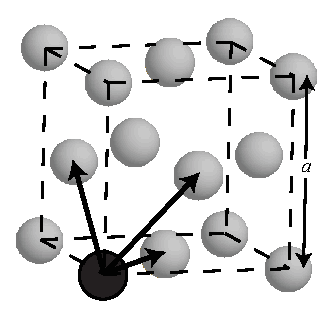
\includegraphics{/home/jason/thesis/thesis/table3-unitcell1.eps} 
% & Conventional (four atoms) 
% \newline 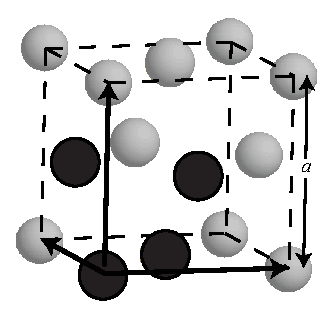
\includegraphics{/home/jason/thesis/thesis/table3-unitcell4.eps}\\ 
% \hline
% Basis& Face-centered Cubic & Simple Cubic\\ \hline
% Lattice Vectors& ($a/2$, $a/2$, 0), \newline ($a/2$, 0, $a/2$), 
% \newline (0, $a/2$, $a/2$)& ($a$, 0, 0), \newline (0, $a$, 0), 
% \newline (0, 0, $a$)\\ \hline
% Brillouin Zone& Truncated Octahedron \newline 
% 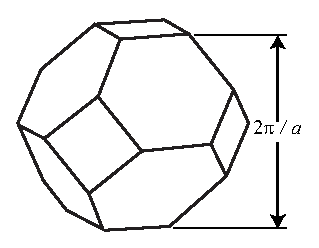
\includegraphics{/home/jason/thesis/thesis/table3-bz1.eps} & Cube \newline 
% 
\includegraphics{/home/jason/thesis/thesis/table3-bz4.eps}\\ \hline
% Number of \newline Wave Vectors& $N$ & $N/4$\\ \hline
% Polarizations/\newline Wave Vector& 3 & 12\\ \hline
% \hline
% \end{tabular}
% \end{center}
% \caption{The unit cell for a face-centered cubic crystal can be chosen 
% in different ways.}
% \label{T-unitcell}
% \end{table}
% \renewcommand{\baselinestretch}{2.0}
% %--------------------------------------------------------------------------
% 
% \clearpage
% 
% The selection of the unit cell sets the shape of the Brillouin zone and 
% the points that will be resolved inside it (i.e., the allowed wave 
% vectors, $\pmb{\kappa}$). For a simulation cell with $N$ atoms, there 
% are $3N$ normal modes. If the unit cell has one atom, there will be $N$ 
% allowed wave vectors, each with three polarizations (i.e., dispersion 
% branches, which we will denote by $\nu$). For a four-atom unit cell, 
% there will be $N/4$ allowed wave vectors, each with 12 polarizations. 
% In general, the choice of an $n$-atom unit cell will lead to $N/n$ 
% allowed wave vectors, each with 3$n$ polarizations. As such, there are 
% always $3N$ normal modes.
% 
% %--------------------------------------------------------------------------
% \subsection{\label{A:symmetry}Crystal Symmetries (WORK)}
% %--------------------------------------------------------------------------
% 
% Symmetry operations define the properties of a crystal. 
% This applies to any vector or tensor property of the crystal. The 
% symmetries do not depend on the unit cell represenation, although 
% conventional unit cells may have additional symmetries compared 
% to the primitive unit cells which is due to the redundant information of 
% using a conventional cell. 
% 
% Ab initio codes such as abinit and quantum espresso also print the 
% symmetry operations information. The 
% \href{http://spglib.sourceforge.net/}{spglib} 
% package contains a library of routines for utilizing the 
% symmetry operations of.
% 
% Contact Ankit Jain for more information on symmetry operations 
% and their application to thermal transport calculations. 
% 
% For the crystalline systems studied in Section , the wavevectors 
% are averaged over according to their symmetries, 
% which reduces the list of wavevectors to the first octant of the 
% cubic BZ.\cite{mcgaughey_phonon_2004} This reduction is equivalent 
% to applying roations of the 
% \href{http://en.wikipedia.org/wiki/Rotation_group_SO(3)}
% {SO(3) Group}, or the group of 90 degree rotations in Euclidean 
% (3-dimensional) space. 
% Any succesive combination of 90 degree roations is also a symmetry 
% operation. This property leads to the identity
% \begin{equation}\label{EQ:kpt_sym}
%  \begin{split}
%   \pmb{\kappa} = -\pmb{\kappa},
%  \end{split}
% \end{equation}
% which is the application of two 90 degree rotations, and is a 
% \href{http://en.wikipedia.org/wiki/Parity_(physics)#Odd}
% {general property of any crystal}. 
% 
% \href{https://github.com/jasonlarkin/disorder/blob/master/matlab/issym.m}
% {Here is a matlab function} which compares two vectors 
% and checks if they are related by any number of orthogonal 
% rotations.
% 
% For the LJ argon example, further reduction  of the wavectors is 
% possible by using all symmetry 
% \href{http://spglib.sourceforge.net/#rotation}{rotation operations} 
% of the 
% \href{http://www.wolframalpha.com/input/?i=face-centered+cubic}
% {face centered cubic lattice}. Additional 
% \href{http://en.wikipedia.org/wiki/Translational_symmetry}
% {translational symmetry operations} may exist. 
% For example, for the cubic conventional cell of LJ argon, translational 
% symmetries ensure that all four atoms in the unit cell are 
% equivalent. Thus, the conventional cell has more total 
% symmetries (rotational plus translational) than the primitive cell, 
% which is due to the redundant information contained within it. Similar 
% to conventional unit cells, crystalline supercells also have a larger 
% number of translational symmetries.
% 
% %--------------------------------------------------------------------------
% \subsection{\label{A:unitcell}Primitive, Conventional, and Supercell 
% Representations using Normal Mode Decomposition (WORK)}
% %--------------------------------------------------------------------------
% 
% Having described the normal mode decomposition theoretical approach and 
% computational methodology in Sections \ref{S-NMDformulation} and 
% \ref{S-workflow}, we now carry out a case study on a LJ crystal at a 
% dimensionless temperature of 0.0827 (corresponding to an argon 
% temperature of 10 K). While this temperature is low (the LJ argon Debye 
% temperature is around 85 K), it will allow for a clean demonstration of 
% the technique. The LJ interatomic potential is computationally inexpensive 
% and is thus ideal for use in code development and testing. All results 
% will be presented in dimensionless LJ units \cite{ashcroft_solid_1976}. 
% The zero pressure lattice constant is 1.556 (Ref. 
% \citenum{mcgaughey_phonon_2004}) 
% and the potential energy is cutoff and shifted at a distance of 2.5.
% 
% From the same simulation cell and atomic data, one can perform normal 
% mode decomposition on either the primitive or conventional unit cells.
% \footnote{The allowed wave vectors are defined by the basis
% and the supercell used to perform the MD simulations. For a supercell 
% built using the conventional unit cell, as we use, the allowed wave 
% vectors can be labeled using either the conventional or primitive unit 
% cell description.  For a supercell built using the primitive unit cell, 
% however, all wave vectors cannot be labeled using the conventional unit 
% cell description.} The [100] and [111] dispersion curves and density of 
% states obtained from harmonic lattice dynamics calculations are plotted 
% for each unit cell in Figs. \ref{F-dispersion}(a) and (b). While the 
% dispersion curves in each direction show similarities, they are 
% necessarily different due to the allowed wave vectors and shape of the 
% Brillouin zone (see Table \ref{T-unitcell}). The density of states, 
% however, are identical, as expected and required. We note that the 
% conventional unit cell description leads to what appear to be optical 
% modes. In reality, these modes are a result of zone folding and can be 
% mapped directly to acoustic modes in the primitive unit cell description.
% 
% The MD simulations are run in the $NVE$ ensemble, the dimensionless 
% time step is 0.002, and the equations of motion are integrated using 
% the velocity Verlet algorithm. The system is equilibrated for $2^{20}$ 
% time steps before collecting data every 25 time steps for an additional 
% $2^{20}$ time steps. In order to capture system-size effects, cubic 
% simulation cells with between 256 and 6912 atoms are considered 
% (corresponding to between four and twelve conventional unit cells, $N_0$, 
% in each of the $x$, $y$, and $z$ directions). Ten simulations are 
% performed with different initial velocities and the autocorrelations 
% (or Fourier transforms) are averaged over the initial conditions and 
% symmetric wave vectors before fitting the phonon properties.
% 
% \vspace{10mm}
% %\clearpage
% 
% \begin{figure}[t]
% \begin{center}
% \includegraphics[scale=1]
% {/home/jason/Dropbox/book/m_book_lj_disp_dos_vg_prim_novg-2.eps}
% \includegraphics[scale=1]
% {/home/jason/Dropbox/book/m_book_lj_disp_dos_vg_conv_novg-2.eps}
% \caption{\label{F-dispersion} {Dispersion curves and full Brillouin zone 
% density of states for a LJ crystal at a dimensionless temperature of 
% 0.0827. (a) [100] and [111] dispersion curves and density of states 
% based on the primitive (i.e., one atom) unit cell. (b) [100] and [111] 
% dispersion curves and density of states based on the conventional (i.e., 
% four atom) unit cell. The harmonic lattice dynamics calculations are 
% performed using a resolution of sixteen wave vectors along the reciprocal 
% lattice vectors of the conventional unit cell. The red and blue dots in 
% (b) are the modes considered in Fig. \ref{F-bulkfitting}.}}
% \end{center}\normalsize
% \vspace*{-0mm}
% \end{figure}
% 
% \vspace{10mm}
% \clearpage
% 
% The lifetimes predicted from the frequency-domain analysis for the 
% primitive and conventional unit cell representations of the $N_0=10$ 
% system are plotted in Fig. \ref{F-bulklifetimes}(a). The difference 
% between the lifetimes is less than 5\%, which is within the uncertainty 
% of the fitting. A $1/\omega^2$ scaling, predicted from theory for 
% phonon-phonon scattering at low frequencies \cite{callaway_model_1959}, 
% is plotted and is in good agreement with the trend in the data at low 
% frequencies. Also plotted is the Ioffe-Regel (IR) limit 
% \cite{taraskin_determination_1999},
% \begin{eqnarray}
% \tau_{IR} = \f{2 \pi}{\omega},
% \end{eqnarray}
% which corresponds to when the phonon lifetime is equal to its period. 
% All the modes in the perfect system have lifetimes well above this limit. 
% It is interesting to note that the phonon lifetimes do not decrease 
% monotonically with increasing frequency, with a maximum observed near 
% $\omega = 18$. Such a maximum is also observed in silicon lifetimes 
% obtained from the SW potential \cite{turney_-plane_2010} and from DFT 
% calculations \cite{esfarjani_heat_2011}.
% 
% \begin{figure}[t]
% \begin{center}
% \includegraphics[scale=1]
% {/home/jason/Dropbox/book/m_book_lj_nmd_prim_conv_compare-2.eps}
% \caption{\label{F-bulklifetimes} Lennard-Jones lifetimes from a 
% $N_0=10$ system at a temperature of 0.0827 predicted from normal mode 
% decomposition analysis on (a) the primitive and conventional unit 
% cells, and (b) treating the simulation cell as the unit cell (i.e., 
% Gamma-point analysis). All lifetimes extracted from time-domain analysis.}
% \end{center}\normalsize
% \end{figure}
% 
% \clearpage
% 
% In performing the normal mode decomposition, one is not limited to the 
% primitive or conventional unit cells. As needed for disordered systems 
% (see Sections \ref{S-alloy} and \ref{S-amorphous}) one can define the 
% simulation cell as the unit cell, such that all normal modes have 
% $\pmb{\kappa}=\mathbf{0}$ (i.e., they are all at the Gamma-point).
% \footnote{In Gamma-point analysis, all normal modes have zero group 
% velocity and it is not possible to predict mean free paths or thermal 
% conductivity.} The lifetimes for Gamma-point analysis for the same MD 
% data used to generate the lifetimes in Fig.\ref{F-bulklifetimes}(a)   
% are plotted in Fig.\ref{F-bulklifetimes}(b). The trends for the 
% Gamma-point analysis are the same as for the primitive and conventional 
% unit cells. There is more scatter in the Gamma-point data as wave 
% vector symmetry averaging is no longer possible.
% 
% The phonon properties obtained from normal mode decomposition and 
% harmonic lattice dynamics calculations can now be used to predict bulk 
% thermal conductivity using Eq.\eqref{E-kBTE}. For classical MD 
% simulations the assumption of equipartition of energy is very good and 
% we take the volumetric specific heat to be $k_\mathrm{B}/V$ for all 
% modes \cite{mcgaughey_quantitative_2004,goicochea_thermal_2010,
% larkin_comparison_2012}.
% 
% The Gamma point corresponds to bulk translation and therefore does not 
% contribute to thermal conductivity. By discretizing the Brillouin zone, 
% we assign a volume to the Gamma point. The zero contribution of this 
% volume to the thermal conductivity introduces a size effect in the 
% prediction. To predict a bulk thermal conductivity, an extrapolation 
% procedure is used, whereby $k$ is plotted versus $1/N_o$ and a line is 
% fit to the data. The point on this line where $1/N_o=0$ gives the bulk 
% thermal conductivity \cite{turney_predicting_2009,esfarjani_heat_2011}. 
% This extrapolation 
% procedure requires that the low-frequency modes be dominated by
% intrinsic scattering (i.e., $\tau \propto \omega^{-2}$) and have a 
% similar group velocity \cite{shiomi_thermal_2011,esfarjani_heat_2011}. 
% For the LJcrystal, this requirement is satisfied for modest system sizes
% ($N_0 \ge 6$). The size-dependent and extrapolated thermal conductivities 
% are plotted in Fig.\ref{F-bulksizeeffect} for both the primitive and 
% conventional unit cells. The Green-Kubo predictions for the same system 
% are also plotted and show no size effect, consistent with previous work 
% \cite{mcgaughey_quantitative_2004}.
% 
% % \begin{figure}[t]
% % \begin{center}
% % \includegraphics[scale=1.0]
% % {/home/jason/Dropbox/book/m_book_cond_extrap_c0-3_boxon.eps}
% % \caption{\label{F-bulksizeeffect} Size dependence of thermal conductivity 
% % for the LJ crystal at a temperature of 0.0827 from normal mode 
% % decomposition and the Green-Kubo method.}
% % \end{center}\normalsize
% % \vspace*{-0mm}
% % \end{figure}
% 
% The extrapolated thermal conductivities from the primitive and 
% conventional unit cells are $177 \pm 15$ and $176 \pm 14$ W/m-K. 
% The Green-Kubo thermal conductivity is $173 \pm 13$ W/m-K. All thermal 
% conductivities agree well within their respective uncertainties.
% 
% For the perfect LJ crystal, there is no clear advantage of performing 
% the analysis in the time or frequency domains or for the primitive or 
% conventional unit cells. Challenges may emerge for high thermal 
% conductivity materials like silicon or carbon nanotubes, where the 
% time-domain decay may not be well described by an exponential and the 
% peaks in frequency space get narrow or are not well-fit by a Lorentzian. 
% The failure of the fitting for a perfect crystal is an indication that 
% the relaxation time approximation may not be appropriate and that care 
% should be taken when interpreting the results. In general, new materials 
% should be investigated on a case-by-case basis to determine the approach 
% that minimizes the uncertainty.

%--------------------------------------------------------------------------
\section{\label{A:NMD XCORR}NMD using Non-Exact Normal Modes}
%--------------------------------------------------------------------------

In Chapter \ref{Chapter:SED}, it was shown how NMD is 
applied to a perfect crystal. In reality, any crystal will have some 
deviation from perfect periodicity, which may be caused by a point defect, 
a dislocation, a grain boundary, or a free surface. In extreme cases, 
these deviations from periodicity will lead to the emergence of modified 
normal modes. For small perturbations, however, it is reasonable to
assume that the frequencies and mode shapes of the normal modes will 
be unchanged and that the effect of the perturbation will be on the 
lifetimes. Under this assumption, one can still project the atomic 
positions and velocities onto the normal modes of the unperturbed system.

While one could perform the NMD by projecting 
the atomic positions and velocities onto the modes of the unperturbed 
system, it is more appropriate to use the virtual crystal approximation 
(Section \ref{S:From VC Gamma}). 
Under the virtual 
crystal approximation, the system is replaced by one where all atoms 
have the same mass, equal to the average of the atomic masses in the 
system of interest. This system will have the same mode shapes as the 
original system, but the frequencies are modified due to the change 
in the average atomic mass.

Results for the time- and frequency domain approaches to NMD 
are shown for two modes for crystalline and alloyed LJ argon in 
Figs. \ref{F-alloyfitting}(a)-(d). These two modes are equivalent to 
those shown in the perfect crystal in 
Figs. \ref{F-dispersion}(b), \ref{F-bulkfitting}(a), and 
\ref{F-bulkfitting}(b). For a concentration, $c$, of 0.05, both peaks 
in the frequency domain are well-formed and a lifetime can be extracted 
by fitting the data to a Lorentzian function. This behavior is typical 
of all modes at a concentration of 0.05. The downward frequency shift 
is related to the increased average atomic mass.

For an alloy concentration of 0.5, the lower frequency mode still has 
a well-formed peak. The higher-frequency mode does not, however, such 
that a lifetime cannot be extracted by fitting to a Lorentzian function. 
Such behavior is typical of the higher frequency modes at high alloy 
concentrations. This change in behavior is also seen in the time domain, 
where the decay of the autocorrelation of the total mode energy is no 
longer a smooth exponential function. This behavior indicates that the 
virtual crystal normal mode is not a good description of the true 
normal mode. Equation \eqref{E:tau_E_xcorr} can be used to approximate a 
lifetime, as shown in Figs. \ref{F-alloyfitting}(c) and 
\ref{F-alloyfitting}(d).

These artifacts observed using NMD method with the virtual crystal 
approximation are not surprising given two considerations: 
(i) the MD simulations 
contain explicit disorder that influences the atomic trajectories, 
and (ii) the VC-normal modes are not the exact normal modes of the 
explicitly-disordered lattice supercells. 
An effective lifetime can be predicted 
using Eq. \eqref{E:tau_E_xcorr} 
because the VC total mode energy autocorrelations 
still decay to zero in a finite time. This result is to be expected 
given that the atomic trajectories contain 
information about the lattice energy, which from general statistical 
physics principles will have exponential relaxation behavior in an 
equilibrium ensemble.
\cite{landau_statistical_1980,srivastava_physics_1990,
rajabpour_thermal_2010} The lifetimes predicted from the VC-NMD method 
are in reasonable agreement with those predicted from the Gamma-NMD 
method, which uses the exact normal modes of the disordered supercell 
(Section \ref{S:From VC Gamma}).  

% For a normal mode of the lattice supercell 
% used for the MD simulations (i.e., a Gamma mode), 
% the total energy autocorrelation is an exponential function  
% with a decay time $\tau\kv$ and the kinetic energy autocorrelation is a 
% exponentially-damped sinusoidal oscillation with frequency 
% $2\omega\kv$ (see Section \ref{S:Subsection_SED_time-domain}). 
% When projecting MD simulations  
% of the explicitly disordered lattice supercells 
% onto the VC normal modes, 
% the energy autocorrelation functions 
% do not always follow these simple functional forms, 
% as shown in Fig. \ref{F:NMD XCORR} for two modes in the LJ alloy at a 
% concentration of 0.5.  
% By calculating the mode kinetic energy in the  
% frequency-domain, $\Phi$,\cite{larkin_comparison_2012} artifacts such as 
% multiple peaks are observed (see main plot).   



% %--------------------------------------------------------------------------
% \begin{figure}
% \begin{center}
% \includegraphics[scale=1.0]
% {/home/jason/disorder/paper/vc/fig10.eps}
% \vspace*{-5mm}
% \end{center}
% \caption{\label{F:NMD XCORR} The normal mode kinetic energy, $\Phi$,  
% of two modes (A and B) at wavevector [0.25 0 0] calculated 
% using VC-NMD for a mass disordered LJ FCC supercell 
% ($N_0=8$ and $c=0.5$) is shown in the main figure. 
% The VC dispersion-predicted peaks are labeled 
% by $\omega_0$. The inset shows the same mode's energy 
% [kinetic ($KE$) and total ($TE$)] autocorrelation functions.  
% Note the additional oscillation effects in the KE and TE autocorrelation 
% functions for Mode B which are due to the two peaks in $\Phi$. 
% A mode lifetime can 
% be extracted unambiguously using the integral of the TE autocorrelation 
% function [Eq. \eqref{EQ:tau_nmd} in Section \ref{S:From VC Gamma}].}
% \end{figure}
% %--------------------------------------------------------------------------

%--------------------------------------------------------------------------
\begin{figure}[t]
\begin{center}
\includegraphics[scale=1]
{/home/jason/Dropbox/book/m_book_lj_disp_dos_vg_prim_novg-2.eps}
\includegraphics[scale=1]
{/home/jason/Dropbox/book/m_book_lj_disp_dos_vg_conv_novg-2.eps}
\caption{\label{F-dispersion} {Dispersion curves and full Brillouin zone 
density of states for a LJ crystal at a temperature of 
10 K. (a) [100] and [111] dispersion curves and density of states 
based on the primitive (i.e., one atom) unit cell. (b) [100] and [111] 
dispersion curves and density of states based on the conventional (i.e., 
four atom) unit cell. The harmonic lattice dynamics calculations are 
performed using a resolution of sixteen wave vectors along the reciprocal 
lattice vectors of the conventional unit cell. The red and blue dots in 
(b) are the modes considered in Fig. \ref{F-bulkfitting}.}}
\end{center}\normalsize
\vspace*{-0mm}
\end{figure}
%--------------------------------------------------------------------------

%--------------------------------------------------------------------------
\begin{figure}
\begin{center}
\includegraphics[scale=1.0]
{/home/jason/Dropbox/book/m_book_lj_nmd_xcorr_compare_c0_c05_c5_sed.eps}
\includegraphics[scale=1.0]
{/home/jason/Dropbox/book/m_book_lj_nmd_xcorr_compare_c5_xcorr.eps}
\end{center}
\caption{\label{F-alloyfitting} 
Virtual crystal (a) frequency-domain 
and (b) time-domain NMD analysis for two modes 
in LJ alloys with concentrations of 0.05 and 0.5. For modes that are 
not well-approximated by the virtual crystal modes, the lifetime can 
be approximated using Eq. \eqref{E:tau_E_xcorr}, as shown in (d).
}
\end{figure}
%--------------------------------------------------------------------------
\vspace{5mm}
\clearpage

%--------------------------------------------------------------------------
\section{\label{A:metastability}Effect of Metastability for 
Amorphous Solids on Normal Mode Decomposition}
%--------------------------------------------------------------------------

Amorphous materials may have many different atomic 
configurations with nearly equivalent potential energies, 
leading to potential metastability during MD simulations 
\cite{buchenau_structural_1988,feldman_numerical_1999,
durandurdu_<i>ab_2002,bernstein_structural_2006,he_heat_2011}. 
This meta-stability can 
cause errors when predicting vibrational lifetimes using NMD, 
which is demonstrated below. 

This case study is performed on an amorphous LJ system with 2048 atoms 
at a temperature of 5 K. 
The amorphous solid is generated by liquefying the 
crystal, instantaneously removing all kinetic energy, and then relaxing 
the structure (i.e., a melt-quench, Sections \ref{S:Calculation} 
and \ref{S:Sample}). 
The MD simulation parameters are the same as for the 
LJ crystal and alloy (Section \ref{S:Calculation}). 
The LJ 
amorphous phase is metastable at this temperature and intermittently 
moves between very similar low-energy states. Evidence for the 
metastability can be found by analyzing the time-histories of the atomic 
displacements. As such, NMD, which requires the 
average atomic positions, will be an approximation.

The time- and frequency-domain approaches to NMD 
are shown for two mode in the amorphous system in 
Figs. \ref{F-amorphousfitting}(a) and \ref{F-amorphousfitting}(b). 
Because the analysis is performed at the Gamma-point, the peaks are 
well formed, but they are not Lorentzian. 
The oscillations in the total energy 
correlation for the low frequency mode is a consequence of the 
metastability of the amorphous phase. As such, the lifetimes are extracted 
by using Eq. \eqref{E:tau_E_xcorr}, as shown in the inset to 
Fig. \ref{F-amorphousfitting}(b). 
The lifetimes for the amorphous system are plotted in 
Fig. \ref{F-amorphouslifetimes}. Compared to the crystal, the lifetimes 
show little frequency dependence and a significant number at low 
frequencies fall below the IR limit [Eq. \eqref{EQ:IR}]. This result 
seems to be a consequence of the metastability, since this behavior 
is not observed for the NMD-predicted lifetimes for a-SiO$_2$ and a-Si 
(Fig. \ref{FIG:Lifetimes}, Section \ref{S:Life}), 
which were both annealed carefully to remove metastability 
(Section \ref{S:Sample}). Annealing the amorphous LJ system at the 
temperature studied does not remove metastability and leads to 
re-crystallization if performed for a long enough time ($>$ 5 ns). 

\begin{figure}[t]
\begin{center}
\includegraphics[scale=0.85]
{/home/jason/Dropbox/book/m_nmd_xcorr_fit_lj_plot-2.eps}
\caption{\label{F-amorphousfitting} (a) Time-domain and (b) frequency 
domain NMD analysis for two modes in an amorphous 
LJ solid at a temperature of 10 K.}
\end{center}\normalsize
\vspace*{-5mm}
\end{figure}

\begin{figure}[h]
\begin{center}
\includegraphics[scale=0.85]
{/home/jason/Dropbox/book/m_lj_nmd_c0_amor_life.eps}
\caption{\label{F-amorphouslifetimes} Lifetimes predicted by normal 
mode decomposition for an amorphous LJ phase at a  
temperature of 5 K. The lifetimes for the crystal at a 
temperature of 10 K are provided for comparison.}
\end{center}\normalsize
\vspace*{-5mm}
\end{figure}

\clearpage

%--------------------------------------------------------------------------
\section{\label{Appendix_A:Finite}Finite Simulation-Size Scaling for 
Thermal Conductivity}
%--------------------------------------------------------------------------

The thermal conductivities predicted by the NMD ($\Phi$), 
$\Phi'$, 
VC-NMD, VC-ALD, and GK methods 
are system size-dependent [i.e., $k = k(N_0)$] for all lattices 
and amorphous materials methods except 
perfect LJ argon from GK\cite{mcgaughey_quantitative_2004} and 
a-SiO$_2$ (Section \ref{S:Bulk}). 
To predict a bulk thermal conductivity, $k_{bulk}$,  
a linear extrapolation procedure is 
used, whereby 
\begin{equation}\label{EQ:k0}
\frac{k(N_0)}{k_{bulk}} = 1 - \frac{c_0}{N_0},
\end{equation}
where $c_0$ is a constant \cite{turney_predicting_2009,
esfarjani_heat_2011,shiomi_thermal_2011,he_thermal_2011}. 
This procedure is necessary because the first 
Brillouin zone is only sampled at a finite number of points for a finite 
simulation size, with no contribution from the volume at its center. To 
predict a bulk thermal conductivity, it is important to sample points 
near the Brillouin zone center, where the modes can have large lifetimes 
and group velocities \cite{turney_predicting_2009,sellan_size_2010}. 

The thermal conductivity 
is predicted for varying system sizes and the bulk thermal conductivity 
is obtained by fitting Eq. \eqref{EQ:k0} to the data. 
For the NMD ($\Phi$), $\Phi'$, VC-NMD, and VC-ALD methods, 
the validity of Eq. \eqref{EQ:k0}  
requires that the low-frequency modes be dominated by 
phonon-phonon scattering (i.e., $\tau\ \propto \omega^{-2}$) and  
follow the Debye approximation 
with respect to the group velocity and DOS 
\cite{shiomi_thermal_2011,esfarjani_heat_2011}. For the LJ 
argon alloys, this requirement is satisfied for modest system sizes 
(for $N_0 = 6$ to $12$).


%--------------------------------------------------------------------------
% \begin{figure}
% \begin{center}
% \includegraphics[angle=0,width=80.0mm]
% {/home/jason/thesis/thesis/appendix/LJ_NMD_SED_COND_2.eps}
% \end{center}
% \caption{\label{F:LJ_COND} Thermal conductivity predictions for LJ argon 
% calculated using phonon lifetimes predicted by $\Phi$ and $\Phi'$. (a) 
% The finite simulation-size scaling extrapolation 
% \cite{turney_predicting_2009,he_thermal_2011} 
% is used to compare the results to bulk predictions made using the 
% Green-Kubo method. (b) The bulk results for $\Phi$ and Green-Kubo are 
% in good agreement temperatures of $20$ and $40$ K with those of other 
% atomistic simulation methods,\cite{turney_predicting_2009} while those 
% from $\Phi'$ differ (see Table \ref{T:cond_table}).}
% \end{figure}
%--------------------------------------------------------------------------
%\clearpage


% %--------------------------------------------------------------------------
% \section{\label{Appendix:AF}AF Calculations (WORK)}
% %--------------------------------------------------------------------------
% 
% 
% % https://github.com/jasonlarkin/disorder/blob/master/lj/alloy/af_di_compare_broadening.m
% 
% The AF theory suggests a broadening which is larger than the average 
% frequency spacing, $\delta_{avg}$. 
% 
% The role of energy broadening in MD simulations could be helpful. The 
% energy of a given mode is broadened for two reasons: 
% 
% 1) due to anharmonic interactions.
% 
% 2) due to disorder (i.e., phonon-defect scattering in alloys, 
% diffuson theory). 
% 
% The NMD-predicted lifetimes are predicted from MD simulations where 
% all scattering mechanisms are present. Based on the comparison 
% of NMD- and AF-predicted diffusivities in Fig. , a frequency-dependent 
% broadening may be necessary for the AF theory. The role of frequency 
% broadening needs further investigation. 
% 
% %--------------------------------------------------------------------------
% \subsection{\label{Appendix:AF:Physical}Physical Picture}
% %--------------------------------------------------------------------------
% 
% The AF theory makes the harmonic approximation. Physically, modes 
% couple by spatial and energetic (harmonic, elastic scattering) overlap.  
% The strength of the overlap is determined by how close the mode 
% energies (frequencies) are and how much the eigenvectors spatially overlap. 
% The two highest frequency modes of the LJ alloy at a concentration of 
% 0.5 (see Section , Fig. ) are shown in Fig. . The mode frequencies are 
% and . These modes are both highly localized locons, which is indicated 
% by the small amount of spatial overlap in the eigenvector components. Only 
% the two spatial-dimensional components of the total three 
% spatial-dimensional components of the eigenvectors are plotted. The 
% three dimensional atomic coordinates are plotted in two dimensions. 
% 
% %--------------------------------------------------------------------------
% \begin{figure}
% \begin{center}
% \includegraphics[angle=0,width=80.0mm]
% {/home/jason/disorder/lj/alloy/m_eig_3d_plot_lj_alloy_c5_mode11999_12000.eps}
% \end{center}
% \caption{\label{F:LJ_COND} Spatial components of the eigenvectors of two 
% locons. The spatial localization is evident from the small amount of 
% spaital overlap of the mode eigenvectors.}
% \end{figure}
% %--------------------------------------------------------------------------
% 
% \clearpage
% 
% %--------------------------------------------------------------------------
% \subsection{\label{Appendix:AF:Finite}Finite Size Effects}
% %--------------------------------------------------------------------------
% 
% 
% % Hi Julian,
% % 
% % No problem about the silence, I have been busy trying to wrap up my thesis and find a job!
% % 
% % So, here are the issues:
% % 
% % 1) On the journey back from the most recent trip I was reading though the draft
% % manuscript that you sent me & puzzling over the issue of the size / Lorentzian sensitivity
% % of the answers.
% % 
% % Yes, this is kind of a tricky part of the AF method.  It seems like this was never addressed in the 
% % main paper, they simply suggest using a broadening equal to the average frequency spacing,\cite{feldman_thermal_1993} 
% % which is continued in \cite{feldman_numerical_1999} and \cite{shenogin_thermal_2009}. 
% % It turns out that the frequency spacing \delta_{freq} is strongly freq dependent, especially at low frequencies where the modes 
% % are sparse. Here is a crude plot for an a-LJ sample:
% % 
% % https://github.com/jasonlarkin/disorder/blob/master/lj/alloy/af_di_dw_amor.png
% % 
% % This has different effects depending on the system.  
% % 
% % For LJ alloys, the k_{AF} is strongly system-size dependent:
% % 
% % https://github.com/jasonlarkin/disorder/blob/master/lj/alloy/af_k_kmax.png
% % 
% % This is due to the harmonic approximation used in the AF theory, which leads to a Rayleigh scaling of 
% % the low-freq modes, \tau\propto\omega^{-4}. Here is another crude plot, showing the \omega^{-4} scaling 
% % predicted
% % 
% % https://github.com/jasonlarkin/disorder/blob/master/lj/alloy/af_di_all.png
% % 
% % While a-LJ shows a dependence on the broadening,  (\bra{\delta}=x*\delta_{avg} in this figure). Amorphous LJ is equivalent to a disordered lattice with a large disorder parameter.\cite{beltukov_ioffe-regel_2013}
% % 
% % 
% % The effect on a-Si is more complicated. For broaden = \delta_{avg}, the diffusivities at low frequency 
% % have large fluctuations. No definitive scaling can be seen, there seems to be a mix of \omega^{-4} and \omega^{-2} scalings. 
% % 
% % By increasing the broadening, the low frequency scaling can be tuned to match \omega^{-2} or \omega^{-4}:
% % 
% % https://github.com/jasonlarkin/disorder/blob/master/si/amor/m_af_si_normand_N0_3.png
% % 
% % The low-frequecy fluctuations can be smoothed by increasing the broadening over a small range:
% % 
% % https://github.com/jasonlarkin/disorder/blob/master/si/amor/m_af_si_normand_N0_5.png
% % 
% % This exaplins why Shenogin et al.'s prediction of k_{AF} = 1.0 W/m-K for a 512 atom system:
% % 
% % https://github.com/jasonlarkin/disorder/blob/master/si/amor/m_af_feldman_shenogin_fabian.png
% % 
% % which is due to using a small broadening. 
% % 
% % 
% % 
% % 
% % 
% % 
% % 1) I'm not quite clear on is what the final result is for the K_ph contribution that has to be
% % added. I realise that this was an early draft since all the cross referencing etc wasn't 
% % finished, and so perhaps you have an updated version that might help?
% % 
% % Ya sorry, that was a pretty early draft.  Here is the one which is just about to be submitted:
% % 
% % https://github.com/jasonlarkin/disorder/raw/master/paper/mfp/prb_mfp_jl_081613.pdf
% 
% %--------------------------------------------------------------------------
% % \begin{figure}
% % \begin{center}
% % \includegraphics[bb=0 0 3cm 3cm]
% % {/home/jason/disorder/lj/alloy/af_di_all.png}
% % \end{center}
% % \caption{\label{F:LJ_COND} Spatial components of the eigenvectors of two 
% % locons. The spatial localization is evident from the small amount of 
% % spaital overlap of the mode eigenvectors.}
% % \end{figure}
% % %--------------------------------------------------------------------------
% % 
% % 
% % %--------------------------------------------------------------------------
% % \begin{figure}
% % \begin{center}
% % \includegraphics[bb=0 0 3cm 3cm]
% % {/home/jason/disorder/lj/alloy/af_di_dw_0.05.png}
% % \includegraphics[bb=0 0 3cm 3cm]
% % {/home/jason/disorder/lj/alloy/af_di_dw_amor.png}
% % \end{center}
% % \caption{\label{F:LJ_COND} Spatial components of the eigenvectors of two 
% % locons. The spatial localization is evident from the small amount of 
% % spaital overlap of the mode eigenvectors.}
% % \end{figure}
% % %--------------------------------------------------------------------------
% % 
% % %--------------------------------------------------------------------------
% % \begin{figure}
% % \begin{center}
% % \includegraphics[bb=0 0 3cm 3cm]
% % {/home/jason/disorder/lj/alloy/af_di_kappa(broaden).png}
% % \end{center}
% % \caption{\label{F:LJ_COND} Spatial components of the eigenvectors of two 
% % locons. The spatial localization is evident from the small amount of 
% % spaital overlap of the mode eigenvectors.}
% % \end{figure}
% % %--------------------------------------------------------------------------
% % 
% % %--------------------------------------------------------------------------
% % \begin{figure}
% % \begin{center}
% % \includegraphics[bb=0 0 3cm 3cm]
% % {/home/jason/disorder/lj/alloy/af_k_kmax.png}
% % \end{center}
% % \caption{\label{F:LJ_COND} Spatial components of the eigenvectors of two 
% % locons. The spatial localization is evident from the small amount of 
% % spaital overlap of the mode eigenvectors.}
% % \end{figure}
% %--------------------------------------------------------------------------



% %--------------------------------------------------------------------------
% \section{\label{Appendix:SF}Spectral Density of Disordered Modes (WORK)}
% %--------------------------------------------------------------------------
% 
% %--------------------------------------------------------------------------
% % \begin{figure}
% % \begin{center}
% % \includegraphics[bb=0 0 3cm 3cm]
% % {/home/jason/disorder/lj/alloy/dsf_alloy_0.5_mode100.png}
% % \includegraphics[bb=0 0 3cm 3cm]
% % {/home/jason/disorder/lj/alloy/dsf_alloy_0.5_mode3000.png}
% % \includegraphics[bb=0 0 3cm 3cm]
% % {/home/jason/disorder/lj/alloy/dsf_alloy_0.5_mode4000.png}
% % \end{center}
% % \caption{\label{F:LJ_COND} Spatial components of the eigenvectors of two 
% % locons. The spatial localization is evident from the small amount of 
% % spaital overlap of the mode eigenvectors.}
% % \end{figure}
% %--------------------------------------------------------------------------
% 
% 
% %--------------------------------------------------------------------------
% \section{\label{Appendix:Accum}Size-effects for Low-frequency Dominated 
% Materials (WORK)}
% %--------------------------------------------------------------------------
% 
% %--------------------------------------------------------------------------
% \begin{figure}
% \begin{center}
% \includegraphics[angle=0,width=80.0mm]
% {/home/jason/disorder/si/alloy/m_ald_taud_si_cond_N0_ald_gk_nmd.eps}
% \end{center}
% \caption{\label{F:LJ_COND} Spatial components of the eigenvectors of two 
% locons. The spatial localization is evident from the small amount of 
% spaital overlap of the mode eigenvectors.}
% \end{figure}
% %--------------------------------------------------------------------------
% 
% \clearpage
% 
% %--------------------------------------------------------------------------
% \section{\label{Appendix:Accum}Accumulation Functions in Alloys 
% (WORK)}
% %--------------------------------------------------------------------------
% 
% 
% %--------------------------------------------------------------------------
% \begin{figure}
% \begin{center}
% \includegraphics[angle=0,width=80.0mm]
% {/home/jason/disorder/lj/alloy/m_ald_taud_lj_kaccum.eps}
% \end{center}
% \caption{\label{F:LJ_COND} Spatial components of the eigenvectors of two 
% locons. The spatial localization is evident from the small amount of 
% spaital overlap of the mode eigenvectors.}
% \end{figure}
% %--------------------------------------------------------------------------
% 
% \clearpage
% 
% %--------------------------------------------------------------------------
% \begin{figure}
% \begin{center}
% \includegraphics[angle=0,width=80.0mm]
% {/home/jason/disorder/lj/alloy/xcorr_alloy_cum_cond.eps}
% \end{center}
% \caption{\label{F:LJ_COND} Spatial components of the eigenvectors of two 
% locons. The spatial localization is evident from the small amount of 
% spaital overlap of the mode eigenvectors.}
% \end{figure}
% %--------------------------------------------------------------------------
% 
% \clearpage
% 
% %--------------------------------------------------------------------------
% \begin{figure}
% \begin{center}
% \includegraphics[angle=0,width=80.0mm]
% {/home/jason/disorder/si/alloy/m_ald_taud_si_klambda.eps}
% \end{center}
% \caption{\label{F:LJ_COND} Spatial components of the eigenvectors of two 
% locons. The spatial localization is evident from the small amount of 
% spaital overlap of the mode eigenvectors.}
% \end{figure}
% %--------------------------------------------------------------------------
% 
% \clearpage
% 
% %--------------------------------------------------------------------------
% \begin{figure}
% \begin{center}
% \includegraphics[angle=0,width=80.0mm]
% {/home/jason/disorder/si/alloy/m_ald_taud_si_cond_N0_ald_gk_nmd.eps}
% \end{center}
% \caption{\label{F:LJ_COND} Spatial components of the eigenvectors of two 
% locons. The spatial localization is evident from the small amount of 
% spaital overlap of the mode eigenvectors.}
% \end{figure}
% %--------------------------------------------------------------------------
% 
% \clearpage




%--------------------------------------------------------------------------
\chapter{Research using High Performance Computing}
%--------------------------------------------------------------------------

%--------------------------------------------------------------------------
\section{Setting Up Computing Environment}
%--------------------------------------------------------------------------


%%--------------------------------------------------------------------------
%\subsection{Suggested Reading}
%%--------------------------------------------------------------------------


%The online encyclopedia \href{http://www.wikipedia.org/}{wikipedia} 
%has become an excellent resource for technical knowledge. 

%\href{http://en.wikipedia.org/wiki/Statistical_mechanics}
%{Statistical Mechanics}/
%\href{http://en.wikipedia.org/wiki/Condensed_matter}
%{Condensed Matter}
%\cite{ashcroft_solid_1976,mcquarrie_statistical_2000}

%\href{http://en.wikipedia.org/wiki/Phonon}
%{Lattice Dynamics} with focus on the classical, quantum 
%and thermodynamic properties of phonons.\cite{peierls_,ziman,
%wallace_thermodynamics_1976,
%srivastava_1990,dove_lattice_1993} 

%\href{http://en.wikipedia.org/wiki/Introduction_to_quantum_mechanics}{Introduction to quantum mechanics and quantum chemistry}
%\cite{griffiths_introduction_1995} 
%and more 
%advanced topics on 
%\href{https://en.wikipedia.org/wiki/Electron_configuration}
%{Electron Strucutre} and 
%\href{http://en.wikipedia.org/wiki/Density_functional_theory}
%{Density Functional Theory}.
%\cite{martin_electronic_2004} 

%Analytical methods for 
%\href{http://en.wikipedia.org/wiki/Ordinary_differential_equations}
%{ordinary} and 
%\href{http://en.wikipedia.org/wiki/Partial_differential_equation}
%{partial differential equations}, 
%\href{http://en.wikipedia.org/wiki/Fourier_analysis}
%{fourier} and 
%\href{http://en.wikipedia.org/wiki/Statistics}
%{statistical analysis},\cite{mcquarrie_mathematical_2003} 
%and 
%\href{http://en.wikipedia.org/wiki/Numerical_analysis}
%{numerical analysis}.\cite{moin_fundamentals_2010} For example, 
%the LJ MD code discussed in Section uses a  
%\href{http://en.wikipedia.org/wiki/Verlet_integration}
%{verlet integration method}. 

%--------------------------------------------------------------------------
\subsection{Hardware and Operating System Choice}
%--------------------------------------------------------------------------

The choice of hardware determines the operating system. The three 
main choices for operating system are Windows, Apple OS, and Linux. Each 
operating system has limitations depending on the hardware it 
operates on.   
For example, Apple OS is primarily used on Apple hardware.

\href{http://www.youtube.com/watch?v=7XTHdcmjenI}
{Linux: world's most widely used software}
Linux runs on cell phones to the world's largest supercomputers. 
Reccomend the most widely used linux version 
\href{http://www.ubuntu.com/}{ubuntu}.
well-documented, large-community discussion
Apple OS is an adequate substitute as it is 
\href{https://en.wikipedia.org/wiki/Unix-like}{unix-like}.

There are many options for installing Ubuntu and the instructions 
can be found on \href{http://www.ubuntu.com/}{http://www.ubuntu.com/}.
Ubuntu is certified on 
\href{http://www.ubuntu.com/certification/}
{many top PC's from many computer companies}
and a company, \href{https://www.system76.com/}{system 76}, 
builds computers with Ubuntu pre-installed. I used the 
\href{https://www.system76.com/laptops/model/panp9}
{Pangolin Performance} for over a year of my PhD.  However, 
I reccomend using the lightest, most-portable, and longest-battery 
life notebook available such as the 
\href{https://help.ubuntu.com/community/SamsungSeries9}
{Samsung Series 9}  
or \href{https://help.ubuntu.com/community/MacBookAir}{Macbook Air}. 
You will typically be using this notebook to access large computing 
clusters remotely, 
so there is a benefit of having portability and long 
battery life over large computational power.  

%--------------------------------------------------------------------------
\subsection{System Terminal and Commands}
%--------------------------------------------------------------------------

These instructions work best for Ubuntu operating system, and will work 
well for other versions of Linux. Systems commands are executed by the 
system 
\href{https://help.ubuntu.com/community/UsingTheTerminal}{terminal}. 


Useful Linux Commands:

sed, grep, ls, cd, pwd, export, setenv, scp -r, ssh, sudo, nohup, 
vi, cat, which, echo

\href{https://www.google.com/search?q=linux+sed}
{google: linux sed} 

%--------------------------------------------------------------------------
\subsection{Environment Variables}
%--------------------------------------------------------------------------

\href{http://en.wikipedia.org/wiki/Environment_variable}
{environment variable} such as $\$$PATH.  Here is how we determine what 
PATH is set to:


Set PATH for lammps (see Section ).


Permanent changes to environment variables can be made in the user's 
.bashrc file, which is typically located in the /home/user/ directory. 
The .bashrc file is a hidden file noted by its name starting with ".". 
Other

Here is an example .bashrc which demonstrates how to add permanent paths 
and how to define new functions within the operating system. 
For example, to copy the output of the pwd command to the system's 
clipboard, use cpyc then "ctrl-v" elsewhere. 

This file modifies environment variables such as 
\href{https://help.ubuntu.com/community/EnvironmentVariables}{PATH}  
when a bash terminal session is launched. Changes to environment 
variables are made when a new terminal session is started. The 
location of this file is typically: /home/user/.bashrc.  The 

\href{https://gist.github.com/kparrish/6064111}{.bashrc} from 
Kevin Parrish.

%--------------------------------------------------------------------------
\subsection{Shell Scripts and System Commands in Python}
%--------------------------------------------------------------------------

Shell scripts are relatively low-level scripts which execute system 
commands (Section ) and 
manipulate environment variables (Section )   
of the Linux operating system. 

Here is a simple tutorial on writing shell scripts 
\href{http://linuxcommand.org/wss0010.php}
{http://linuxcommand.org/wss0010.php}

Running Linux system commands in Python can be an effective way of 
generating and manipulating many files with one script. Python 
is a more robust language than lower-level shell scripting. 
Here is an example:

lmp.in.iseed

%--------------------------------------------------------------------------
\subsection{Remote Resources Commands}
%--------------------------------------------------------------------------

At some point during research you will need to excecute code on remote 
resources which are typically large ($\gt 100$ cpu) computing clusters. 
You will be provided with a terminal session similar to the session 
provided by Ubuntu with most of the same system commands. 

While I recommend 
\href{https://filezilla-project.org/}{Filezilla} 
for handling the transfer of data and files, 
the functionality of Filezilla is contained in several shell 
commands:

ssh user@gilgamesh.cheme.cmu.edu

or equivalently by the machine's ip address:

ssh user@xxx.xxx.xxx.xxx

Files can be transferred using the following command:

scp -r user@gilgamesh.cheme.cmu.edu:/home/user/directory/ ./

which will place the "directory" and its contents into the pwd (./) 
of the local terminal session. 

There are many variants of the operating systems used for remote 
computing clusters, but the differences are usually superficial. 
During my work I used the 
\href{http://gilgamesh.cheme.cmu.edu/doc/gilgamesh.html}
{gilgamesh} computing cluster maintained by 
\href{https://github.com/jkitchin}{John Kitchin}. 
\href{http://gilgamesh.cheme.cmu.edu/doc/gilgamesh.html}
{Gilgamesh's documentation} is a good resource for learning how to run 
calculations on a computing cluster.

%--------------------------------------------------------------------------
\subsection{Installing Programs}
%--------------------------------------------------------------------------

Ubuntu and similar linux OS have automatic software installation and 
management using the apt-get system command:

jason@jason-900X3C ~/ (master) $\$$ sudo apt-get install gfortran
[sudo] password for jason: 
Reading package lists... Done
Building dependency tree       
Reading state information... Done
gfortran is already the newest version.
The following package was automatically installed and is no longer required:
  kde-l10n-engb
Use 'apt-get autoremove' to remove it.
0 upgraded, 0 newly installed, 0 to remove and 129 not upgraded.

To check that the package has been installed, use:

jason@jason-900X3C-900X3D-900X3E-900X4C-900X4D ~/ (master) $\$$ which gfortran
/usr/bin/gfortran

This shows that gfortran program is installed in the /usr/bin/ folder, 
a common location where automatically installed programs are located. 
Because the 
folder /usr/bin is in the PATH environment variable:


the program gfortran is always available no matter where you are in 
the system terminal. 

To get more information about the gfortran, use:

jason@jason-900X3C ~/ (master) $\$$ ls -l /usr/bin/gfortran
lrwxrwxrwx 1 root root 12 Apr 22 03:44 /usr/bin/gfortran -> gfortran-4.7

where we see that /usr/bin/gfrotran "points" to gfortran-4.7. 
This is called a symbolic link, which can be created using:

jason@jason-900X3C ~/disorder/pcbm/topotools-tutorial-part2 (master) $\$$ ls -l /usr/bin/gfortran
lrwxrwxrwx 1 root root 12 Apr 22 03:44 /usr/bin/gfortran -> gfortran-4.7

%--------------------------------------------------------------------------
\subsection{Available Programs}
%--------------------------------------------------------------------------

Available progams represent oppurtunities to perform research quickly and 
easily. I suggest you read their documentation carefully and try the 
tutorials which are typically computationally inexpensive. 

Install lammps:

Set PATH for lammps

gnu compilers vs intel: gnu freely available
tar -zxvf lammps.tar, make serial, sudo apt-get install openmpi, make openmpi

open-source: 

\href{http://lammps.sandia.gov/}{LAMMPS}, including the particularly 
useful 
\href{http://lammps.sandia.gov/threads/threads.html}{mailing list} 
(use ctrl-f to search on any topic)  
and
\href{http://lammps.sandia.gov/doc/Section_python.html}
{python interface} which is used with the package 
\href{http://github.com/ntpl/ntpy}{ntpy}. 
\href{http://projects.ivec.org/gulp/}{GULP}, 
\href{http://www.abinit.org/}{ABINIT}, 
\href{http://www.quantum-espresso.org/}{Quantum Espresso}, 
\href{http://jp-minerals.org/vesta/en/}{VESTA}, 
\href{http://phonopy.sourceforge.net/}{phonopy}, 
\href{http://www.ks.uiuc.edu/Research/vmd/}{VMD} 
(with 
\href{https://sites.google.com/site/akohlmey/software/topotools}
{topotools})
\href{http://github.com/ntpl/ntpy}{ntpy},
\href{https://www.vasp.at/}{VASP}
\href{http://www.stfc.ac.uk/CSE/randd/ccg/software/DL_POLY/25526.aspx}
{DL_POLY}, 
\href{http://icmab.cat/leem/siesta/}
{siesta}, 
\href{http://www.msg.ameslab.gov/gamess/}{GAMESS}, 
\href{http://www.cp2k.org/}{CP2K}, 
\href{http://www.icams.de/content/departments/ams/madsen/boltztrap.html}{BOLTZTRAP}, 
\href{http://www.homepages.ucl.ac.uk/~ucfbdxa/phon/}{PHON}, 

I reccomend trying this 
\href{https://gist.github.com/kparrish/6064159}{install.sh} created by 
\href{http://www.github.com/kparrish}{Kevin Parrish} which installs 
many programs and packages, including lammps for parallel computing 
with openmpi.

%--------------------------------------------------------------------------
\section{Preparing Journal Articles and Thesis}
%--------------------------------------------------------------------------

reccomendation: student advisor should try and exchange editing a written 
research documen at least every week. The exchange of such a document 

Such a research document could be the running 
collection of journal articles which turn into the thesis. Maintenance 
of this document can be achieved with 
\href{https://www.dropbox.com/}{Dropbox} or 
Github. 
Github offers to advantage of smart version control and a built-in 
wiki. 



%--------------------------------------------------------------------------
\subsection{Journal Articles}
%--------------------------------------------------------------------------

The job of the student is to prepare, submit, and publish 
peer-reviewed journal articles. There are many journals suitable for 
nanoscale transport topics. All of them accept 
\href{http://www.latex-project.org/}{Latex} prepared manuscripts. 
I recommend the Latex editor 
\href{http://kile.sourceforge.net/}{Kile}, while the simple 
\href{https://projects.gnome.org/gedit/}{gedit} works well and comes 
pre-installed with Ubuntu. Here is a 
\href{http://mally.stanford.edu/~sr/computing/latex-example.html}
{simple latex example} and how to generate a 
\href{http://tex.stackexchange.com/questions/1596/how-to-compile-a-latex-document}
{portable document format (PDF)} from the latex document.  

To maintain the reference library I 
recommend 
\href{http://www.zotero.org/}{zotero}.  Here is an example 
\href{}{reference.bib} 
file which is exported automatically by zotero. 
The references are generated from the latex document using 
\href{http://www.bibtex.org/Using/}{bibtex} which compiles the contents of 
the reference.bib.

Here is an example of the latex files 
used to create an article published from this work:

\href{https://github.com/jasonlarkin/thesis/tree/master/thesis}
{Predicting alloy properties}.

This file uses 
\href{http://publish.aps.org/revtex}{revtex}, 
which is an article class used by Physical Review, 
Journal of Applied Physics, and others.

%--------------------------------------------------------------------------
\subsection{Thesis}
%--------------------------------------------------------------------------

These can be used as templates

Here is a Carnegie Mellon thesis template:

\href{https://github.com/robsimmons/cmu-thesis}
{https://github.com/robsimmons/cmu-thesis}

\href{https://github.com/jasonlarkin/thesis/tree/master/thesis}
{J. Larkin thesis files}.

\href{http://web.science.mq.edu.au/~rdale/resources/writingnotes/latexstruct.html}
{Article on structuring large documents.}

%2) Computational cost of each paper
%CPU, memory
%parallel cpu, parallel memory
%Trends: 
%small single cpu jobs -> large parallel cpu jobs
%single predictive method -> several predictive methods
%reccomendation: explore all predictive methods and models possible

%--------------------------------------------------------------------------
\section{Technical Advice}
%--------------------------------------------------------------------------

In addition to your advisor and close mentors, 
I reccomend communicating with experts in the field as much as 
possible without being an annoying.  How often to 
communicate depends on the situation. 
It is best to let the expert dictate the pace of the conversation. 

%--------------------------------------------------------------------------
\subsection{Expert Advice}
%--------------------------------------------------------------------------

Here is a list of experts I used as resources for this work. They 
will typically answer emails within 24-48 hours:


\href{http://ntpl.me.cmu.edu/people.html}
{Alan McGaughey},
\href{http://www.cmu.edu/me/malen/Lab_Website/People.html}
{Jon Malen},
\href{http://chemistry.curtin.edu.au/people/academic.cfm/J.Gale}
{Julian Gale} 
\href{http://projects.ivec.org/gulp/news.html}
{(GULP author)},
\href{http://mech.rutgers.edu/content/keivan-esfarjani}
{Keivan Esfarjani},
normand.mousseau@umontreal.ca,
guido.raos@polimi.it,
\href{mailto:joseph.feldman.ctr@nrl.navy.mil}
{Joseph Feldman},
\href{http://www.phonon.t.u-tokyo.ac.jp/}
{Junchiro Shiomi},
\href{http://www2.mpip-mainz.mpg.de/~donadio/tnt/People.html}
{Davide Donadio},
\href{http://www.ce.cmu.edu/people/faculty/maloney.html}
{Craig Maloney},
\href{http://quasiamore.mit.edu/pmwiki.php?n=Main.JivteshGarg}
{Jivtesh Garg},
\href{John Duda}
{John Duda},
\href{Wissam Al-Saidi}
{Wissam Al-Saidi},
\href{Dan Sellan}
{Dan Sellan},
\href{Ankit Jain}
{Ankit Jain},
\href{wong@andrew.cmu.edu}
{Wee-Liat Ong},
\href{John Kitchin}
{John Kitchin},
Steve Plimpton via the 
\href{http://lammps.sandia.gov/threads/threads.html}{LAMMPS mailing list} 
Axel Kolhmeyer via the 
\href{http://lammps.sandia.gov/threads/threads.html}{LAMMPS mailing list} 
and \href{akohlmey@gmail.com}{email}

\href{http://atztogo.users.sourceforge.net/}{Atz Togo}, creator of 
\href{http://phonopy.sourceforge.net/}{phonopy}

\href{http://jasonlarkin.github.io}{me}

%--------------------------------------------------------------------------
\subsection{Online Resources}
%--------------------------------------------------------------------------

wikipedia

\href{http://www.sklogwiki.org/SklogWiki/index.php/Main_Page}
{octave}

https://en.wikipedia.org/wiki/Lennard-Jones_potential

http://www.sklogwiki.org/SklogWiki/index.php/Lennard-Jones_model

we can do better, needs to be organization. 

http://nanohub.org/

does not provide good HPC resources. 


%--------------------------------------------------------------------------
\section{Coding Languages: Compiled versus Interpreted}
%--------------------------------------------------------------------------

There are many languages 
used for the open-source and lisenced packages(REF) that can be used 
to study nanoscale transport. These packages use 
\href{http://en.wikipedia.org/wiki/Compiled_language}{compiled} and 
\href{http://en.wikipedia.org/wiki/Interpreted_language}{interpreted}  
languages and often a miture of the two.

The most commonly used compiled languages are 
\href{https://en.wikipedia.org/wiki/C\%2B\%2B}{C/C++} 
(linux, LAMMPS) 
and 
\href{http://en.wikipedia.org/wiki/Fortran}{Fortran}
(GULP, quantum espresso, VASP).

A good discussion on 
\href{http://stackoverflow.com/questions/13078736/fortran-vs-c-does-fortran-still-hold-any-advantage-in-numerical-analysis-thes}
{the strengths of C++ versus Fortran}.

\href{http://www.youtube.com/watch?v=XFQ9dw3CyDo&list=PL1D10C030FDCE7CE0}
{excellent c++ tutorial}

\href{http://www.youtube.com/watch?v=YRTEOFMUTzw&list=PL6A8E21D2E86A0155}
{excellent fortran tutorial}


The two interpreted languages you are likely to use are 
\href{http://en.wikipedia.org/wiki/MATLAB}{matlab}  
and 
\href{http://en.wikipedia.org/wiki/Python_(programming_language)}{python}.

The key to maximizing the potential of interpreted languages is by 
using the built-in ``vector'' functions and operations provided by the 
\href{http://www.mathworks.com/help/matlab/matlab_prog/vectorization.html}
{matlab}  
and 
\href{http://faculty.washington.edu/rjl/uwamath583s11/sphinx/notes/html/python_vect.html}
{python}  
programming libraries.

matlab has an excellent built-in guide, google search will typically 
yield useful results. A good open-source substitute for matlab is 
\href{http://www.gnu.org/software/octave/}
{octave} which is capable to running most matlab scripts.

%--------------------------------------------------------------------------
\subsection{Compiled Language Case-study: Lennard-Jones Argon Molecular Dynamics}
%--------------------------------------------------------------------------

The first case study is a 
\href{https://github.com/jasonlarkin/classes/tree/master/cmu/molecular_simulation/HW5}
{single C code to perform Molecular Dynamics 
on LJ argon}. The code is a serial code with 

/home/jason/classes/cmu/molecular_simulation/HW5

\lstset{language=Shell}
\begin{lstlisting}[label=some-code,caption=Some Code]
jason@jason-900X3C ~/classes/cmu/molecular_simulation/HW5 (master) c++ ArgonMD.cpp -o ArgonMD
\end{lstlisting}

\lstset{language=Shell}
\begin{lstlisting}[label=some-code,caption=Some Code]
jason@jason-900X3C ~/classes/cmu/molecular_simulation/HW5 (master) ./ArgonMD
\end{lstlisting}

The output is.  A useful shell operation is 
\href{http://www.linfo.org/pipes.html}{"piping"}, which is demonstrated below:

\lstset{language=Shell}
\begin{lstlisting}[label=some-code,caption=Some Code]
jason@jason-900X3C ~/classes/cmu/molecular_simulation/HW5 (master) $ ./ArgonMD > props_piped.txt
\end{lstlisting}

Another useful shell command is 
\href{http://www.tuxfiles.org/linuxhelp/vimcheat.html}{"vi"}, a 
shell-based text editor:
\lstset{language=Shell}
\begin{lstlisting}[label=some-code,caption=Some Code]
jason@jason-900X3C ~/classes/cmu/molecular_simulation/HW5 (master) $ vi props_piped.txt
5.61358 2.01864 5.26596
3.4073  1.72339 1.32187
5.28007 0.107792        4.95407
1.45285 5.09976 0.961697
4.5679  4.82261 5.78293
5.29423 0.880753        0.709709
3.63248 5.45978 2.70637
...
\end{lstlisting}

%--------------------------------------------------------------------------
\subsection{Compiled versus Interpreted Case-study(a): Lennard-Jones Dispersion}
%--------------------------------------------------------------------------

With interpreted languages traditional programming practice of using 
loops (for/do/while, etc) will slow the code down.  

Matlab version using mixture of loops and vectorized functions.

Fortran version (GULP) 

%--------------------------------------------------------------------------
\subsection{Compiled versus Interpreted Case-study(b): Allen-Feldman Diffusivity Calculation}
%--------------------------------------------------------------------------

Two systems, my local laptop:

http://www.samsung.com/us/computer/series-9-notebooks

\lstset{language=Shell}
\begin{lstlisting}[label=some-code,caption=Some Code]
jason@jason-900X3C ~/disorder (master) $\$$ cat /proc/cpuinfo 
processor	: 0
vendor_id	: GenuineIntel
cpu family	: 6
model		: 58
model name	: Intel(R) Core(TM) i5-3317U CPU @ 1.70GHz
stepping	: 9
microcode	: 0x17
cpu MHz		: 782.000
cache size	: 3072 KB
physical id	: 0
siblings	: 4
core id		: 0
cpu cores	: 2
apicid		: 0
initial apicid	: 0
\end{lstlisting}


and gilgamesh

http://gilgamesh.cheme.cmu.edu/doc/gilgamesh.html

\lstset{language=Shell}
\begin{lstlisting}[label=some-code,caption=Some Code]
jason@gilgamesh > cat /proc/cpuinfo
processor	: 0
vendor_id	: AuthenticAMD
cpu family	: 16
model		: 9
model name	: AMD Opteron(tm) Processor 6128 HE
stepping	: 1
cpu MHz		: 2000.003
cache size	: 512 KB
physical id	: 1
siblings	: 8
core id		: 0
cpu cores	: 8
apicid		: 16
\end{lstlisting}

%--------------------------------------------------------------------------
\subsection{Scaling Calculations}
%--------------------------------------------------------------------------

The majority of the methods 
used in this work scale poorly with the number of atoms, $N_a^\alpha$ 
with $\alpha >1$. 

Let's take the scaling cost $N_a^3$, which is the scaling for 
eigenvalue solution used in Sections . 
The cost of performing this calculation for a large system size 
$N_{a,large}$  
and every succesive system which is half the size of the former 
is given by the 
\href{http://en.wikipedia.org/wiki/Geometric_series}{geometric series} 
with common ratio $r=1/8$
\begin{equation}\label{EQ:cost_total}
\begin{split}
cost_{total} = N_{a,large}\frac{1}{1-r} = 1.143N_{a,large} 
\end{split}
\end{equation}
It costs a minimal amount ($\~14\%$) to study every system smaller 
than the largest system considered. Even a linear scaling 
$N_a$ has $cost_{total} = 2N_{a,large}$. 
Because of this I recommend 
picking the system of maximum size and then start calcualtions with 
the smallest system of interest. 
Publication drafts can be 
developed mush faster by performing computationally cheap calculations 
first, documenting the results, and then iterating to more 
computationally expensive calculations. 
This scheme for performing calculations can follow these time-scales 
for calculation costs:  
one second, minute, hour, day, and week. I have performed 
countless calculations costing around one second and very few which cost 
more than one week. Publication quality results will typically 
cost between one hour and one week.

%--------------------------------------------------------------------------



%%--------------------------------------------------------------------------
%\subsection{Importance of Open-Source Code}
%%--------------------------------------------------------------------------

%LAMMPS Mailing List
%http://lammps.sandia.gov/threads/threads.html

%search: 

%lennard (jones)	45
%silicon		125
%nanotube	153
%ger


%Execellent discussion of ensembles and newtonian dynamics
%http://lammps.sandia.gov/threads/msg13979.htmlmanium	2
%silica		79
%carbon		181
%hydrogen	99
%fullerene(C60)	7(12)	
%Pb (lead)	2
%water		541
%copper(cu)	25
%gold		81
%diamond		43

%phase transition	21
%green kubo	18


%Execellent discussion of ensembles and newtonian dynamics
%http://lammps.sandia.gov/threads/msg13979.html

%video of python development tree

%\href{http://www.youtube.com/watch?v=3poNeQHUKrs}
%{google+ history with gource}

%\href{http://www.youtube.com/watch?v=cNBtDstOTmA}
%{python history with gource}

%grand-daddy of them all, 
%\href{http://www.youtube.com/watch?v=pOSqctHH9vY}
%{linux kernel history with gource}

%It is important that results become more open-source.  It's important 
%that our communication becomes open-source. It's important that the 
%entire numerical process be carried out open-source. 


%%--------------------------------------------------------------------------
%\subsection{Redundancy}
%%--------------------------------------------------------------------------
%
%There are 3 different codes (shiomi/esfarjani, broido, ankit) for 
%performing the same basic calculations.
%
%For LD, there is GULP, phonopy, SIESTA, etc.
%
%%--------------------------------------------------------------------------
%\subsection{Code Development}
%%--------------------------------------------------------------------------
%
%took ankit 10 months to re-develop esfarjani code.  
%
%code development time can be drastically reduced using pre-existing code. 
%codes written in a modular fashion can be added to easily.
%
%%--------------------------------------------------------------------------
%\subsection{Experiment Pre-dating Simulation}
%%--------------------------------------------------------------------------
%The ideal goal of simulation is to pre-date experiment.  This has not 
%been achieved yet.  See Fig.
%
%findings for:
%CNT/Graphene
%Si
%Thermoeletric (LUC, alloys, SL, etc)
%Perovskites
%PCM
%
%%--------------------------------------------------------------------------
%\subsection{Experiment Pre-dating Simulation}
%%--------------------------------------------------------------------------
%
%ntpl most cited paper 1-5:
%maradudin, ladd, dove, ziman, 






\backmatter

%\renewcommand{\baselinestretch}{1.0}\normalsize

% By default \bibsection is \chapter*, but we really want this to show
% up in the table of contents and pdf bookmarks.
\renewcommand{\bibsection}{\chapter{\bibname}}
%\newcommand{\bibpreamble}{This text goes between the ``Bibliography''
%  header and the actual list of references}
\bibliographystyle{unsrt}
\bibliography{/home/jason/Dropbox/ntpl-paper/ntpl-060313} %your bib file
%--------------------------------------------------------------------------
\end{document}
